\documentclass[10pt,a4paper]{report}
\addtolength{\textheight}{-4cm}
\addtolength{\textwidth}{+2cm}
%------------------------------------------------------------------------------------------------------
\usepackage{xltxtra,fontspec,xunicode}
\usepackage[slantfont,boldfont]{xeCJK} % 允许斜体和粗体

\setCJKmainfont{WenQuanYi Micro Hei}             % 缺省中文字体
\setCJKmonofont{WenQuanYi Micro Hei Mono}        % 中文等宽字体
\setmainfont{DejaVu Serif}                       % 英文衬线字体
\setsansfont{DejaVu Sans}                        % 英文无衬线字体
\setmonofont{Monaco}                             % 英文等宽字体
%-------------------------------------------------------------------------------------------------------
\linespread{1.3}                                 % 1.5倍行距,值1.6产生双倍行距
% \setlength{\parindent}{0pt}                    % 段落首行缩进
\setlength{\parskip}{1ex plus 0.5ex minus 0.2ex} % 段落间距为1ex,可让TeX在+0.5到-0.8范围内微调
                                                 % 即实际范围在0.8ex~1.5ex之间
%-------------------------------------------------------------------------------------------------------
% 页眉与页脚设置
\usepackage{fancyhdr}
\pagestyle{fancy}
\fancyhf{}                                       %清空页眉页脚
\fancyhead[LE,RO]{\thepage}                      %页眉偶数页左,奇数页右
\fancyhead[RE]{\leftmark}                        %页眉偶数页右
\fancyhead[LO]{\rightmark}                       %页眉奇数页左
% \fancyfoot[LE,RO]{\thepage}                    %页脚偶数页左,奇数页右
% \fancyfoot[RE]{\leftmark}                      %页脚偶数页右
% \fancyfoot[LO]{\rightmark}                     %页脚奇数页左
\fancypagestyle{plain}{                          %重定义plain页面样式
    \fancyhf{}
    \renewcommand{\headrulewidth}{0pt}
}
%-------------------------------------------------------------------------------------------------------
% 使用跨行与跨列的表格
\usepackage{multirow}
%-------------------------------------------------------------------------------------------------------
% listings 与 xcolor 配合实现源代码的语法高亮
\usepackage{xcolor}
\usepackage{listings}
\lstset{
	language=Java,
	frame = shadowbox,
	basicstyle = \ttfamily\small,
	columns = fixed,
	numbers = left,
	numberstyle = \footnotesize,
	stepnumber = 1,
	tabsize = 2,
	showspaces = false,
	showstringspaces = false,
	showtabs = false,
	captionpos = b,
	breaklines = tr[],
	breakatwhitespace = false,
	backgroundcolor = \color{white},
	keywordstyle=\color{blue},
	numberstyle=\color[RGB]{0,192,192},
	commentstyle=\color[RGB]{0,96,96},
	stringstyle=\ttfamily\slshape\color[RGB]{128,0,0},
	escapeinside=``
}
%-------------------------------------------------------------------------------------------------------
\usepackage{graphicx}                            % 引入图片
\graphicspath{{img/}{images/}}                   % 要导入的图片的位置。可以有多个目录,但就算只有一个目录,也要用两级花括号
%-------------------------------------------------------------------------------------------------------
	\title{Python2.5学习笔记}                             % 文章的标题
	\author{                                     % 作者与致谢
		阿左 \thanks{感谢读者} \and 
		Nobody \thanks{感谢国家}
	}
	\date{\today}                                % 日期
	
%-------------------------------------------------------------------------------------------------------
\begin{document}
	\maketitle                                   % 制作标题
	\tableofcontents                             % 生成章节目录
	\setcounter{tocdepth}{5}                     % 生成章节的目录深度
	\listoffigures                               % 生成图片目录
	\listoftables                                % 生成表格目录


	\begin{abstract}                             % 英文摘要
		Java TCP/IP
	\end{abstract}

	\renewcommand{\abstractname}{摘要}           % 中文摘要
	\begin{abstract}
		Java TCP/IP
	\end{abstract}

	\part{TCP/IP基本概念}

		
\chapter{简介}

	如今,人们可以通过电脑来打电话,看电视,给朋友发送即时信息,与其他人玩游戏, 甚至可以通过电脑买到你能想到的任何东西,包括从歌曲到 SUV。计算机程序能够通过互联网相互通信使这一切成为了可能。很难统计现在有多少个人电脑接入互联网, 但可以肯定,这个数量增长得非常迅速,相信不久就能达到 10 亿。除此之外,新的应用程序每天在互联网上层出不穷。随着日益增加的互联网访问带宽,我们可以预见,互联网将会对人们将来的生活产生长远的影响。

	那么程序是如何通过网络进行相互通信的呢?本书的目的就是通过在 Java 编程语言环境下, 带领你进入对这个问题的解答之路。 Java 语言从一开始就是为了让人们使用互联网而设计的,它为实现程序的相互通信提供了许多有用的抽象应用程序接口(API, Application Programming Interface),这类应用程序接口被称为套接字(sockets)。

	在我们开始探究套接字的细节之前, 有必要向读者简单介绍计算机网络和通信协议的整体框架, 以使读者能清楚我们的代码将应用的地方。 本章的目的不是向读者介绍计算机网络和 TCP/IP 协议是如何工作的(已经有很多相关内容的教程),而是介绍一些基本的概念和术语。


	\section{计算机网络,分组报文和协议}

		计算机网络由一组通过通信信道相互连接的机器组成。我们把这些机器称为主机(hosts)和路由器(routers)。主机是指运行应用程序的计算机,这些应用程序包括网络浏览器(Web browser),即时通讯代理(IM agent),或者是文件共享程序。运行在主机上的应用程序才是计算机网络的真正"用户"。路由器的作用是将信息从一个通信信道传递或转发(forward)到另一个通信信道。路由器上可能会运行一些程序,但大多数情况下它们是不运行应用程序的。基于本书的目的对通信信道(communication channel)进行解释:它是将字节序列从一个主机传输到另一个主机的一种手段,可能是有线电缆,如以太网(Ethernet),也可能是无线的,如 WiFi,或是其他方式的连接。

		路由器非常重要,因为要想直接将所有不同主机连接起来是不可行的。相反,一些主机先得连接到路由器,路由器再连接到其他路由器,这样就形成了网络。这种布局使每个主机只需要用到数量相对较少的通信信道,大部分主机仅需要一条信道。在网络上相互传递信息的程序并不直接与路由器进行交互,它们基本上感觉不到路由器的存在。

		这里的信息(information)是指由程序创建和解释的字节序列。在计算机网络环境中,这些字节序列被称为分组报文(packets)。一组报文包括了网络用来完成工作的控制信息,有时还包括一些用户数据。用于定位分组报文目的地址的信息就是一个例子。路由器正是利用了这些控制信息来实现对每个报文的转发。

		协议(protocol)相当于是相互通信的程序间达成的一种约定,它规定了分组报文的交换方式和它们包含的意义。一组协议规定了分组报文的结构(例如报文中的哪一部分表明了其目的地址)以及怎样对报文中所包含的信息进行解析。设计一组协议,通常是为了在一定约束条件下解决某一特定的问题。比如,超文本传输协议(HTTP,HyperText Transfer Protocol)是为了解决在服务器间传递超文本对象的问题,这些超文本对象在服务器中创建和存储,并由 Web 浏览器进行可视化,以使其对用户有用。即时消息协议是为了使两个或更多用户间能够交换简短的文本信息。

		要实现一个有用的网络,必须解决大量各种各样的问题。为了使这些问题可管理和模块化,人们设计了不同的协议来解决不同类型的问题。TCP/IP 协议就是这样一组的解决方案,有时也被称为协议族(protocol suite)。它刚好是互联网所使用的协议,不过也能用在独立的专用网络中。本书以后所提到的网络(network),都是指任何使用了 TCP/IP 协议族的网络。TCP/IP 协议族主要协议有 IP 协议(互联网协议,Internet Protocol),TCP 协议(传输控制协议,Transmission Control Protocol) UDP 协议和(用户数据报协议,User Datagram Protocol)。

		事实证明将各种协议分层组织是一种非常有用的措施,TCP/IP 协议族,实际上其他所有协议族都是按这种方式组织的。图 1.1 展示了通信协议、应用程序和主机和路由器中的套接字 API(应用程序接口,Application Programming Interface)之间的关系,同时也展示了数据流从一个应用程序到另一个应用程序的过程(使用 TCP 协议)。标记为 TCP,UDP 和 IP 的方框分别代表了这些协议的实现,它们通常驻留在主机的操作系统中。应用程序通过套接字 API 对 UDP 协议和 TCP 协议所提供的服务进行访问。箭头描述了数据流从一个应用程序,经过 TCP 协议层和 IP 协议层,通过网络,再反向经过 IP 协议层和 TCP 协议层传输到另一端的应用程序。

		\begin{figure}[htbp]%位置选项
			\centering
			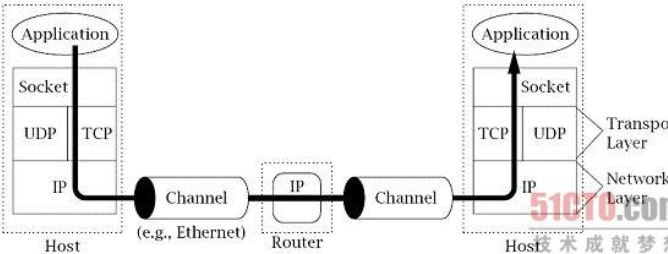
\includegraphics[scale=.6]{img/01.01.png}
			\caption{一个TCP/IP网络}
			\label{fig:tcpip.net.trans}
		\end{figure}

		Application:应用程序; Socket:套接字; Host:主机;Channel:通信信道; Ethernet:以太网; Router:路由器;Network Layer:网络层; Transport Layer:传输层。

		在 TCP/IP 协议族中,底层由基础的通信信道构成,如以太网或调制解调器拨号连接。这些信道由网络层(network layer)使用,而网络层则完成将分组报文传输到它们的目的地址的工作(也就是路由器的功能)。TCP/IP 协议族中属于网络层的唯一协议是 IP 协议,它使两个主机间的一系列通信信道和路由器看起来像是一条单一的主机到主机的信道。

		IP 协议提供了一种数据报服务:每组分组报文都由网络独立处理和分发,就像信件或包裹通过邮政系统发送一样。为了实现这个功能,每个 IP 报文必须包含一个保存其目的地址(address)的字段,就像你所投递的每份包裹都写明了收件人地址。(我们随即会对地址进行更详细的说明。)尽管绝大部分递送公司会保证将包裹送达,但 IP 协议只是一个"尽力而为"(best-effort)的协议:它试图分发每一个分组报文,但在网络传输过程中,偶尔也会发生丢失报文,使报文顺序被打乱,或重复发送报文的情况。

		IP 协议层之上称为传输层(transport layer)。它提供了两种可选择的协议:TCP 协议和UDP 协议。这两种协议都建立在 IP 层所提供的服务基础上,但根据应用程序协议(application protocols)的不同需求,它们使用了不同的方法来实现不同方式的传输。TCP 协议和 UDP协议有一个共同的功能,即寻址。回顾一下,IP 协议只是将分组报文分发到了不同的主机,很明显,还需要更细粒度的寻址将报文发送到主机中指定的应用程序,因为同一主机上可能有多个应用程序在使用网络。TCP 协议和 UDP 协议使用的地址叫做端口号(port numbers),都是用来区分同一主机中的不同应用程序。TCP 协议和 UDP 协议也称为端到端传输协议 (end-to-end transport protocols),因为它们将数据从一个应用程序传输到另一个应用程序,而 IP 协议只是将数据从一个主机传输到另一主机。

		TCP 协议能够检测和恢复 IP 层提供的主机到主机的信道中可能发生的报文丢失、重复及其他错误。TCP 协议提供了一个可信赖的字节流(reliable byte-stream)信道,这样应用程序就不需要再处理上述的问题。TCP 协议是一种面向连接(connection-oriented)的协议:在使用它进行通信之前,两个应用程序之间首先要建立一个 TCP 连接,这涉及到相互通信的两台电脑的 TCP 部件间完成的握手消息(handshake messages)的交换。使用 TCP 协议在很多方面都与文件的输入输出(I/O, Input/Output)相似。实际上,由一个程序写入的文件再由另一个程序读取就是一个 TCP 连接的适当模型。另一方面,UDP 协议并不尝试对 IP 层产生的错误进行修复,它仅仅简单地扩展了 IP 协议"尽力而为"的数据报服务,使它能够在应用程序之间工作,而不是在主机之间工作。因此,使用了 UDP 协议的应用程序必须为处理报文丢失、顺序混乱等问题做好准备。


	\section{关于地址}

		寄信的时候,要在表格中填上邮政服务能够理解的收信人的地址。在给别人打电话之前,必须给电话系统提供你所联系的人的电话号码。同样,一个程序要与另一个程序通信,就要给网络提供足够的信息,使其能够找到另一个程序。在 TCP/IP 协议中,有两部分信息用来定位一个指定的程序:互联网地址(Internet address)和端口号(port number)。其中互联网地址由 IP 协议使用,而附加的端口地址信息由传输协议(TCP 或 IP 协议)对其进行解析。

		互联网地址由二进制的数字组成,有两种型式,分别对应了两个版本的标准互联网协议。现在最常用的版本是版本 4, IPv4,即另一个版本是刚开始开发的版本 6, IPv6。即 IPv4 的地址长 32 位,只能区分大约 40 亿个独立地址,对于如今的互联网来说,这是不够大的。(也许看起来很多,但由于地址的分配方式的原因,有很多都被浪费了)出于这个原因引入了 IPv6,它的地址有 128 位长。

		为了便于人们使用互联网地址(相对于程序内部的表示),两个版本的 IP 协议有不同的表示方法。IPv4 地址被表示为一组 4 个十进制数,每两个数字之间由圆点隔开(如:10.1.2.3),这种表示方法叫做点分形式(dotted-quad)。点分形式字符串中的 4 个数字代表了互联网地址的 4 个字节,也就是说,每个数字的范围是 0 到 255。

		另一方面,IPv6 地址的 16 个字节由几组 16 进制的数字表示,这些 16 进制数之间由分号隔开(如:2000:fdb8:0000:0000:0001:00ab:853c:39a1)。每组数字分别代表了地址中的两个字节,并且每组开头的 0 可以省略,因此前面的例子中,第 5 组和第 6 组数字可以缩写为:1:ab:。甚至,只包含 0 的连续组可以全部省略(但在一个地址中只能这样做一次)。因此,前面的例子的完整地址可以表示为 2000:fdb8::1:00ab:853c:39a1。

		从技术角度来讲,每个互联网地址代表了一台主机与底层的通信信道的连接,换句话说,也就是一个网络接口(network interface)。主机可以有多个接口,这并不少见,例如一台主机同时连接了有线以太网(Ethernet)和无线网(WiFi)。由于每个这样的连接都属于唯一的一台主机,所以只要它连接到网络,一个互联网地址就能定位这条主机。但是反过来,一台主机并不对应一个互联网地址。因为每台主机可以有多个接口,每个接口又可以有多个地址。(实际上一个接口可以同时拥有 IPv4 地址和 IPv6 地址)。

		TCP 或 UDP 协议中的端口号总与一个互联网地址相关联。回到前面我们作类比的例子,一个端口号就相当于指定街道上一栋大楼的某个房间号。邮政服务通过街道地址把信分发到一个邮箱,再由清空邮箱的人把这封信递送到这栋楼的正确房间中。或者考虑一个公司的内部电话系统:要与这个公司中的某个人通话,首先要拨打该公司的总机电话号码连接到其内部电话系统,然后再拨打你要找的那个人的分机号码。在上面的例子中,互联网地址就相对于街道地址或公司的总机电话号码,端口号就相当于房间号或分机号码。端口号是一组 16位的无符号二进制数,每个端口号的范围是 1 到 65535。(0 被保留)。

		每个版本的 IP 协议都定义了一些特殊用途的地址。其中值得注意的一个是回环地址(loopback address),该地址总是被分配个一个特殊的回环接口(loopback interface)。回环接口是一种虚拟设备,它的功能只是简单地将发送给它的报文直接回发给发送者。回环接口在测试中非常有用,因为发送给这个地址的报文能够立即返回到目标地址。而且每台主机上都有回环接口,即使当这台计算机没有其他接口(也就是说没有连接到网络),回环接口也能使用。IPv4 的回环地址是 127.0.0.1[ ],IPv6 的回环地址是 0:0:0:0:0:0:0:1。

		IPv4 地址中的另一种特殊用途的保留地址包括那些"私有用途"的地址。它们包括 IPv4 中所有以 10 或 192.168 开头的地址,以及第一个数是 172,第二个数在 16 到 31 的地址。(在IPv6 中没有相应的这类地址)这类地址最初是为了在私有网络中使用而设计的,不属于公共互联网的一部分。现在这类地址通常被用在家庭或小型办公室中,这些地方通过 NAT(Network Address Translation,网络地址转换)设备连接到互联网。NAT 设备的功能就像一个路由器,转发分组报文时将转换(重写)报文中的地址和端口。更准确地说,它将一个接口中报文的私有地址端口对(private address, port pairs)映射成另一个接口中的公有地址端口对(public address, port pairs)。这就使一小组主机(如家庭网络)能够有效地共享同一个 IP 地址。重要的是这些内部地址不能从公共互联网访问。如果你在拥有私有类型地址的计算机上试验本书的例子,并试图与另一台没有这类地址的主机进行通信,通常只有这台拥有私有类型地址的主机发起的通信才能成功。

		相关的类型的地址包括本地链接(link-local),或称为"自动配置"地址。IPv4 中,这类地址由 169.254 开头,在 IPv6 中,前 16 位由 FE8 开头的地址是本地链接地址。这类地址只能用来在连接到同一网络的主机之间进行通信,路由器不会转发这类地址的信息。最后,另一类地址由多播(multicast)地址组成。普通的 IP 地址(有时也称为"单播"地址)只与唯一一个目的地址相关联,而多播地址可能与任意数量的目的地址关联。我们将在第 4 章中简要地对多播技术作进一步介绍。IPv4 中的多播地址在点分格式中,第一个数字在 224 到 239 之间。IPv6 中,多播地址由 FF 开始。 

	\section{关于名字}

		也许你更习惯于通过名字来指代一个主机,例如:host.example.com。然而,互联网协议只能处理二进制的网络地址,而不是主机名。首先应该明确的是,使用主机名而不使用地址是出于方便性的考虑,这与TCP/IP提供的基本服务是相互独立的。你也可以不使用名字来编写和使用TCP/IP应用程序。当使用名字来定位一个通信终端时,系统将做一些额外的工作把名字解析成地址。有两个原因证明这额外的步骤是值得的:

		第一,相对于点分形式(或IPv6中的十六进制数字串),人们更容易记住名字;

		第二,名字提供了一个间接层,使IP地址的变化对用户不可见。在本书第一版的写作期间,网络服务器www.mkp.com的地址就改变过。

		由于我们通常都使用网络服务器的名字,而且地址的改变很快就被反应到映射主机名和网络地址的服务上(我们马上会对其进行更多的介绍),如www.mkp.com从之前的地址208.164.121.48 对应到了现在的地址,这种变化对通过名字访问该网络服务器的程序是透明的。

		名字解析服务可以从各种各样的信息源获取信息。两个主要的信息源是域名系统(DNS,Domain Name System)和本地配置数据库。DNS[ ]是一种分布式数据库,它将像www.mkp.com这样的域名映射到真实的互联网地址和其他信息上。DNS协议允许连接到互联网的主机通过TCP或UDP协议从DNS数据库中获取信息。本地配置数据库通常是一种与具体操作系统相关的机制,用来实现本地名称与互联网地址的映射。

	\section{客户端和服务器}
		在前面的邮政和电话系统例子中,每次通信都是由发信方或打电话者发起,而另一方则通过发回反馈信或接听电话来对通信的发起者作出响应。互联网通信也与这个过程类似。客户端(client)和服务器(server)这两个术语代表了两种角色:客户端是通信的发起者,而服务器程序则被动等待客户端发起通信,并对其作出响应。客户端与服务器组成了应用程序(application)。客户端和服务器这两个术语对典型的情况作出了描述,服务器具有一定的特殊能力,如提供数据库服务,并使任何客户端能够与之通信。

		一个程序是作为客户端还是服务器,决定了它在与其对等端(peer)建立通信时使用的套接字 API 的形式(客户端的对等端是服务器,反之亦然)。更进一步来说,客户端与服务器端的区别非常重要,因为客户端首先需要知道服务器的地址和端口号,反之则不需要。如果有必要,服务器可以使用套接字 API,从收到的第一个客户端通信消息中获取其地址信息。这与打电话非常相似:被呼叫者不需要知道拨电话者的电话号码。就像打电话一样,只要通信连接建立成功,服务器和客户端之间就没有区别了。

		客户端如何才能找到服务器的地址和端口号呢?通常情况,客户端知道服务器的名字,例如使用URL(Universal Resource Locator,统一资源定位符)如http://www.mkp.com,再通过名字解析服务获取其相应的互联网地址。

		获取服务器的端口号则是另一种情况。从原理上来讲,服务器可以使用任何端口号,但客户端必须能够获知这些端口号。在互联网上,一些常用的端口号被约定赋给了某些应用程序。例如,端口号 21 被FTP(File Transfer Protocol,文件传输协议)使用。当你运行FTP客户端应用程序时,它将默认通过这个端口号连接服务器。互联网的端口号授权机构维护了一个包含所有已约定使用的端口号列表(见http://www.iana.org/assignments/port-numbers)。

	\section{什么是套接字}

		Socket(套接字)是一种抽象层,应用程序通过它来发送和接收数据,就像应用程序打开一个文件句柄,将数据读写到稳定的存储器上一样。一个 socket 允许应用程序添加到网络中,并与处于同一个网络中的其他应用程序进行通信。一台计算机上的应用程序向 socket写入的信息能够被另一台计算机上的另一个应用程序读取,反之亦然。

		不同类型的 socket 与不同类型的底层协议族以及同一协议族中的不同协议栈相关联,本书只涵盖了 TCP/IP 协议族的内容。现在 TCP/IP 协议族中的主要 socket 类型为流套接字(sockets sockets)和数据报套接字(datagram sockets)。流套接字将 TCP 作为其端对端协议(底层使用 IP 协议),提供了一个可信赖的字节流服务。一个 TCP/IP 流套接字代表了 TCP 连接的一端。数据报套接字使用 UDP 协议(底层同样使用 IP 协议),提供了一个"尽力而为"(best-effort)的数据报服务,应用程序可以通过它发送最长 65500 字节的个人信息。当然,其他协议族也支持流套接字和数据报套接字,但本书只对 TCP 流套接字和 UDP 数据报套接字进行讨论。一个 TCP/IP 套接字由一个互联网地址,一个端对端协议(TCP 或 UDP 协议)以及一个端口号唯一确定。随着进一步学习,你将了解到把一个套接字绑定到一个互联网地址上的多种方法。

		图 1.2 描述了一个主机中,应用程序、套接字抽象层、协议、端口号之间的逻辑关系。
		\begin{figure}[htbp]%位置选项
			\centering
			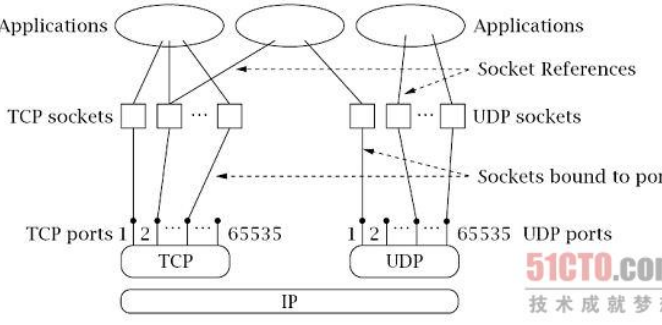
\includegraphics[scale=.6]{img/01.02.png}
			\caption{套接字、协议、端口}
			\label{fig:socket.trans}
		\end{figure}

		Applications:应用程序;TCP sockets:TCP 套接字;TCP ports:TCP 端口;Socket References:套接字引用;UDP sockets:UDP 套接字;Sockets bound to ports:套接字绑定到 端口;UDP ports:UDP 端口。

		值得注意的是一个套接字抽象层可以被多个应用程序引用。每个使用了特定套接字的程序都可以通过那个套接字进行通信。前面已提到,每个端口都标识了一台主机上的一个应用程序。实际上,一个端口确定了一台主机上的一个套接字。从图 1.2 中我们可以看到,主机中的多个程序可以同时访问同一个套接字。在实际应用中,访问相同套接字的不同程序通常都属于同一个应用(例如,Web 服务程序的多个拷贝),但从理论上讲,它们是可以属于不同应用的。




	\part{Java API}

		
\chapter{基本套接字}

	\section{套接字地址}

		\subsection{例子}

		\lstinputlisting[]{src/ch02/InetAddressExample.java}

		运行与输出结果:

\begin{lstlisting}[language=Bash]
% java InetAddressExample \
	www.baidu.com www.jadehahaha.com \
	129.35.69.7

Interface eth0:
	Address (v6): fe80:0:0:0:225:b3ff:fe69:1659%2
	Address (v4): 172.16.7.1
Interface lo:
	Address (v6): 0:0:0:0:0:0:0:1%1
	Address (v4): 127.0.0.1
www.baidu.com: 
	www.baidu.com/220.181.111.147
www.jadehahaha.com: 
	Unable to find address for : www.jadehahaha.com
129.35.69.7: 
	129.35.69.7/129.35.69.7
\end{lstlisting}

		\subsection{InetAddress类API简介}

			InetAddress类中创建与访问实例方法:
\begin{lstlisting}
static InetAddress [] getAllByName(String host);
static InetAddress getByName(String host);
static InetAddress getLocalHost();
/**
 * return byte array as ip address
 * size if 4 byte in ipv4
 * or size is 16 in ipv6
 */
byte[] getAddress();
\end{lstlisting}

			InetAddress类中字符串显示方法:
\begin{lstlisting}
/**
 * return value format like:
 *   hostname.example.com/192.0.2.127
 *   or
 *   never.example.net/2000::620:1a30:95b2
 */
String toString();
String getHostAddress();
/**
 * return host name
 */
String getHostName();
/**
 * return host name ()
 */
String getCanonicalHostName();
\end{lstlisting}

			InetAddress类中检查属性的方法:
\begin{lstlisting}
boolean isAnyLocalAddress();
boolean isLinkLocalAddress();
boolean isLoopBackAddress();
// 是否为多播地址
boolean isMulticastAddress();
// 测试多播地址范围:global
boolean isMCGlobal();
// 测试多播地址范围:link local
boolean isMCLinkLocal();
// 测试多播地址范围:node local
boolean isMCNodeLocal();
// 测试多播地址范围:org local
boolean isMCOrgLocal();
// 测试多播地址范围:site local
boolean isMCSiteLocal();
boolean isReachable(int timeout);
boolean isReachable(NetworkInterface netif, int ttl, int timeout)
\end{lstlisting}


	\section{TCP套接字}

		\chapter{发送和接收数据}

通常情况下,在程序中使用套接字是因为需要向其他程序提供信息,或使用其他程序提供的信息。这并不是什么魔法:任何要交换信息的程序之间在信息的编码方式上必须达成共识(如将信息表示为位序列),以及哪个程序发送信息,什么时候和怎样接收信息都将影响程序的行为。程序间达成的这种包含了信息交换的形式和意义的共识称为协议,用来实现特定应用程序的协议叫做应用程序协议。前面章节中的回馈程序示例中的应用程序协议都过于简单:客户端和服务器的行为都不受它们之间所交换的信息内容的影响。而在绝大部分实际应用中,客户端和服务器的行为都要依赖于它们所交换的信息,因此应用程序协议通常更加复杂。 

TCP/IP协议以字节的方式传输用户数据,并没有对其进行检查和修改。这个特点使应用程序可以非常灵活地对其传输的信息进行编码。大部分的应用程序协议是根据由字段序列组成的离散信息定义的,其中每个字段中都包含了一段以位序列编码的特定的信息。应用程序协议中明确定义了信息的发送者应该怎样排列和解释这些位序列,同时还要定义接收者应该怎样解析,这样才使信息的接收者能够抽取出每个字段的意义。TCP/IP协议的唯一约束是,信息必须在块(chunks)中发送和接收,而块的长度必须是8位的倍数,因此,我们可以认为在TCP/IP协议中传输的信息是字节序列。鉴于此,我们可以进一步把传输的信息看作数字序列或数组,每个数字的取值范围是0到255。这与8位编码的二进制数值范围是一致的:00000000代表0,00000001代表1,00000010代表2,等等,最多到11111111,即255。 

如果你建立了一个程序使用套接字与其他程序交换信息,通常符合下面两种情况之一:

要么是你设计和编写了套接字的客户端和服务器端,这种情况下你能够随心所欲地定义自己的应用程序协议;

要么是你实现了一个已经存在的协议,或许是一个协议标准。

任何一种情况,在"线路上"将不同类型的信息进行字节编码和解码的基本原理还是一样的。顺便说一下,如果"线路"是由一个程序写,由另一程序读的文件,本章的所有内容对其也是适用的。 

\section{信息编码} 

	首先,我们来考虑一下简单数据类型,如int,long,char,String等,是如何通过套接字发送和接收的。从前面章节我们已经知道,传输信息时可以通过套接字将字节信息写入一个OutputStream实例中(该实例已经与一个Socket相关联),或将其封装进一个DatagramPacket实例中(该实例将由DatagramSocket发送)。然而,这些操作所能处理的唯一数据类型是字节和字节数组。作为一种强类型语言,Java需要把其他数据类型(int,String等)显式转换成字节数组。所幸的是Java的内置工具能够帮助我们完成这些转换。在第2.2.1节的TCPEchoClient.java示例程序中,我们看到过String类的getBytes()方法,该方法就是将一个Sring实例中的字符转换成字节的标准方式。在考虑数据类型转换的细节之前,我们先来看看大部分基本数据类型的表示方法。 

	\subsection{基本整型} 

		如我们所见,TCP和UDP套接字使我们能发送和接收字节序列(数组),即范围在0-255之间的整数。使用这个功能,我们可以对值更大的基本整型数据进行编码,不过发送者和接收者必须先在一些方面达成共识。一是要传输的每个整数的字节大小(size)。例如,Java程序中,int数据类型由32位表示,因此,我们可以使用4个字节来传输任意的int型变量或常量;short数据类型由16位表示,传输short类型的数据只需要两个字节;同理,传输64位的long类型数据则需要8个字节。 

		下面我们考虑如何对一个包含了4个整数的序列进行编码:一个byte型,一个short型,一个int型,以及一个long型,按照这个顺序从发送者传输到接收者。我们总共需要15个字节:第一个字节存放byte型数据,接下来两个字节存放short型数据,再后面4个字节存放int型数据,最后8个字节存放long型数据,如下所示: 

		\lstinputlisting[language=Java,firstline=1,lastline=2]{src/ch03/BruteForceCoding.txt}

		我们已经做好深入研究的准备了吗?未必。对于需要超过一个字节来表示的数据类型,我们必须知道这些字节的发送顺序。显然有两种选择:从整数的右边开始,由低位到高位地发送,即little-endian顺序;或从左边开始,由高位到低位发送,即big-endian顺序。(注意,幸运的是字节中位的顺序在实现时是以标准的方式处理的)考虑长整型数123456787654321L,其64位(以十六进制形式)表示为0x0000704885F926B1。
		
		如果我们以big-endian顺序来传输这个整数,其字节的十进制数值序列就如下所示: 

		\lstinputlisting[language=Java,firstline=12,lastline=15]{src/ch03/BruteForceCoding.txt}

		如果我们以little-endian顺序传输,则字节的十进制数组序列为: 

		\lstinputlisting[language=Java,firstline=17,lastline=20]{src/ch03/BruteForceCoding.txt}

		关键的一点是,对于任何多字节的整数,发送者和接收者必须在使用big-endian顺序还是使用little-endian顺序上达成共识。如果发送者使用了little-endian顺序来发送上述整数,而接收者以big-endian顺序对其进行接收,那么接收者将取到错误的值,它会将这个8字节序列的整数解析成12765164544669515776L。 

		Java中的ByteOrder类中有两个常量: \verb|BIG_ENDIAN| 和 \verb|LITTLE_ENDIAN| 来表示大端与小端。

		发送者和接收者需要达成共识的最后一个细节是:所传输的数值是有符号的(signed)还是无符号的(unsigned)。Java中的四种基本整型都是有符号的,它们的值以二进制补码(two's-complement)的方式存储,这是有符号数值的常用表示方式。在处理有k位的有符号数时,用二进制补码的形式表示负整数-n(1 ≤ n ≤ $2^{k-1}$),则补码的二进制值就为$2^k-n$。而对于非负整数p(0 ≤ p ≤ $2^{k-1}-1$),只是简单地用k位二进制数来表示p的值。因此,对于给定的k位,我们可以通过二进制补码来表示$-2^{k-1}$到$2^{k-1}-1$范围的值。注意,最高位(msb)标识了该数是正数(msb = 0)还是负数(msb = 1)。另外,如果使用无符号(unsigned)编码,k位可以直接表示0到$2^k-1$之间的数值。例如,32位数值0xffffffff(所有位全为1),将其解析为有符号数时,二进制补码整数表示-1;将其解析为无符号数时,它表示4294967295。由于Java并不支持无符号整型,如果要在Java中编码和解码无符号数,则需要做一点额外的工作。在此假设我们处理的都是有符号整数数据。 

		那么我们怎样才能将消息的正确值存入字节数组呢?为了清楚地展示需要做的步骤,我们将对如何使用"位操作(bit-diddling)"(移位和屏蔽)来显式编码进行介绍。示例程序BruteForceCoding.java中有一个特殊的方法encodeIntBigEndian()能够对任何值的基本类型数据进行编码。它的参数包括用来存放数值的字节数组,要进行编码的数值(表示为long型,它是最长的整型,能够保存其他整型的值),数值在字节数组中开始位置的偏移量,以及该数值写到数组中的字节数。如果我们在发送端进行了编码,那么必须能够在接收端进行解码。BruteForceCoding类同时还提供了decodeIntBigEndian()方法,用来将字节数组的子集解码到一个Java的long型整数中。 

		\lstinputlisting[language=Java,firstline=1]{src/ch03/BruteForceCoding.java}

		1. 数据项编码:第5-8行 

		2. Java中的基本整数所占字节数:第10-13行 

		3. byteArrayToDecimalString():第17-23行 

		该方法把给定数组中的每个字节作为一个无符号十进制数打印出来。BYTEMASK的作用是防止在字节数值转换成int类型时,发生符号扩展(sign-extended),即转换成无符号整型。 

		4.encodeIntBigEndian():第26-32行 

		赋值语句的右边,首先将数值向右移动,以使我们需要的字节处于该数值的低8位中。然后,将移位后的数转换成byte型,并存入字节数组的适当位置。在转换过程中,除了低8位以外,其他位都将丢弃。这个过程将根据给定数值所占字节数迭代进行。该方法还将返回存入数值后字节数组中新的偏移位置,因此我们不必做额外的工作来跟踪偏移量。 

		5. decodeIntBigEndian():第35-42行 

		根据给定数组的字节大小进行迭代,通过每次迭代的左移操作,将所取得字节的值累积到一个long型整数中。 

		6. 示例方法:第44-67行 

		准备接收整数序列的数组:第45行 

		对每项进行编码:第47-50行 

		对byte,short,int以及long型整数进行编码,并按照前面描述的顺序存入字节数组。 

		打印编码后数组的内容:第51行 

		对编码字节数组中的某些字段进行解码:第55-57行 

		解码后输出的值应该与编码前的原始值相等。 

		转换问题:第61-66行 

		在字节数组偏移量为4的位置,该字节的十进制值是245,然而,当将其作为一个有符号字节读取时,其值则为-11(回忆有符号整数的二进制补码表示方法)。如果我们将返回值直接存入一个long型整数,它只是简单地变成这个long型整数的最后一个字节,值为245。如果将返回值放入一个字节型整数,其值则为-11。到底哪个值正确取决于你的应用程序。如果你从N个字节解码后希望得到一个有符号的数值,就必须将解码结果(长的结果)存入一个刚好占用N个字节的基本整型中。如果你希望得到一个无符号的数组,就必须将解码结果存入更长的基本整型中,该整型至少要占用N+1个字节。 

		注意,在encodeIntBigEndian() 和 decodeIntBigEndian()方法的开始部分,我们可能需要做一些前提条件检测,如0 ≤ size ≤ 8 和 dst ≠ null等。你能举出需要做的其他前期检测吗? 

		运行以上程序,其输出显示了一下字节的值(以十进制形式): 

		\lstinputlisting[language=Java,firstline=31,lastline=34]{src/ch03/BruteForceCoding.txt}

		如你所见,上面的强制(brute-force)编码方法需要程序员做很多工作:要计算和命名每个数值的偏移量和大小,并要为编码过程提供合适的参数。如果没有将encodeIntBigEndian()方法提出来作为一个独立的方法,情况会更糟。基于以上原因,强制编码方法是不推荐使用的,而且Java也提供了一些更加易用的内置机制。不过,值得注意的是强制编码方法也有它的优势,除了能够对标准的Java整型进行编码外,encodeIntegerBigEndian() 方法对1到8字节的任何整数都适用--例如,如果愿意的话,你可以对一个7字节的整数进行编码。 

		构建本例中的消息的一个相对简单的方法是使用DataOutputStream类和ByteArrayOutputStream类。DataOutputStream 类允许你将基本数据类型,如上述整型,写入一个流中:它提供了writeByte(),writeShort(),writeInt(),以及writeLong()方法,这些方 按照big-endian顺序,将整数以适当大小的二进制补码的形式写到流中。ByteArrayOutputStream类获取写到流中的字节序列,并将其转换成一个字节数组。用这两个类来构建我们的消息的代码如下: 

		\lstinputlisting[language=Java,firstline=41,lastline=48]{src/ch03/BruteForceCoding.txt}

		也许你想运行这段代码,来证实它与BruteForceEncoding.java的输出结果一样。 

		讲了这么多发送方相关的内容,那么接收方将如何恢复传输的数据呢?正如你想的那样,Java中也提供了与输出工具类相似的输入工具类,分别是DataInputStream类和ByteArrayInputStream类。在后面讨论如何解析传入的消息时,我们将对这两个类的使用举例。并且,在第5章中,我们还会看到另一种方法,使用ByteBuffer类将基本数据类型转换成字节序列。 

		最后,本节的所有内容基本上也适用于BigInteger类,该类支持任意大的整数。对于基本整型,发送者和接收者必须在使用多大空间(字节数)来表示一个数值上达成共识。但是这又与使用BigInteger相矛盾,因为BigInteger可以是任意大小。一种解决方法是使用基于长度的帧,我们将在第3.3节看到这种方法。 


	\subsection{字符串和文本} 

		历史悠久的文本(可打印,即可显示的字符串)可能是用来表示信息最常用的方式。文本使用起来非常方便,因为人们习惯于处理各种各样以字符串形式表示的信息,如书本中,报纸中,以及电脑显示器上的信息。因此,只要我们指定如何对要传输的文本进行编码,我们就几乎能发送其他任何类型的数据:先将其表示成文本形式,再对文本进行编码。显然,我们可以将数字和boolean类型的数据表示成String类型,如"123478962","6.02e23","true","false"等。我们也已经看到,通过调用getBytes()方法,可以将一个字符串转换成字节数组(见TCPEchoClient.java)。当然,还有其他方法实现这个功能。 

		为了更好地理解这个过程,我们首先得将文本视为由符号和字符(characters)组成。实际上每个String实例都对应了一个字符序列(数组,char[]类型)。一个字符在Java内部表示为一个整数。例如,字符"a",即字母"a"的符号,与整数97对应;字符"X"对应了88,而符号"!"(感叹号)则对应了33。 

		在一组符号与一组整数之间的映射称为编码字符集(coded character set.)。或许你听说过ASCII编码字符集(ASCII,American Standard Code for Information Interchange,美国标准信息交换码)。ASCII码将英语字母、数字、标点符号以及一些特殊符号(不可打印字符)映射成0到127的整数。自20世纪60年代以来,ASCII码就被用来进行数据传输,甚至在今天,它也广泛应用在应用程序协议中,如HTTP(万维网所用的协议)。然而,由于它忽略了许多英语以外的其他语言所使用的符号,在如今全球化经济环境下,使用ASCII码来开发应用程序和设计协议就显得不够理想。 

		因此,Java使用了一种称为Unicode的国际标准编码字符集来表示char型和String型值。Unicode字符集将"世界上大部分的语言和符号"[ ]映射到整数0至65535之间,能更好地适用于国际化程序。例如,日文平假名中代表音节"o"的符号映射成了整数12362。Unicode包含了ASCII码:每个ASCII码中定义的符号在Unicode中所映射整数与其在ASCII码中映射的整数相同。这就为ASCII与Unicode之间提供了一定程度的向后兼容性。 

		发送者与接收者必须在符号与整数的映射方式上达成共识,才能使用文本信息进行通信。这就是他们所要达成一致的所有内容吗?还得根据情况而定。对于每个整数值都比255小的一小组字符,则不需要其他信息,因为其每个字符都能够作为一个单独的字节进行编码。对于可能使用超过一个字节的大整数的编码方式,就有多种方式在线路上对其进行编码。因此,发送者和接收者还需要对这些整数如何表示成字节序列统一意见,即编码方案(encoding cheme)。编码字符集和字符的编码方案结合起来称为字符集(charset,见RFC 2278)。你也可以定义自己的字符集,但没有理由这样做,世界上已经有大量不同的标准(standardized)字符集在使用。Java提供了对任意字符集的支持,而且每种实现都必须支持以下至少一种字符集:US-ASCII(ASCII的另一个名字),ISO-8859-1,UTF-8,UTF-16BE,UTF-16LE,UTF-16。 

		调用String实例的getBytes()方法,将返回一个字节数组,该数组根据平台默认字符集(default charset)对String实例进行了编码。很多平台的默认字符集都是UTF-8,然而在一些经常使用ASCII字符集以外的字符的地区,情况有所不同。要保证一个字符串按照特定(particular)字符集编码,只需要将该字符集的名字作为参数(String类型)传递给getBytes()方法,其返回的字节数组就包含了由指定字符集表示的字符串。(注意,在第2.2.1节的TCP回显客户端/服务器示例程序与编码是无关的,因为它们根本没有对接收到的数据进行解释。) 

		下面举例来对getBytes()方法进行说明。如果在著作本书的平台上调用
		
		\verb|"Test!".getBytes()|,你将获得按照UTF-8字符集编码的字节数组;

		\lstinputlisting[language=Java,firstline=51,lastline=53]{src/ch03/BruteForceCoding.txt}

		然而如果你调用\verb|"Test!".getBytes("UTF-16BE")|你将得到如下数组:在这种情况下每个值被编码成了两个字节的序列,高位在前; 
		
		\lstinputlisting[language=Java,firstline=55,lastline=57]{src/ch03/BruteForceCoding.txt}

		如果调用 "Test!".getBytes("IBM037"),返回结果将是: 

		\lstinputlisting[language=Java,firstline=59,lastline=61]{src/ch03/BruteForceCoding.txt}

		上面的例子说明,发送者和接收者必须在文本字符串的表示方式上达成共识。最简单的方法就是定义一个标准字符集。 

		我们知道,可以通过先将字符串转换成独立的字节,再将其写到流中的方式,把String写入到OutputStream中去。这个方法在每次调用getBytes()方法时,都得指定编码方式。在本章后续内容中,我们将看到只需要简单指定一次编码就能构建文本消息的方法。 

	\subsection{位操作:布尔值编码}

		位图(Bitmaps)是对布尔信息进行编码的一种非常紧凑的方式,通常用在协议中。位图的主要思想是整型数据中的每一位都能够对一个布尔值编码--通常是0表示false,1表示true。要操纵位图,你需要了解如何使用Java中的"位操作"方法来设置和清除单独的一位。掩码(mask)是一个的整数值,其中有一位或多位被设为1,其他各位被清空(即,设为0)。在这里我们处理的是int大小的位图和掩码(32位),但这些方法对其他类型的整数也同样适用。 

		我们将int中的各位从0到31进行编号,其中0代表最低位。一般来说,如果一个int值在第i位值为1,其他位都为0的话,该int型整数的值就是$2^i$。因此编号为5的位表示32,编号为12的位表示4096,等等。这里有一些掩码声明的例子: 

		\lstinputlisting[language=Java,firstline=71,lastline=74]{src/ch03/BruteForceCoding.txt}


		要设置int变量中的特定一位,需要将该int值与特定位对应的掩码进行按位或(bitwise-OR)操作(|): 

		\lstinputlisting[language=Java,firstline=76,lastline=76]{src/ch03/BruteForceCoding.txt}

		要清空特定一位,则将该整数与特定所对应的掩码的按位补码(特定位为0,其他位为1)进行按位与(bitwise-AND)操作。Java中的按位与操作符是\verb|&|,而按位补码操作符是\verb|~|: 

		\lstinputlisting[language=Java,firstline=78,lastline=78]{src/ch03/BruteForceCoding.txt}

		也可以通过将相应的所有掩码进行按位或操作,一次设置和清空多位: 

		\lstinputlisting[language=Java,firstline=80,lastline=81]{src/ch03/BruteForceCoding.txt}

		要测试一个整数的特定位是否已经被设置,可以将该整数与特定位对应的掩码进行按位与,并将操作结果与0比较: 

		\lstinputlisting[language=Java,firstline=83,lastline=83]{src/ch03/BruteForceCoding.txt}


\section{组合输入输出流}

	Java中与流相关的类可以组合起来从而提供强大的功能。例如,我们可以将一个Socket实例的OutputStream包装在一个BufferedOutputStream实例中,这样可以先将字节暂时缓存在一起,然后再一次全部发送到底层的通信信道中,以提高程序的性能。我们还能再将这个BufferedOutputStream实例包裹在一个DataOutputStream实例中,以实现发送基本数据类型的功能。以下是实现这种组合的代码: 

	\lstinputlisting[language=Java,firstline=91,lastline=93]{src/ch03/BruteForceCoding.txt}

	\begin{figure}[htbp]%位置选项
		\centering
		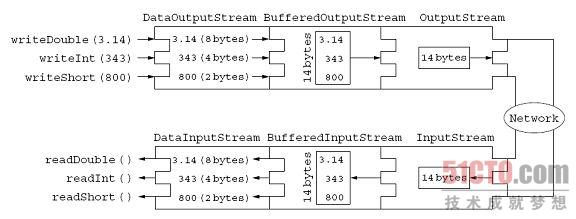
\includegraphics[scale=.8]{img/03.01.jpg}
		\caption{流组合}
		\label{fig:comp.stream}
	\end{figure}

	图3.1展示了这中组合。在这个例子中,我们先将基本数据的值,一个一个写入DataOutputStream中,DataOutputStream再将这些数据以二进制的形式写入BufferedOutputStream将三次写入的数据缓存起来,然后再由BufferedOutputStream一次性地将这些数据写入套接字的OutputStream,最后由OutputStream将数据发送到网络。在另一个终端,我们创建了相应的组合InputStream,以有效地接收基本数据类型。 

	对Java输入输出API的完整介绍不在本书的讨论范围中,不过,表3.1列出了一些相关的Java输入输出类,为介绍它们的强大功能起一个抛砖引玉的作用。Java基本输入输出类:

	Buffered[Input/Output]Stream 通过缓存性能优化

	Checked[Input/Output]Stream  维护数据检查

	Cipher[Input/Output]Stream   加密/解密 

	Data[Input/Output]Stream     数据处理 

	Digest[Input/Output]Stream   维护数据摘要 

	GZIP[Input/Output]Stream     压缩/解压缩 

	Object[Input/Output]Stream   数据处理 

	PushbackInputStream          允许一个字节或是字节是“末读的”

	PrintOutputStream            输出数据类型的字符串表示法

	Zip[Input/Output]Stream      以zip格式

\section{成帧与解析} 

	当然,将数据转换成在线路上传输的格式只完成了一半工作,在接收端还必须将接收到的字节序列还原成原始信息。应用程序协议通常处理的是由一组字段组成的离散的信息。成帧(Framing)技术则解决了接收端如何定位消息的首尾位置的问题。无论信息是编码成了文本、多字节二进制数、或是两者的结合,应用程序协议必须指定消息的接收者如何确定何时消息已完整接收。 

	如果一条完整的消息负载在一个DatagramPacket中发送,这个问题就变得很简单了:DatagramPacket 负载的数据有一个确定的长度,接收者能够准确地知道消息的结束位置。然而,如果通过TCP套接字来发送消息,情况将变得更复杂,因为TCP协议中没有消息边界的概念。如果一个消息中的所有字段都有固定的长度,同时每个消息又是由固定数量的字段组成的话,消息的长度就能够确定,接收者就可以简单地将消息长度对应的字节数读到一个byte[]缓存区中。在TCPEchoClient.java示例程序中我们就是用的这个方法,在该例中我们能从服务器获得消息的字节数。但是如果消息的长度是可变的(例如消息中包含了一些变长的文本字符串),我们事先就无法知道需要读取多少字节。 

	如果接收者试图从套接字中读取比消息本身更多的字节,将可能发生以下两种情况之一:如果信道中没有其他消息,接收者将阻塞等待,同时无法处理接收到的消息;如果发送者也在等待接收端的响应信息,则会形成死锁(deadlock);另一方面,如果信道中还有其他消息,则接收者会将后面消息的一部分甚至全部读到第一条消息中去,这将产生一些协议错误。因此,在使用TCP套接字时,成帧就是一个非常重要的考虑因素。 

	一些相同的考虑也适用于查找消息中每个字段的边界:接收者需要知道每个字段的结束位置和下一个字段的开始位置。因此,我们在此介绍的消息成帧技术几乎都可以应用到字段上。然而,最简单并使代码最简洁的方法是将这两个问题分开处理:首先定位消息的结束位置,然后将消息作为一个整体进行解析。在此我们专注于将整个消息作为一帧进行处理。

	主要有两个技术使接收者能够准确地找到消息的结束位置: 

	基于定界符(Delimiter-based):消息的结束由一个唯一的标记(unique marker,)指出,即发送者在传输完数据后显式添加的一个特殊字节序列。这个特殊标记不能在传输的数据中出现。 

	显式长度(Explicit length):在变长字段或消息前附加一个固定大小的字段,用来指示该字段或消息中包含了多少字节。 

	基于定界符的方法的一个特殊情况是,可以用在TCP连接上传输的最后一个消息上:

	在发送完这个消息后,发送者就简单地关闭(使用shutdownOutput()或close()方法)发送端的TCP连接。接收者读取完这条消息的最后一个字节后,将接收到一个流结束标记(即read()方法返回-1),该标记指示出已经读取到达了消息的末尾。 

	基于定界符的方法通常用在以文本方式编码的消息中:定义一个特殊的字符或字符串来标识消息的结束。接收者只需要简单地扫描输入信息(以字节的方式)来查找定界序列,并将定界符前面的字符串返回。这种方法的缺点是消息本身不能包含有定界字符,否则接收者将提前认为消息已经结束。在基于定界符的成帧方法中,发送者要保证满足这个先决条件。幸运的是,填充(stuffing)技术能够对消息中出现才定界符进行修改,从而是接收者不将其识别为定界符。在接收者扫描定界符时,还能识别出修改过的数据,并在输出消息中对其进行还原,从而使其与原始消息一致。这个技术的缺点是发送者和接收者双方都必须扫描消息。 

	基于长度的方法更简单一些,不过要使用这种方法必须知道消息长度的上限。发送者先要确定消息的长度,将长度信息存入一个整数,作为消息的前缀。消息的长度上限定义了用来编码消息长度所需要的字节数:如果消息的长度小于256字节,则需要1个字节;如果消息的长度小于65536字节,则需要2个字节,等等。 

	为了展示以上技术,我们将介绍下面定义的Framer接口。它有两个方法:frameMsg()方法用来添加成帧信息并将指定消息输出到指定流,nextMsg()方法则扫描指定的流,从中抽取出下一条消息。 

	\lstinputlisting[language=Java,firstline=1,lastline=12]{src/ch03/Framer.java}

	DelimFramer.java类实现了基于定界符的成帧方法,其定界符为"换行"符(\verb|"\n"|, 字节值为10)。 frameMethod()方法并没有实现填充,当成帧的字节序列中包含有定界符时,它只是简单地抛出异常。(扩展该方法以实现填充功能将作为练习留给读者)nextMsg()方法扫描流,直到读取到了定界符,并返回定界符前面的所有字符,如果流为空则返回null。如果累积了一个消息的不少字符,但直到流结束也没有找到定界符,程序将抛出一个异常来指示成帧错误。 

	\lstinputlisting[language=Java,firstline=1,lastline=50]{src/ch03/DelimFramer.java}

	1.构造函数:第14行 

	获取消息的输入流作为参数传递给该函数。 

	2.frameMsg() 方法用于添加帧信息:第18-28行 

	校验消息形式的有效性:第20-24行 

	检查消息中是否包含了定界符,如果包含,则抛出一个异常。 

	写消息:第25行 

	将成帧的消息输出到流中。 

	写定界符:第26行 

	3. nextMsg()方法从输入中提取消息:第30-48行 

	读取流中的每个字节,直到遇到定界符为止:第35行 

	处理流的终点:第36-43行 

	如果在遇到定界符之前就已经到了流的终点,则分两种情况:一是从帧的构造开始或从遇到前一个定界符以来,缓存区已经接收了一些字节,这时程序将抛出一个异常;否则nextMsg()方法将返回null以表示全部消息已接收完。 

	将无定界符的字节写入消息缓存区:第44行 

	将消息缓存区中的内容以字节数组的形式返回:第47行 

	我们的定界符帧有一个限制,即它不支持多字节定界符。如何对其进行修改以支持多字节定界符将作为练习留给我们的读者。 

	LengthFramer.java类实现了基于长度的成帧方法,适用于长度小于65535 ($2^{16}-1$)字节的消息。发送者首先给出指定消息的长度,并将长度信息以big-endian顺序存入两个字节的整数中,再将这两个字节放在完整的消息内容前,连同消息一起写入输出流。在接收端,我们使用DataInputStream以读取整型的长度信息;readFully() 方法将阻塞等待,直到给定的数组完全填满,这正是我们需要的。值得注意的是,使用这种成帧方法,发送者不需要检查要成帧的消息内容,而只需要检查消息的长度是否超出了限制。 

	\lstinputlisting[language=Java,firstline=1,lastline=57]{src/ch03/LengthFramer.java}

	1. 构造函数:

	获取帧消息源的输入流,并将其包裹在一个DataInputStream中。 

	2. frameMsg()方法用来添加成帧信息:

	校验消息长度:第22行 

	由于我们用的是长为两个字节的字段,因此消息的长度不能超过65535。(注意该值太
	大而不能存入一个short型整数中,因此我们每次只向输出流写一个字节)。 

	输出长度字段:第26-27行 

	添加长度信息(无符号short型整数)前缀,输出消息的字节数。 

	输出消息:第28行 

	3.nextMsg()方法用于从输入流中提取下一帧:第30-41行 

	读取长度前缀:第34-38行 

	readUnsignedShort()方法读取两个字节,将它们作为big-endian整数进行解释,并以int
	型整数返回它们的值。 

	读取指定数量的字节:第40-41行 

	readfully() 将阻塞等待,直到接收到足够的字节来填满指定的数组。 

	以字节的形式返回消息:第40行 


\section{Java特定编码}

	当你使用套接字时,通常要么是你需要同时创建通信信道两端的程序(这种情况下你也拥有了协议的完全控制权),要么实现一个给定的协议进行通信。如果你知道(i)通信双方都使用Java实现,而且(ii)你拥有对协议的完全控制权,那么就可以使用Java的内置工具如Serializable接口或远程方法调用(Remote Method Invocation,RMI)工具。RMI能够调用不同Java虚拟机上的方法,并隐藏了所有繁琐的参数编码解码细节。序列化(Serialization)处理了将实际的Java对象转换成字节序列的工作,因此你可以在不同虚拟机之间传递Java对象实例。

	这些能力可能就好像沟通的涅槃,但是在实际中,由于种种原因,它们并不总是最好的解决方案。首先,由于它们都是很笼统的工具,因而在通信开销上不能做到最高效。例如,一个对象的序列化形式,其包含的信息在Java虚拟机(JVM)环境以外是毫无意义的。其次,Serializable和Externalizable接口不能用于已经定义了不同传输格式的情况--如一个标准的协议。最后,用户自定义的类必须自己实现它们的序列化接口,而这项工作很容易出错。再强调一次,在某些情况下,这些Java的内置工具的确很有用,但是有些时候,"实现你自己的方法"可能更简单、容易或更有效。 


\section{构建和解析协议消息}

	本章结束时我们再看一个简单的例子,对在实现别人定义的协议时可能用到的技术进行了介绍。这个例子程序是一个简单的"投票"协议,如图3.2所示。这里,一个客户端向服务器发送了一个请求消息,消息中包含了一个候选人ID,范围是0至1000。 


	\begin{figure}[htbp]%位置选项
		\centering
		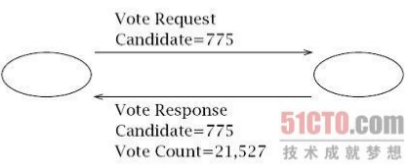
\includegraphics[scale=.8]{img/03.02.png}
		\caption{投票协议}
		\label{fig:vote.prot}
	\end{figure}

	Vote Reques:投票请求, Candidate:候选人,Vote Count:选票总数 

	程序支持两种请求。一种是查询(inquiry),即向服务器询问给定候选人当前获得的投票总数。服务器发回一个响应消息,包含了原来的候选人ID和该候选人当前(查询请求收到时)获得的选票总数。另一种是投票(voting)请求,即向指定候选人投一票。服务器对这种请求也发回响应消息,包含了候选人ID和其获得的选票数(包括了刚投的一票)。 

	在实现一个协议时,定义一个专门的类来存放消息中所包含的信息是大有裨益的。该类提供了操作消息中的字段的方法--同时用来维护不同字段之间的不变量。在我们的例子中,客户端和服务器端发送的消息都非常简单,它们唯一的区别是服务器端发送的消息包含了选票总数和一个表示响应消息(不是请求消息)的标志。因此,我们可以用一个类来表示客户端和服务器端的两种消息。VoteMsg.java类展示了每条消息中的基本信息: 

	布尔值isInquiry,其值为true时表示该消息是查询请求(为false时表示该消息是投票信息); 

	布尔值isResponse,指示该消息是响应(由服务器发送)还是请求;

	整型变量candidateID指示了候选人的ID; 

	长整型变量voteCount指示出所查询的候选人获得的总选票数。 

	这个类还维护了以下字段间的不变量: 

	candidateID的范围是0到1000。 

	voteCount在响应消息中只能是一个非零值(isResponse为true)。 

	voteCount 不能为负数。 

	\lstinputlisting[language=Java,firstline=1]{src/ch03/VoteMsg.java}

	现在我们有了一个用Java表示的投票消息,还需要根据一定的协议来对其进行编码和解码。VoteMsgCoder接口提供了对投票消息进行序列化和反序列化的方法。 

	\lstinputlisting[language=Java,firstline=1]{src/ch03/VoteMsgCoder.java}

	toWire()方法用于根据一个特定的协议,将投票消息转换成一个字节序列,fromWire()方法则根据相同的协议,对给定的字节序列进行解析,并根据信息的内容构造出消息类的一个实例。 

	为了介绍不同的信息编码方法,我们展示了两个实现VoteMsgCoder接口的类。一个使用的是基于文本的编码方式,另一个使用的是二进制的编码方式。如果你能确定一直不变地使用一种编码方式,那么toWire()方法和fromWire()方法就可以定义为VoteMsg类的一部分。这里我们这样做是为了强调抽象表示与编码的细节是相互独立的。 


	\subsection{基于文本的表示方法}

		首先,我们介绍一个用文本方式对消息进行编码的版本。该协议指定使用US-ASCII字符集对文本进行编码。消息的开头是一个所谓的"魔术字符串",即一个字符序列,用于接收者快速将投票协议的消息和网络中随机到来的垃圾消息区分开。投票/查询布尔值被编码成字符形式,'v'表示投票消息,'i'表示查询消息。消息的状态,即是否为服务器的响应,由字符'R'指示。状态标记后面是候选人ID,其后跟的是选票总数,它们都编码成十进制字符串。VoteMsgTextCoder类提供了一种基于文本的VoteMsg编码方法。 

		\lstinputlisting[language=Java,firstline=1]{src/ch03/VoteMsgTextCoder.java}

		toWire()方法简单地创建一个字符串,该字符串中包含了消息的所有字段,并由空白符隔开。fromWire()方法首先检查"魔术"字符串,如果在消息最前面没有魔术字符串,则抛出一个异常。这里说明了在实现协议时非常重要的一点:永远不要对从网络来的任何输入进行任何假设。你的程序必须时刻为任何可能的输入做好准备,并能够很好地对其进行处理。在这个例子中,如果接收到的不是期望的消息,fromWire()方法将抛出一个异常,否则,就使用Scanner实例,根据空白符一个一个地获取字段。注意,消息的字段数与其是请求消息(由客户端发送)还是响应消息(由服务器发送)有关。如果输入流提前结束或格式错误,fromWire()方法将抛出一个异常。 

	\subsection{二进制表示方法} 

		下面我们将展示另一种对投票协议消息进行编码的方法。与基于文本的格式相反,二进制格式使用固定大小的消息。每条消息由一个特殊字节开始,该字节的最高六位为一个"魔术"值010101。这一点少量的冗余信息为接收者收到适当的投票消息提供了一定程度的保证。该字节的最低两位对两个布尔值进行了编码。消息的第二个字节总是0,第三、第四个字节包含了candidateID值。只有响应消息的最后8个字节才包含了选票总数信息。 

		\lstinputlisting[language=Java,firstline=1]{src/ch03/VoteMsgBinCoder.java}

		就像在第3.1.1节中一样,我们创建了一个ByteArrayOutputStream并将其包裹在一个DataOutputStream中来接收结果。这个编码方法利用了在合法candidateID中,其最高两个字节始终为0的特点。还要注意的是,该方法通过使用按位或操作,使用1位对每个布尔值进行编码。 

	\subsection{发送和接收} 

		通过流发送消息非常简单,只需要创建消息,调用toWire()方法,添加适当的成帧信息,再写入流。当然,接收消息就要按照相反的顺序执行。这个过程适用于TCP协议,而对于UDP协议,不需要显式地成帧,因为UDP协议中保留了消息的边界信息。为了对发送与接收过程进行展示,我们考虑投票服务的如下几点:1)维护一个候选人ID与其获得选票数的映射,2)记录提交的投票,3)根据其获得的选票数,对查询指定的候选人和为其投票的消息做出响应。首先,我们实现一个投票服务器所用到的服务。当接收到投票消息时,投票服务器将调用VoteService类的handleRequest() 方法对请求进行处理。 


		\lstinputlisting[language=Java,firstline=1]{src/ch03/VoteService.java}

		1.创建候选人ID与选票数量的映射:第9行 

		对于查询请求,给定的候选人ID用来在映射中查询其获得的选票数量。对于投票请求,增加后的选票数又存回映射。 

		2.handleRequest():第11-27行 

		返回响应:第12-14行 

		如果投票消息已经是一个响应信息,则直接发回而不对其进行处理和修改。否则,对其响应消息标志进行设置。 

		查找当前获得的选票总数:第16-21行 

		根据候选人ID从映射中获取其获得的选票总数。如果该候选人ID在映射中不存在,则将其获得的选票数设为0。 

		如果有新的投票,则更新选票总数:第12-24行 

		如果之前候选人不存在,则创建新的映射,否则,只是简单地修改已有的映射。 

		设置选票总数并返回消息:第25-26行 

		下面我们将展示如何实现一个TCP投票客户端,该客户端通过TCP套接字连接到投票服务器,在一次投票后发送一个查询请求,并接收查询和投票结果。 

		\lstinputlisting[language=Java,firstline=1]{src/ch03/VoteClientTCP.java}

		1.参数处理:第12-18行 

		2.创建套接字,获取输出流:第20-21行 

		3.创建二进制编码器和基于长度的成帧器:第23-26行 

		我们将使用一个编码器对投票消息进行编码和解码,这里为我们的协议选择的是二进制编码器。其次,由于TCP协议是一个基于流的服务,我们需要提供字节的帧。在此,我们使用LengthFramer类,它为每条消息添加一个长度前缀。注意,我们只需要改变具体的类,就能方便地转换成基于定界符的成帧方法和基于文本的编码方式,这里将VoteMsgCoder和Framer换成VoteMsgTextCoder和DelimFramer即可。 

		4.创建和发送消息:第28-43行 

		创建,编码,成帧和发送查询请求,后面是为相同候选人的投票消息。 

		5.获取和解析响应:第45-56行 

		我们使用nextMsg()方法用于返回下一条编码后的消息,并通过fromWire()方法对其进行解析/解码。 

		6.关闭套接字:第58行 

		下面我们示范TCP版本的投票服务器。该服务器反复地接收新的客户端连接,并使用VoteService类为客户端的投票消息作出响应。 

		\lstinputlisting[language=Java,firstline=1]{src/ch03/VoteServerTCP.java}

		1.为服务器端建立编码器和投票服务:第20-21行 

		2.反复地接收和处理客户端连接:第23-46行 

		接收新的客户端,打印客户端地址:第24-25行 

		为客户端创建成帧器:第28行 

		从客户端获取消息并对其解码:第30-38行 

		反复地向成帧器发送获取下一条消息的请求,直到其返回null,即指示了消息的结束。 

		处理消息,发送响应信息:第34-37行 

		将解码后的消息传递给投票服务,以进行下一步处理。编码,成帧和回发响应消息。 

		UDP版本的投票客户端与TCP版本非常相似。需要注意的是,在UDP客户端中我们不需要使用成帧器,因为UDP协议为我们维护了消息的边界信息。对于UDP协议,我们使用基于文本的编码方式对消息进行编码,不过只要客户端与服务器能达成一致,也能够很方便地改成其他编码方式。 

		\lstinputlisting[language=Java,firstline=1]{src/ch03/VoteClientUDP.java}

		1.设置DatagramSocket 和连接:

		通过调用connect()方法,我们不必1)为发送的每个数据报文指定远程地址和端口,也不必2)测试接收到的每个数据报文的源地址。 

		2.创建选票和编码器:

		这次使用的是文本编码器,但我们也可以很容易地换成二进制编码器。注意这里我们不需要成帧器,因为只要每次发送都只有一个投票消息,UDP协议就已经为我们保留了边界信息。 

		3.向服务器发送请求消息:

		4.接收,解码和打印服务器响应信息:第36-45行 

		在创建DatagramPacket时,我们需要知道消息的最大长度,以避免数据被截断。当然,在对数据报文进行解码时,我们只使用数据报文中包含的实际字节,因此调用了Arrays.copyOfRange()方法来复制返回的数据报文中数组的子序列。 

		最后是UDP投票服务器,同样,也与TCP版本非常相似。 

		\lstinputlisting[language=Java,firstline=1]{src/ch03/VoteServerUDP.java}

		1.设置:

		为服务器创建接收缓存区,编码器,以及投票服务。 

		2.反复地接收和处理客户端的投票消息:

		为接收数据报文创建DatagramPacket:

		在每次迭代中将数据区重置为输入缓存区。 

		接收数据报文,抽取数据:

		UDP替我们完成了成帧的工作! 

		解码和处理请求:

		服务将响应返回给消息。 

		编码并发送响应消息:

\section{结束} 

	我们已经看到如何将基本数据类型表示成字节序列"在信道"上传输。我们还考虑了一些微妙的文本字符串编码方法,以及一些成帧和消息解析的基本方法。我们还见到了基于文本编码和二进制编码的协议的例子。 

	这里可能值得重申一下我们在前言中所说的:本章并不会使你成为专家!那需要大量的经验。但是本章中的代码能够作为你进一步探索的起点。 


		\chapter{进阶}

第2章中客户端与服务器端的例子演示了在Java中进行Socket编程的基本模式,下一步我们将介绍如何把这些基本概念应用到各种编程模型中去,如多任务处理、非阻塞式I/O、
广播等。 

\section{多任务处理} 

	我们在第2章中所介绍的基本TCP响应服务器一次只能处理一个客户端的请求。当一个客户端向一个已经被其他客户端占用的服务器发送连接请求时,虽然其在连接建立后即可向服务器端发送数据,服务器端在处理完已有客户端的请求前,却不会对新的客户端作出响应,。这种类型的服务器称为"迭代服务器(iterative server)"。迭代服务器按顺序处理客户端的请求,也就是说在完成了对前一客户端的服务后,才会对下一个客户端进行响应。这种服务器最适用于每个客户端所请求的连接时间都被限制在较小范围内的应用中,而对于允许客户端请求长时间服务的情况,后续客户端将面临无法接受的长时间等待。 

	为了更直观地说明这种情况,我们在TCPEchoClient.java文件中调用Socket构造器的代码段后面加入Thread.sleep()方法来实现10秒的暂停,并实验多个客户端同时访问TCP响应服务器的情况。 这里的sleep调用是用来模拟一个客户端长时间占用服务器的情况,如慢速的文件或网络I/O(输入输出)。通过实验可以看到,一个新的客户端必须等到服务器对前面所有已连接的客户端完成服务后,才能获得服务器的对它的请求的响应。 

	我们需要一种方法可以独立处理每一个连接,并使它们不会产生相互干扰,而Java的多线程技术刚好满足了这一需求,这一机制使服务器能够方便地同时处理多个客户端的请求。通过使用多线程,一个应用程序可以并行执行多项任务,就好像有多个Java虚拟机在同时运行。(实际上是多个线程共享了同一个Java虚拟机。)在我们的响应服务器中,可以为每个客户端分配一个执行线程来实现。到目前为止,我们所看到的全部例子都是由一个简单执行main()方法的单线程组成的。 

	本节我们将介绍两种实现并行服务器(concurrent servers)的编程方法,分别为:一客户一线程(thread-per-client),即为每一个客户端连接创建一个新的线程;线程池(thread pool),即将客户端连接分配给一组事先创建好的线程。我们还会对Java中能够简化实现多线程服务器的内置工具进行描述。 

	\subsection{Java 多线程}

		Java提供了两种在一个新线程中执行任务的方法:1)为Thread类定义一个带有run()方法的子类,在run()方法中包含要执行的任务,并实例化这个子类;或2)定义一个实现了Runnable接口的类,并在run()方法中包含要执行的任务,再将这个类的一个实例传递给Thread的构造函数。无论哪种情况,新线程创建后并不立即执行,而是要等到其start()方法被调用。第一种方法只适用于没有继承于其他类的类,因此我们专注于第二种方法,它能够适用于多种情况。Runnable接口中只包含一个方法原型: 

		\begin{verbatim}
		interface Runnable { void run(); } 
		\end{verbatim}

		当Thread对象的start()方法被调用时,Java虚拟机将在一个新的线程中执行该对象的run()方法,从而实现与其他任务并行执行。同时,原来的线程从调用start()方法的地方返回,继续独立执行。(值得注意到是,直接调用run()方法并不产生新线程,而只会像其它类方法一样在调用者线程中执行)由于每个线程的run()方法是以任意的方式交错声明的,因此无法准确预测各个线程的执行顺序。

		在下面的例子中,ThreadExample.java实现了Runnable接口,并在run()方法中反复向系统输出流打印一句问候语。 

		\lstinputlisting[language=Java,firstline=1]{src/ch04/ThreadExample.java}

		1.实现Runnable接口的声明:

		ThreadExample实现了Runnable接口,因此可以将其传递给Thread类的构造函数。如果ThreadExample没有提供run()方法,编译器将会给出警告。 

		2.类成员变量与构造函数:

		每个ThreadExample类的实例都包含了自己的问候语句,存放在类实例的字符串成员变量中。 

		3.run()方法:

		循环语句将反复执行以下内容: 

		打印出线程名和当前实例问候语句:

		静态方法Thread.currentThread()将从调用它的线程中返回一个该线程的引用,getName()方法返回一个包含该线程名单字符串。 

		暂停线程:

		每个线程实例在打印出问候信息后,都将随机暂停一定的时间(在0至100毫秒之间),这通过把暂停的毫秒数作为参数传递给Thread.sleep()静态方法来实现。Math.random()方法返回0.0到1.0之间的一个double型随机数。Thread.sleep()方法可以被其他线程打断,并抛出InterruptedException异常。本例中没有包含打断该方法的调用,因此这个应用中不会发生这种异常。 

		4.main()方法:

		main()方法中的三行声明都完成了如下工作:

		1)用不同的问候语字符串创建了ThreadExample类的一个新实例,

		2)将这个新实例传递给Thread类的构造函数,

		3)调用新的Thread实例的start()方法。在主线程已经结束时,每个线程正在独立地执行ThreadExample类的run()方法。注意,Java虚拟机只有在所有非守护线程(见Thread API)都执行完毕的情况下才终止。 

		在程序运行的时候,三条问候语句将交错地打印到控制台中。很多因素都会对线程真实的执行顺序产生影响,而这些因素是用户无法观察到的。对于我们例子中的这种服务器端,每个客户端的执行过程都与其他客户端相互独立,这就非常适合使用多线程技术来实现。但是,如果客户端的执行过程涉及到需要更新服务器端线程间的共享信息,这将变得相当麻烦。在这种情况下,必须非常小心,以确保不同的线程间在共享数据上得到了妥善的同步,否则,会导致共享信息不一致的状况发生,更麻烦的是这些问题追踪起来还非常困难。如果要完整地介绍并发技术和工具需要一整本书的篇幅,例如Goetz等人就写了一本非常好的著作。 

	\subsection{服务器协议}

		既然我们将要介绍的多任务服务器方法与特定的客户端-服务器协议相互独立,我们希望能够实现一个同时满足两者的协议。EchoProtocol中给出了回显协议的代码。这个类的静态方法handleEchoClient()中封装了对每个客户端的处理过程。除添加了写日志功能(马上会对其介绍)外,这段代码与TCPEchoServer.java中的连接处理部分几乎完全一致。该方法的参数是客户端Socket实例和Logger实例的引用。 

		EchoProtocol类实现了Runnable接口(run()方法只是根据该实例的Socket和Logger引用,简单地调用handleEchoClient()方法),因此我们可以创建一个独立执行run()方法的线程。另外,服务器端的协议执行过程可以通过直接调用这个静态方法实现(为其传入Socket和Logger实例的引用)。 

		\lstinputlisting[language=Java,firstline=1]{src/ch04/EchoProtocol.java}

		1.声明实现Runnable接口:

		2.类成员变量和构造函数:

		每个EchoProtocol实例都包含了一个相应连接的套接字和对logger实例的引用。 

		3.handleEchoClient():

		实现回显协议: 

		从套接字中获取输入/输出流:

		接收和回显:

		循环执行直到连接关闭(由read()方法返回值为-1指示),每次循环中在接收到数据后就立即写回。 

		在日志中记录连续的详细信息: 

		同时记录远端的SocketAddress和回显的字节数。 

		异常处理:

		将异常写入日志。 

		你的服务器每分钟将执行上千次客户端请求。现在有用户报告了一个问题。那么如何才能确定到底发生了什么呢?是不是服务器的问题呢?也许是客户端在破坏这个协议。为了处理这种情况,大部分的服务器都将它们的活动记录写入日志。这里我们只对写日志作非常基础的介绍,不过,你得知道还存在更多的日志记录功能以满足企业级需求。 

		首先我们介绍Logger类,它代表了本地或远端的一个日志记录工具。通过该类的一个实例,我们就可以记录服务器的各种活动信息,就像在EchoProtocol中演示的那样。或许你会在服务器上使用多个日志记录器(logger),每个记录器以不同的方式负责不同的需求。例如,你可以有不同的日志记录器分别负责记录操作、安全和出错消息。在Java中,每个日志记录器由一个全局唯一的名字识别。按照如下代码调用Logger.getLogger()静态工厂方法即可获取一个Logger实例: 

		\begin{verbatim}
			Logger logger = Logger.getLogger("practical"); 
		\end{verbatim}

		这行代码用于获取名字为"practical"的记录器。如果这个名字的记录器不存在,则用这个名字创建一个新的记录器,否则,返回已存在的记录器实例。无论在程序中获取名字为"practical"的记录器多少次,都将返回同一个实例。 

		有了日志记录器,需要记录什么内容呢?这取决于你要做什么。如果服务器在正常地运行,你可能不想将服务器执行的每一步都记录到日志中,因为记录日志是要消耗系统资源的,如为日志项分配存储空间,写日志需要占用服务器的处理时间等。另一方面,如果是为了调试,你可能就希望记录服务器执行的每一步。为了对不同情况进行处理,记录器中通常包含了日志项的等级或严格度的概念。Level类中就封装了消息的重要程度信息。每个Logger实例都有一个当前等级,每条日志消息也有对应的等级,低于Logger实例的当前等级的消息将被抛弃(即不写入日志)。每个等级都有一个对应的整数值,因此等级之间可以相互比较和排序。系统识别的Level实例共有7种,同时还能创建用户定义的等级,不过通常没有必要这样做。内置的等级(定义为Level类的静态字段)包括:severe,warning,info,config,fine,finer,和finest。 

		当你写日志的时候,消息又去哪儿呢?记录器将消息发送到一个或多个Handler实例中,该实例用来发布这些消息。默认情况,每个logger有一个ConsoleHandler用来将消息打印到System.err中。你也可以为一个logger改变或添加handler(如FileHandler)。注意,与logger一样,每个handler也有自己的最小日志等级,因此要发布一条消息,它的等级必须同时高于logger和handler的等级阈值。logger和handler的可配置性很高,包括他们的最小等级。 

		Logger对我们来说一个重要的特征是它是线程安全的(thread-safe),即可以在并行运行的不同线程中调用它的方法,而不需要在调用者中添加额外的同步措施。如果没有这个特征,由不同线程记录的不同消息将错乱无章地写到日志中。 

		Logger: 查找/创建 

		\lstinputlisting[language=Java,firstline=1,lastline=2]{src/ch04/ThreadExample.txt}

		这些静态工厂方法返回指定名字的Logger实例,必要时创建新的实例。 

		一旦有了logger,我就需要做的就是……写日志。Logger提供了从细粒度到粗粒度的日志记录工具,并能够区分消息的不同等级甚至消息的上下文。 

		Logger: 记录日志消息 

		\lstinputlisting[language=Java,firstline=11,lastline=26]{src/ch04/ThreadExample.txt}

		severe(),warning()等方法根据其名字对应等级,将给定的符合等级的消息写入日志。entering() 和exiting() 方法在程序进入或退出给定类的指定方法时将记录写入日志。注意你也可以选择性地指定额外信息,如参数和返回值等。throwing()方法用于将指定方法所抛出的异常信息写入日志。log()方法提供了一种一般性的日志记录方式,该方法可以指定需要记录的消息等级和内容,并可以选择性地添加异常信息。当然还存在很多其他记录日志的方法,这里我们只提到了主要的几种。 

		我们可能希望能够通过设置最小记录等级或日志消息处理器的等级,来定制自己的记录器。 

		Logger: 设置/获取日志的等级和处理器 

		\lstinputlisting[language=Java,firstline=31,lastline=36]{src/ch04/ThreadExample.txt}

		getHandlers()方法返回一个包含了和该记录器关联的所有日志处理器数组。addHandler()和removeHandler()方法用于给该记录器添加或删除日志处理器。getLevel()和setLevel()方法用于获取和设置日志记录的最小等级。isLoggable()方法则在该记录器能够记录所给定的等级 的日志时返回true。 

		现在我们准备介绍一些不同的方法来实现并行服务器。 

	\subsection{一客户一线程} 

		在一客户一线程(thread-per-client)的服务器中,为每个连接都创建了一个新的线程来处理。服务器循环执行一些任务,在指定端口上侦听连接,反复接收客户端传入的连接请求,并为每个连接创建一个新的线程来对其进行处理。 

		TCPEchoServerThread.java实现了这种一客户一线程的服务器结构。它与迭代服务器非常相似,也是用一个循环来接收和处理客户端的请求。主要不同点在于这种服务器为每个连接创建了一个新的线程来处理,而不是直接处理。(这是可行的,因为EchoProtocol类实现了Runnable接口。)因此,当多个客户端几乎同时连接服务器时,后请求的客户端不需要等服务器对前面的客户端处理结束后才获得服务,相反,它们看起来是同时接受的服务(虽然比对单一客户端进行服务要稍微慢一些)。 

		\lstinputlisting[language=Java,firstline=1]{src/ch04/TCPEchoServerThread.java}

		1.参数解析和服务器套接字/日志记录器创建:

		2.一直反复循环,处理传入的连接请求:

		接收传入的连接请求:

		创建一个新的Thread实例来处理新的连接:

		由于EchoProtocol类实现了Runnable接口,所有我们可以将其新实例作为参数传递给Thread类的构造函数,当调用Thread的start()方法时,新线程将执行EchoProtocol的run()方法(run()方法里面调用的是handleEchoClient()方法)。 

		为连接开始执行新的线程并记录日志:第25-26行 

		Thread类的getName()方法返回一个包含新线程名字的String实例。 

	\subsection{线程池} 

		每个新线程都会消耗系统资源:创建一个线程将占用CPU周期,而且每个线程都自己的数据结构(如,栈)也要消耗系统内存。另外,当一个线程阻塞(block)时,JVM将保存其状态,选择另外一个线程运行,并在上下文转换(context switch)时恢复阻塞线程的状态。随着线程数的增加,线程将消耗越来越多的系统资源。这将最终导致系统花费更多的时间来处理上下文转换和线程管理,更少的时间来对连接进行服务。那种情况下,加入一个额外的线程实际上可能增加客户端总服务时间。 

		我们可以通过限制总线程数并重复使用线程来避免这个问题。与为每个连接创建一个新的线程不同,服务器在启动时创建一个由固定数量线程组成的线程池(thread pool)。当一个新的客户端连接请求传入服务器,它将交给线程池中的一个线程处理。当该线程处理完这个客户端后,又返回线程池,并为下一次请求处理做好准备。如果连接请求到达服务器时,线程池中的所有线程都已经被占用,它们则在一个队列中等待,直到有空闲的线程可用。 

		与一客户一线程服务器一样,线程池服务器首先创建一个ServerSocket实例。然后创建N个线程,每个线程都反复循环,从(共享的)ServerSocket实例接收客户端连接。当多个线程同时调用同一个ServerSocket实例的accept()方法时,它们都将阻塞等待,直到一个新的连接成功建立。然后系统选择一个线程,新建立的连接对应的Socket实例则只在选中的线程中返回。其他线程则继续阻塞,直到成功建立下一个连接和选中另一个幸运的线程。 

		行为就像是一组迭代服务器。与一客户一线程服务器不同,线程池中的线程在完成对一个客户端的服务后并不终止,相反,它又重新开始在accept()方法上阻塞等待。TCPEchoServerPool.java中演示了一个线程池的例子。 

		\lstinputlisting[language=Java,firstline=1]{src/ch04/TCPEchoServerPool.java}

		1.设置:

		要侦听的端口号和线程的数量都作为参数传递给main()。对参数进行解析后再创建ServerSocket 和Logger实例。注意要它们都必须声明为常量(final),因为它们将在下面创建的匿名类中引用。 

		2.创建并启动threadPoolSize个新线程:

		循环的每一次迭代都会创建一个继承于Thread的匿名类的实例。当调用该实例的start()方法时,这个线程就会执行该匿名类的run()方法。run()方法将反复循环,接受客户端的连接请求,并传递给EchoProtocol进行处理。 

		接受连接请求:

		由于有N个不同线程在执行同一个循环,那么最多有N个线程在servSock的accept()方法上阻塞等待传入的连接请求。对于任何一个连接,系统保证了只要一个线程能够获得其对应的Socket。在一个客户端连接被创建时,如果没有线程在accept()方法上阻塞等待(即,所有线程都在忙着为其他连接服务),系统则将新的连接排列在一个队列中,直到下一次调用accept()方法(见第6.4.1节)。 

		将客户端套接字传递给EchoProtocol.handleEchoClient()方法:

		handleEchoClient()方法中封装了协议的详细内容。该方法在连接处理完成后将相关信息写入日志,处理过程中遇到的异常也将写入日志。 

		处理accept()方法抛出的异常:

		由于线程的重复使用,线程池的方法只需要付出创建N次线程的系统开销,而与客户端连接总数无关。由于可以控制最大并发执行线程数,我们就可以控制线程的调度和资源开销。当然,如果我们创建的线程太少,客户端还是有可能等很长时间才获得服务,因此,线程池的大小需要根据负载情况进行调整,以使客户端连接的时间最短。理想的情况是有一个调度工具,可以在系统负载增加时扩展线程池的大小(低于大小上限),负载较轻时缩减线程池的大小。Java恰好就有这种工具,我们将在下一节进行介绍。 

	\subsection{系统管理调度:Executor接口}

		在上一节中我们已经看到,将客户服务器协议的细节封装起来(如EchoProtocol.java),就可以通过同一个协议实现来使用不同的"调度"方法(如,TCPEchoServerThread.java和TCPEchoServerThreadPool.java)。实际上,对于调度方法本身来说也是这样。Executor接口(java.util.concurrent包的一部分)就代表了一个根据某种策略来执行Runnable实例的对象,其中可能包括了排队和调度的细节,或如何选择要执行的任务。Executor接口只定义了一个方法: 

		\begin{verbatim}
			interface Executor { void execute(Runnable task); } 
		\end{verbatim}

		Java提供了大量的内置Executor接口实现,它们都可以简单方便地使用,也可以进行扩展性的配置。其中一些还提供了处理维护线程等繁琐细节的功能。例如,如果一个线程因为未捕获的异常或其他故障停止,它们就自动创建一个新的线程来替换原来的线程。 

		ExecutorService接口继承于Executor接口,并提供了一个更高级的工具来关闭服务器,包括正常的关闭和突然的关闭。ExecutorService还允许在完成任务后返回一个结果,这需要用到Callable接口,它和Runnable接口很像,只是多了一个返回值。 

		我们可以通过调用Executors类的各种静态工厂方法来获取ExecutorService实例。示例程序TCPEchoServerExecutor.java演示了基本Executor工具的使用方法。 

		\lstinputlisting[language=Java,firstline=1]{src/ch04/ThreadExample.java}

		1.设置:

		端口号是唯一的参数。与前面的例子一样,我们要创建ServerSocket实例和Logger实例。这里它们不必声明为常量,因为我们不需要用匿名的Thread子类。 

		2.获取一个Executor实例:

		Executors类的newCachedThreadPool()静态工厂方法创建了一个ExecutorService实例。在使用一个实现了Runnable接口的实例调用它的execute()方法时,如果必要它将创建一个新的线程来处理任务。然而,它首先会尝试使用已有的线程。如果一个线程空闲了60秒以上,则将移出线程池。这个策略几乎总是比前面两个TCPEchoServer*例子的效率高。 

		3.反复循环,接收并执行连接:

		当一个新的连接请求到来时,将创建一个新的EchoProtocol实例并传递给service的execute()方法,该方法要么将其分配给一个已有的线程,要么创建一个新的线程来处理它。值得注意的是,当达到稳定状态时,缓存线程池服务最终将保持合适的线程数,以使每个线程都保持忙碌,同时又很少创建或销毁线程。 

		只要有一个设计为使用Executor来调度客户端的服务器,我们就可以通过简单地改变Executor实例的类型来实现不同的调度策略。例如,如果我们想使用像TCPEchoServerPool.java中那样的固定大小的线程池,只需要改变与设置调度服务相关的一行代码: 

		\lstinputlisting[language=Java,firstline=41,lastline=41]{src/ch04/ThreadExample.txt}

		我们可以将线程池的大小设为1,转换成使用单一线程处理所有的客户端连接,或者使用以下方法来实现: 

		\lstinputlisting[language=Java,firstline=42,lastline=42]{src/ch04/ThreadExample.txt}

		在Executor方法中,如果一个"工人"线程由于某些故障死掉了,Executor将创建一个新的线程来代替它。而且,任务是在Executor的内部排队,而不是像我们最初的服务器那样在网络系统中排队。到现在为止,我们仅仅触及到了Java并发包的表层功能而已。 

\section{阻塞和超时}

	Socket的I/O调用可能会因为多种原因而阻塞。数据输入方法read()和receive()在没有数据可读时会阻塞。TCP套接字的write()方法在没有足够的空间缓存传输的数据时可能阻塞。 ServerSocket的accept()方法和Socket的构造函数都会阻塞等待,直到连接建立(见第6.4节)。同时,长的信息往返时间,高错误率的连接和慢速的(或已发生故障的)服务器,都可能导致需要很长的时间来建立连接。所有这些情况,只有在连接请求得到满足后这些方法才会返回。当然,调用一个已经阻塞的方法将使应用程序停止(并使运行它的线程无效)。 

	当程序在等待一次调用的完成时如果还有其他任务要执行的情况会怎样(如,更新"忙碌"状态的光标或响应用户请求)?这些程序可能没有时间来等待一个阻塞的方法调用。那UDP数据报文丢失的情况呢?如果我们阻塞等待接收一个数据报文,而它已经丢失,则会导致程序无限期地阻塞下去。这里,我们将对各种阻塞方法和限制阻塞的途径进行探讨。在第5章,我们将接触到NIO包中的更加强大的非阻塞工具。 

	\subsection{accept(),read()和receive()} 

		对于这些方法,我们可以使用Socket类、ServerSocket类和DatagramSocket类的setSoTimeout()方法,设置其阻塞的最长时间(以毫秒为单位)。如果在指定时间内这些方法没有返回,则将抛出一个InterruptedIOException异常。对于Socket实例,在调用read()方法前,我们还可以使用该套接字的InputStream的available()方法来检测是否有可读的数据。 

	\subsection{连接和写数据}

		Socket类的构造函数会尝试根据参数中指定的主机和端口来建立连接,并阻塞等待,直到连接成功建立或发生了系统定义的超时。不幸的是,系统定义的超时时间很长,而Java又没有提供任何缩短它的方法。要改变这种情况,可以使用Socket类的无参数构造函数,它返回的是一个没有建立连接的Socket实例。需要建立连接时,调用该实例的connect()方法,并指定一个远程终端和超时时间(毫秒)。 

		write()方法调用也会阻塞等待,直到最后一个字节成功写入到了TCP实现的本地缓存中。如果可用的缓存空间比要写入的数据小,在write()方法调用返回前,必须把一些数据成功传输到连接的另一端(详情见第6.1节)。因此,write()方法的阻塞总时间最终还是取决于接收端的应用程序。不幸的是Java现在还没有提供任何使write()超时或由其他线程将其打断的方法。所以如果一个可以在Socket实例上发送大量数据的协议可能会无限期地阻塞下去。(第6.2节介绍了这个特点可能导致的灾难性后果) 

	\subsection{限制每个客户端的时间}

		现在假设要实现一个为每个客户端限定了服务时间的回显协议。也就是说我们定义一个了目标,TIMELIMIT,并在协议中实现经过TIMELIMIT毫秒后,实例就自动终止。协议实例保持了对剩余服务时间的跟踪,并使用setSoTimeout()方法来保证read()方法的阻塞时间不会超过TIMELIMIT。由于没有办法限制write()调用的时间,我们并不能保证所定义的时间限制真正有效。尽管如此,TimelimitEchoProtocol.java还是实现了这种方法;要与TCPEchoServerExecutor.java一起使用,只需要简单地将while循环的第二行改为: 

		\lstinputlisting[language=Java,firstline=51,lastline=51]{src/ch04/ThreadExample.txt}

		第5章将介绍更强大的机制(在所有的I/O调用上,包括写操作)来限制线程阻塞时间,这些机制都使用NIO包的工具类实现。 

		\lstinputlisting[language=Java,firstline=1]{src/ch04/TimelimitEchoProtocol.java}

		TimelimitEchoProtocol类与EchoProtocol类非常相似,唯一的区别在于它试图将回显连接的总服务时间限制在10秒钟之内。当handleEchoClient() 方法被调用时,就通过当前时间和服务期限计算出了服务的截止时间。每次read()调用结束后将重新计算当前时间与截止时间的差值,即剩余服务时间,并将套接字超时设置为该剩余时间。 

\section{多接收者}

	到目前为止,我们的套接字都处理的是两个实体之间的通信,通常是一个服务器和一个客户端。这种一对一的通信方法有时称为单播(unicast)。而对于某些信息,多个接收者都可能对其感兴趣。对于这种情况,我们可以向每个接收者单播一个数据副本,但是这样做效率可能非常低。由于将同样的数据发送了多次,在一个网络连接上单播同一数据的多个副本非常浪费带宽。实际上,如果我们想要以固定频率发送数据,网络连接带宽就已经限制了其所能支持的接收者数量。例如,如果我们的视频服务器以1Mbps的速率发送数据流,而其网络连接速率是3Mbps(良好的连接速率),那么该连接最多只能同时支持3个用户。 

	幸运的是网络提供了一个更有效地使用带宽的方法。我们可以将复制数据包的工作交给网络来做,而不是由发送者负责。在我们的视频服务器例子中,我们将数据流的单个副本通过服务器连接发送到网络,再由网络在适当的时候将数据复制成多份。使用这种复制模式,无论有多少客户端,服务器都只需要使用其网络连接的1Mbps带宽。 

	有两种类型的一对多(one-to-many)服务:广播(broadcast)和多播(multicast)。对于广播,(本地)网络中的所有主机都会接收到一份数据副本。对于多播,消息只是发送给一个多播地址(multicast address),网络只是将数据分发给那些表示想要接收发送到该多播
	地址的数据的主机。总的来说,只要UDP套接字允许广播或多播。 

	\subsection{广播} 

		广播UDP数据报文与单播数据报文相似,唯一的区别是其使用的是一个广播地址而不是一个常规的(单播)IP地址。注意,IPv6并没有明确地提供广播地址;然而,有一个特殊的全节点(all - nodes)、本地连接范围(link-local-scope)的多播地址,FFO2::1,发送给该地址的消息将多播到一个连接上的所有节点。IPv4的本地广播地址(255.255.255.255)将消息发送到在同一广播网络上的每个主机。本地广播信息决不会被路由器转发。在以太网上的一个主机可以向在同一以太网内的其他主机发送消息,但是该消息不会被路由器转发。IPv4还指定了定向广播地址,允许向指定网络中的所有主机进行广播;然而,由于互联网上的大部分路由器都不转发定向广播消息,我们在此不对其进行介绍。 

		并不存在可以向网络范围内所有主机发送消息的广播地址。至于为什么没有,请考虑向互联网上每台主机发送广播消息可能产生的影响。在这种地址发送单个数据报文就可能会由路由器产生非常大量的数据包副本,并可能会耗尽所有网络的带宽。误用(恶意的或意外的)该地址的后果会非常严重,因此IP协议的设计者故意没有定义互联网范围的广播机制。 

		即使如此,本地广播功能还是非常有用的,它通常用于在网络游戏中处于同一本地(广播)网络的玩家之间交换状态信息。在Java中,单播和广播的代码是相同的。要实现具有广播功能的应用程序,我们可以简单地在VoteClientUDP.java中使用广播目的地址。不过这里有个问题,你能发现它吗?提示:广播不能使用连接。像以前那样运行VoteServerUDP.java程序(你还可以同时运行多个接收者)。注意:有些操作系统不允许普通用户进行广播操作,在这种系统上程序将无法正常运行。 

	\subsection{多播} 

		与广播一样,多播与单播之间的一个主要区别是地址的形式。一个多播地址指示了一组接收者。IP协议的设计者为多播分配了一定范围的地址空间,IPv4中的多播地址范围是224.0.0.0到239.255.255.255,IPv6中的多播地址是任何由FF开头的地址。除了少数系统保留的多播地址外,发送者可以向以上范围内的任何地址发送数据。Java中多播应用程序主要通过MulticastSocke实例进行通信,它是DatagramSocket的一个子类。重点需要理解的是,一个MulticastSocket实例实际上就是一个UDP套接字(DatagramSocket),其包含了一些额外的可以控制的多播特定属性。我们的下一个例子实现了投票信息的多播发送者和接收者。 

		\lstinputlisting[language=Java,firstline=1]{src/ch04/VoteMulticastSender.java}

		我们的单播发送者和多播发送者仅有的重要区别是:

		1)对给定地址是否是多播地址进行了验证,

		2)为多播数据报文设置了初始的TTL值(生命周期, Time To Live)。每个IP数据报文中都包含了一个TTL,它被初始化为某个默认值,并在每个路由器转发该报文时递减(通常是减1)。当TTL值减为0时,就丢弃该数据报文。通过设置TTL的初始值,我们可以限制数据包从发送者开始所能传递到的最远距离。实际上多播情况下一个TTL=4的数据包并不一定从开始跳足4跳,但一定不能超过4跳。

		与广播不同,网络多播只将消息副本发送给指定的一组接收者。这组接收者叫做多播组(multicast group),通过共享的多播(组)地址确定。接收者需要一种机制来通知网络它对发送到某一特定地址的消息感兴趣,以使网络将数据包转发给它。这种通知机制叫做加入一组(joining a group),可以由MulticastSocket类的joinGroup()方法实现。我们的多播接收者加入了一个特定的组,接收并打印该组的一条多播消息,然后退出。 

		\lstinputlisting[language=Java,firstline=1]{src/ch04/VoteMulticastReceiver.java}

		我们的多播和单播接收者唯一的重要区别是,多播接收者表明希望从哪个多播地址接收数据来加入多播组。本书的网站上还有另一个多播发送者和接收者的例子。MulticastImageSender.java将一组由命令行参数指定的图片(JPEG或GIF)以3秒的时间间隔传输。MulticastImageReceiver.java则接收每一个图片并在窗口中显示。 

		多播数据报文实际上可以通过DatagramSocket中发送,只需要简单地指定一个多播地址。不过MulticastSocket还有一些DatagramSocket没有的能力,包括1)允许指定数据报文的TTL,和2)允许指定和改变通过哪个接口将数据报文发送到组(接口由其互联网地址确定)。另一方面,一个多播消息接收者必须使用MulticastSocket来接收数据,因为它需要用到MulticastSocket加入组的功能。 

		MulticastSocket是DatagramSocket的一个子类,因此它提供了DatagramSocket的全部方法。在此,我们只对MulticastSocket中特有或修改过的方法进行介绍。 

		MulticastSocket: 创建 

		\lstinputlisting[language=Java,firstline=61,lastline=61]{src/ch04/ThreadExample.txt}

		这些构造函数用来创建一个具有多播功能的UDP套接字。如果没有指定本地端口或指定为0,套接字将绑定到任意一个可以的本地端口。如果指定了地址,该套接字则只能从所指定的地址接收消息。 

		如果要接收数据报文,我们必须加入到一个多播组中。 

		MulticastSocket: 组管理 

		\lstinputlisting[language=Java,firstline=71,lastline=74]{src/ch04/ThreadExample.txt}

		joinGroup()和leaveGroup()方法用于管理该套接字的多播组成员资格信息。一个套接字可以同时为多个多播组成员。如果套接字加入一个已经加入了的组,或在没有加入任何组的情况下离开一个组,都可能抛出异常。还可以选择性地指定从哪个接口加入或离开多播组。 

		MulticastSocket: 设置/获取多播选项 

		\lstinputlisting[language=Java,firstline=81,lastline=88]{src/ch04/ThreadExample.txt}

		getTimeToLive() 和setTimeToLive()方法用于设置通过该套接字发送的所有数据报文的生存周期。如果套接字启用了回环模式,则会接收到自己发送的数据报文。getLoopbackMode()和setLoopbackMode()方法用于为多播套接字设置回环模式,将其设置为true时表示关闭回环模式。getInterface()方法,setInterface()方法,getNetworkInterface()以及setNetworkInterface()方法用于设置从哪个接口发送多播数据包。这主要用在有多个接口的主机上。默认的多播接口是与平台独立的。 

		决定使用广播还是使用多播需要考虑多方面的因素,包括接收者的网络地址和通信双方的知识。互联网广播的范围是限定在一个本地广播网络之内的,并对广播接收者的位置进行了严格的限制。多播通信可能包含网络中任何位置的接收者,[ ]因此多播有个好处就是它能够覆盖一组分布在各处的接收者。IP多播的不足在于接收者必须知道要加入的多播组的地址。而接收广播信息则不需要指定地址信息。在某些情况下,广播是一个比多播更好更易于发现的机制。所有主机在默认情况下都可以接收广播,因此,在一个网络中向所有主机询问"打印机在哪儿?"是件容易的事。 

		UDP单播、多播和广播都基于底层UDP套接字实现。这些实现的大部分语义都是,一个UDP数据报文将发送到所有与数据包的目标端口绑定的套接字上。也就是说,如果有一个DatagramSocket或MulticastSocket实例与本地端口X相绑定(没有指定本地地址,即野报文),地址为Y的主机可能会在以下几种情况下收到发向端口X的UDP数据报文:

		1) 目的地址为Y的单播,

		2)主机Y上所有应用程序都加入了发送到的多播组,或

		3)向能够到达主机Y的网络进行广播。接收者可以使用connect()方法来限定数据报文的源地址和端口。同时,一个DatagramSocket实例也可以指定本地单播地址,这将阻止多播和广播数据包的转发。目的地址验证的例子见UDPEchoClientTimeout.java,数据报文分成多路处理的详情见第6.5节。 

\section{控制默认行为}

	TCP/IP协议的开发者用了大量的时间来考虑协议的默认行为,以满足大部分应用程序的需要。(如果你对此表示怀疑,可以参考RFC1122和1123,它们根据多年的经验对TCP/IP协议的实现的推荐行为进行了详尽的描述。)对于大多数应用程序来说,这些设计都非常适合,然而,"满足所有需求的一种尺寸"能够真正适用于所有场合的情况非常少。前面我们已经看到UDP回显客户端的例子。默认情况下,DatagramSocket类的receive()方法将无限期地阻塞等待一个数据报文,在我们的例子中,通过在UDP套接字上指定了一个接收超时时间并在TimeLimitEchoProtocol类中使用了setSoTimeout()进行设置,从而改变了协议的默认行为。 

	\subsection{Keep-Alive} 

		如果一段时间内没有数据交换,通信的每个终端可能都会怀疑对方是否还处于活跃状态。TCP协议提供了一种keep-alive的机制,该机制在经过一段不活动时间后,将向另一个终端发送一个探测消息。如果另一个终端还出于活跃状态,它将回复一个确认消息。如果经过几次尝试后依然没有收到另一终端的确认消息,则终止发送探测信息,关闭套接字,并在下一次尝试I/O操作时抛出一个异常。注意,应用程序只要在探测信息失败时才能察觉到keep-alive机制的工作。 

		Socket: 保持活跃 

		\lstinputlisting[language=Java,firstline=91,lastline=92]{src/ch04/ThreadExample.txt}

		默认情况下,keep-alive机制是关闭的。通过调用setKeepAlive()方法将其设置为true来开启keep-alive机制。 

	\subsection{发送和接收缓存区的大小} 

		一旦创建了一个Socket或DatagramSocket实例,操作系统就必须为其分配缓存区以存放接收的和要发送的数据。(我们将在第6.1节对其进行更详细的介绍)

		Socket, DatagramSocket: 设置和获取发送接收缓存区大小 

		\lstinputlisting[language=Java,firstline=101,lastline=104]{src/ch04/ThreadExample.txt}

		getReceiveBufferSize(),setReceiveBufferSize(),getSendBufferSize(),和setSendBufferSize()方法分别用于获取和设置接收发送缓冲区的大小(以字节为单位)。需要注意的是,这里指定的大小只是作为一种建议给出的,实际大小可能与之存在差异。 

		还可以在ServerSocket上指定接收缓冲区大小。不过,这实际上是为accept()方法所创建的新Socket实例设置接收缓冲区大小。为什么可以只设置接收缓冲区大小而不设置发送缓冲区的大小呢?当接收了一个新的Socket,它就可以立刻开始接收数据,因此需要在accept()方法完成连接之前设置好缓冲区的大小。另一方面,由于可以控制什么时候在新接受的套接字上发送数据,因此在发送之前还有时间设置发送缓冲区的大小。 

		ServerSocket: 设置/获取所接受套接字的接收缓冲区大小 

		\lstinputlisting[language=Java,firstline=111,lastline=112]{src/ch04/ThreadExample.txt}

		getReceiveBufferSize()和setReceiveBufferSize()方法用于获取和设置由accept()方法创建
的Socket实例的接收缓冲区的大小(字节)。 

	\subsection{超时} 

		如前面所介绍的,很多I/O操作如果不能立即完成就会阻塞等待:读操作将阻塞等待直到至少有一个字节可读;接收操作将阻塞等待直到成功建立连接。不幸的是阻塞的时间没有限制。可以为各种操作指定一个最大阻塞时间。 

		Socket, ServerSocket, DatagramSocket: 设置/获取I/O超时时间 

		\lstinputlisting[language=Java,firstline=116,lastline=117]{src/ch04/ThreadExample.txt}
		
		getSoTimeout()和setSoTimeout()方法分别用于获取和设置读/接收数据操作以及accept操作的最长阻塞时间。超时设置为0表示该操作永不超时。如果阻塞超过了超时时长,则抛出一个异常。 

	\subsection{地址重用} 

		在某些情况下,可能希望能够将多个套接字绑定到同一个套接字地址。对于UDP多播的情况,在同一个主机上可能有多个应用程序加入了相同的多播组。对于TCP,当一个连接关闭后,通信的一端(或两端)必须在"Time-Wait"状态上等待一段时间,以对传输途中丢失的数据包进行清理(见第6.4.2节)。不幸的是,通信终端可能无法等到Time-Wait结束。对于这两种情况,都需要能够与正在使用的地址进行绑定的能力,这就要求实现地址重用。 

		Socket, ServerSocket, DatagramSocket: 设置/获取地址重用 

		\lstinputlisting[language=Java,firstline=119,lastline=120]{src/ch04/ThreadExample.txt}

		getReuseAddress()和setReuseAddress()方法用于获取和设置地址重用许可。设置为true表示启用了地址重用功能。 

	\subsection{消除缓冲延迟} 

		TCP协议将数据缓存起来直到足够多时一次发送,以避免发送过小的数据包而浪费网络资源。虽然这个功能有利于网络,但应用程序可能对所造成的缓冲延迟不能容忍。好在可以人为禁用缓存功能。 

		Socket: 设置/获取TCP缓冲延迟 

		\lstinputlisting[language=Java,firstline=122,lastline=123]{src/ch04/ThreadExample.txt}

		getTcpNoDelay()和setTcpNoDelay()方法用于获取和设置是否消除缓冲延迟。将值设置
		为true表示禁用缓冲延迟功能。 

	\subsection{紧急数据} 

		假设你已经向一个慢速接收者发送了很多数据,突然又有了它急需的其它数据。如果将这些数据发送到输出流,它们将追加在常规数据队列的后面,无法保证接收者能够立即接收。为了解决这个问题,TCP协议中包含了紧急(urgent)数据的概念,这类数据可以(理论上来说)跳到前面去。由于它们能够绕过常规数据流,这些数据称为频道外数据。 

		Socket: 紧急数据 

		\lstinputlisting[language=Java,firstline=126,lastline=128]{src/ch04/ThreadExample.txt}

		要发送紧急数据需要调用sendUrgentData() 方法,它将发送其int参数的最低位字节。要接收这个字节,必须为setOOBInline()方法传递true参数启用接收者对频道外数据的接收。该字节在接收者的输入流中被接收。发送于紧急字节之前的数据将处于接收者的输入流中的紧急字节前面。如果没有启用接收者接收频道外数据的功能,紧急字节将被无声地丢弃。 

		注意Java中的紧急数据几乎没什么用,因为紧急字节与常规字节按照传输的顺序混在了一起。实际上,Java接收者并不能区分其是否在接收紧急数据。 

	\subsection{关闭后停留} 

		当调用套接字的close()方法后,即使套接字的缓冲区中还有没有发送的数据,它也将立即返回。这样不发送完所有数据可能导致的问题是主机将在后面的某个时刻发生故障。其实可以选择让close()方法"停留"或阻塞一段时间,直到所有数据都已经发送并确认,或发生了超时。详情见第6.4.2节 

		Socket: 在close()方法停留 

		\lstinputlisting[language=Java,firstline=131,lastline=132]{src/ch04/ThreadExample.txt}

		如果调用setSoLinger()并将其设置为true,那么后面再调用的close()方法将阻塞等待,直到远程终端对所有数据都返回了确认信息,或者发生了指定的超时(秒)。如果发生了超时,TCP连接将强行关闭。如果开启了停留功能,getSoLinger()方法将返回指定的超时时间,否则返回-1。 

	\subsection{广播许可}

		一些操作系统要求显示地对广播许可进行请求。你可以对广播许可进行控制。正如前面所介绍的,DatagramSockets类提供了广播服务功能。 

		DatagramSocket: 设置/获取广播许可 

		\lstinputlisting[language=Java,firstline=136,lastline=137]{src/ch04/ThreadExample.txt}

		getBroadcast()和setBroadcast()方法分别用于获取和设置广播许可。设置为true表示允许广播。在Java中,默认情况下是允许进行广播的。 

	\subsection{通信等级}

		有的网络对满足服务条件的数据包提供了增强的服务或"额外的保险"。一个数据包的通信等级(traffic class)由数据包在网络中传输时其内部的一个值来指定。例如,有的网络会为"黄金服务"等级的数据包提供较高的优先级,以减少其传输延迟和丢包的概率。有的网络可能会根据指定的通信等级为数据包选择路由。不过需要注意的是,网络的提供者对这类服务要收取额外的费用,因此不能保证这些选项实际上是否生效。 

		Socket, DatagramSocket: 设置/获取通信等级 

		\lstinputlisting[language=Java,firstline=141,lastline=142]{src/ch04/ThreadExample.txt}

		通信等级通常由一个整数或一组位标记指定。位标记的数量和意义则取决于所使用的
IP协议版本。 

	\subsection{基于性能的协议选择} 

		TCP协议并不是套接字惟一可选的协议。使用什么样的协议取决于应用程序的侧重点在是什么。 Java允许开发者根据不同性能特征对于应用程序的重要程度,为具体实现给出"建议"。底层的网络系统可能会根据这些建议,在一组能够提供同等的数据流服务,同时又具有不同的性能特征的不同协议中做出选择。 

		Socket, ServerSocket: 指定协议参数选择 

		\lstinputlisting[language=Java,firstline=145,lastline=145]{src/ch04/ThreadExample.txt}

		套接字的性能参数由三个整数表示,分别代表连接时间,延迟和带宽。具体的数值并不重要,Java将比较各种标准的相关参数值,并返回与之最匹配的可用协议。例如,如果connectionTime和latency都等于0,bandwidth等于1,那么则将选择能够使带宽最大的协议。注意,要使这个方法生效,必须在套接字建立连接之前调用。 

\section{关闭连接} 

	可能你从没有想过由谁来关闭一个连接。在电话交谈中,任何一方都可以发起结束交谈的过程。这通常是这样的: 

	"好了,我得走了。" 

	"好的,再见。" 

	"再见。" 

	另一方面,网络协议通常明确指定了由谁来发起"关闭"连接。在回显协议中,见图4.1(a),服务器原原本本地将客户端发送的一切数据回显回去。当客户端完成数据发送后,则调用close()方法。在服务器接收并回显了客户端调用close()方法前的所有数据后,它的read操作将返回-1,以表示客户端已经完成了数据发送。然后,服务器端套接字将调用close()方法。关闭连接是协议中的关键部分,因为如果没有关闭,服务器将不知道客户端什么时候发送完了要回显的字符。对于HTTP协议,见图4.1(b),是由服务器端发起的关闭连接。客户端先向服务器发送一个请求("get"),然后服务器发送回一个响应头信息(通常由"200 K"开始),后面跟的是所请求的文件。由于客户端不知道文件的大小,因此服务器必须通过关闭套接字来指示文件的结束。 

	调用Socket的close()方法将同时终止两个方向(输入和输出)的数据流。(第6.4.2节将对TCP连接的终止进行更加详细的介绍。)一旦一个终端(客户端或服务器端)关闭了套接字,它将无法再发送或接收数据。这就意味着close()方法只能在调用者完成通信之后用来给另一端发送信号。在回显协议中,只要服务器收到了客户端的关闭信号,就立即关闭连接。 

	\begin{figure}[htbp]%位置选项
		\centering
		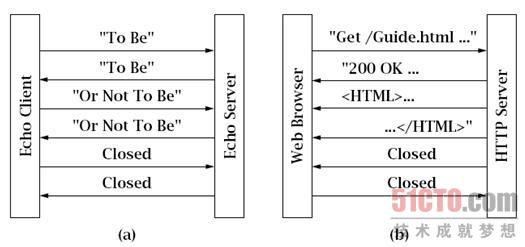
\includegraphics[scale=.8]{img/04.01.jpg}
		\caption{回显协议(a)与HTTP协议的终止(b)}
		\label{fig:echo.pt.and.http.end}
	\end{figure}

	Echo Client:回显客户端;Echo Server:回显服务器;Closed:关闭;Web Browser:网络浏览器;HTTP Server:HTTP服务器;Closed:关闭 

	实际上,客户端的关闭表示通信已经完成。HTTP协议也是一样的原理,只是它的通信终止发起者是服务器。 

	下面考虑另一种协议。假设你需要一个压缩服务器,将接收到的字节流压缩后,发回给客户端。这种情况下应该由哪一端来关闭连接呢?由于从客户端发来的字节流的长度是任意的,客户端需要关闭连接以通知服务器要压缩的字节流已经发送完毕。那么客户端应该什么时候调用close()方法呢?如果客户端在其发送完最后一个字节后立即调用套接字的close(),它将无法接收到压缩后数据的最后一些字节。或许客户端可以像回显协议那样,在接收完所有压缩后的数据才关闭连接。但不幸的是,这样一来服务器和客户端都不知道到底有多少数据要接收,因此这也不可行。我们需要一种方法来告诉连接的另一端"我已经发送完所有数据",同时还要保持接收数据的能力。 

	幸运的是套接字提供了一种实现这个功能的方法。Socket类的shutdownInput()和shutdownOutput()方法能够将输入输出流相互独立地关闭。调用shutdownInput()后,套接字的输入流将无法使用。任何没有发送的数据都将毫无提示地被丢弃,任何想从套接字的输入流读取数据的操作都将返回-1。当Socket调用shutdownOutput() 方法后,套接字的输出流将无法再发送数据,任何尝试向输出流写数据的操作都将抛出一个IOException异常。在调用shutdownOutput()之前写出的数据可能能够被远程套接字读取,之后,在远程套接字输入流上的读操作将返回-1。应用程序调用shutdownOutput()后还能继续从套接字读取数据,类似的,在调用shutdownInput()后也能够继续写数据。 

	在压缩协议中(见图4.2),客户端向服务器发送待压缩的字节,发送完成后调用shutdownOutput()关闭输出流,并从服务器读取压缩后的字节流。服务器反复地获取未压缩的数据,并将压缩后的数据发回给客户端,直到客户端执行了停机操作,导致服务器的read操作返回-1,这表示数据流的结束。然后服务器关闭连接并退出。 

	\begin{figure}[htbp]%位置选项
		\centering
		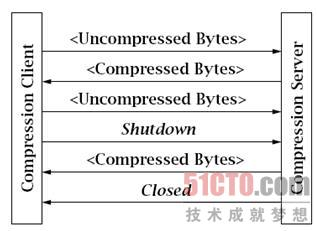
\includegraphics[scale=.8]{img/04.02.jpg}
		\caption{压缩协议终止}
		\label{fig:copose.pot.end}
	\end{figure}

	Compression Client:压缩客户端;Compression Server:压缩服务器;

	Uncompressed Bytes:未压缩字节;Compressed Bytes:已压缩字节;

	Shutdown:停机;Closed:关闭 

	在客户端调用了shutdownOutput之后,它还要从服务器读取剩余的已经压缩的字节。 

	下面的压缩客户端示例程序,CompressClient.java,实现了压缩协议的客户端。程序从命令行中指定的文件读取未压缩字节,然后将压缩后的字节写入一个新的文件。设未压缩文件名是"data",压缩后文件名是"data.gz"。注意,这个程序只适用于处理小文件,对于大文件来说其存在一个缺陷将导致死锁。(我们将在第6.2节讨论并改正这个缺陷。) 

	\lstinputlisting[language=Java,firstline=1]{src/ch04/CompressClient.java}

	1.应用程序设置和参数解析:

	2.创建套接字和打开文件:

	3.调用sendBytes()方法传输字节:

	4.接收压缩后的数据流:

	while循环反复接收压缩后的数据流并将字节写入输出文件,直到read()方法返回-1表示数据流的结束。 

	5.关闭套接字和文件流:

	6.sendBytes():

	给定一个连接到压缩服务器的套接字和一个文件输入流,从文件中读取所有未压缩的字节,并将其写入套接字的输出流。 

	获取套接字输出流:

	向压缩服务器发送未压缩字节:

	while循环从输入流读(在这个例子中是从一个文件)取数据并反复将字节发送到套接字的输出流,直到read()方法返回-1表示到达文件结尾。每一次写操作由打印到控制台的"W"指示。 

	关闭套接字输出流:

	在读取和发送完输入文件的所有字节后,关闭输出流,以通知服务器客户端已经完成了数据发送。close操作将导致服务器端的read()方法返回-1。 

	我们简单地为多线程的服务器构架写了一个协议,来实现压缩服务器。我们的协议实现,CompressProtocol.java,使用GZIP压缩算法实现了服务器端的压缩协议。服务器从客户端接收未压缩的字节,并将其写入GZIPOutputStream,它对套接字的输出流进行了包装。 

	\lstinputlisting[language=Java,firstline=1]{src/ch04/CompressProtocol.java}

	1.变量和构造函数:

	2.handleCompressClient():

	给定一个连接到压缩客户端的套接字,从客户端读取未压缩字节并将压缩后的字节写回客户端。 

	获取套接字I/O流:

	套接字的输出流包装在一个GZIPOutputStream中。写向这个流的字节序列将由GZIP算法对其进行压缩,然后再写入底层的输出流。 

	读取未压缩字节和写压缩后的字节:

	while循环从套接字输入流读取数据,并写入GZIPOutputStream,再由它将压缩后的数据写入套接字的输出流,直到接收到流结束标记。 

	刷新和关闭:

	在关闭GZIPOutputStream之前需要刷新提交可能被压缩算法缓存的字节。 

	run()方法:

	run()方法只是简单地对handleCompressClient()方法进行调用。 

	为了使用这个协议,我们对TCPEchoServerExecutor.java进行了简单的修改,创建了一个CompressProtocol实例来替代EchoProtocol实例: 

	\lstinputlisting[language=Java,firstline=147,lastline=147]{src/ch04/ThreadExample.txt}

\section{Applets} 

	Applet可以通过TCP/IP套接字在网络上进行通信,不过对于它们如何通信以及可以与谁通信有一些限制。如果没有这些限制,可信任的浏览器就可能执行有害的applet程序,例如,可能会发送欺骗邮件,或在用户使用浏览器时试图攻击其他系统,等等。这些安全性限制是由Java的安全管理器强制实施的,如果applet违法了这些限制,则将抛出SecurityException异常。通常,浏览器只允许applet与自身所在的宿主主机进行通信。这就意味着applet限制为只能与在宿主主机上执行的应用程序通信,通常是创建该applet的Web服务器。有关applet编程的安全性限制列表不属于本书的讨论范围,不过这也没多大价值,因为如果使用浏览器的用户允许的话,其默认的安全限制也可以改变。 

	假设现在需要实现一个允许用户在浏览器中输入和保存笔记的applet。由于浏览器的安全性限制阻止了applet直接向本地文件系统保存数据,因此要使用有别于本地磁盘输入输出的其他方法来保存笔记。FileClientApplet.java(见本书网站)实现了一个applet,它允许用户在一个编辑窗口中输入文本,点击"保存"按钮后,通过网络将文本复制到一个服务器上(运行在5000端口)。服务器,TCPFileServer.java(见本书网站),再将数据保存到一个文件中。它需要一个端口号(使用与applet对应的5000端口)和文件名作为参数。该服务器程序必须运行在向浏览器提供applet的Web服务器上。注意该服务器并没有任何applet特性。网页上的FileClientApplet.html文件演示了如果将applet整合到一个网页中。 

\section{结束} 

	本章中讨论了Java提供的一些访问套接字API高级特性的一些方法,以及如何使用多线程、执行器等内置功能来进行套接字编程。另外,Java还提供了一些机制(在这里没有作讨论),在TCP和UDP协议上层进行操作,并隐藏了协议开发的复杂性。例如,Java远程方法调用(Remote Method Invocation ,RMI)允许在不同主机上的Java对象相互调用彼此的方法,就像这些对象都驻留在本地一样。URL类以及其他相关类提供了一个开发Web程序的框架。还有不少标准的Java库,提供了很多各种令人惊奇的服务机制。这些机制不在本书的讨论范围之内,然而,我们建议你访问本书的网站,参考这些库的介绍并动手编写一些示例程序。 



		\chapter{NIO} 

	本章将对"New I/O"工具包的主要应用进行介绍。NIO主要包括两个部分:

	java.nio.channels包介绍了Selector和Channel抽象,java.nio包介绍了Buffer抽象。这都是一些高级的特性,有许多微妙的使用细节,因此,本章的组织结构也与前面的章节略有不同。第1节通过介绍它们所要解决的具体问题来引出NIO特性--尤其是当没有这些特性时,构建高性能服务器所面临的挑战。(如果你并不关心"为什么?"这类问题,可以直接跳过本节。)在第5.2节,我们将像前面一样展示一个(TCP)"回显"协议客户端,以介绍SocketChannel和Buffer类的使用方法,以及Channel非阻塞特性(nonblocking),这与第4.2节中介绍的阻塞特性有所不同。第5.3节中展示了一个使用了Selector,Channel和Buffer抽象服务器。

	然后我们回到主要抽象数据类型的使用细节上,各自用一小节进行介绍。最后,在第5.7节介绍了DatagramChannel类(DatagramSocket类的信道化版本)。 

\section{为什么需要NIO} 

	基本的Java套接字对于小规模系统可以很好地运行,但当涉及到要同时处理上千个客户端的服务器时,可能就会产生一些问题。其实在第4章已经可以看到一些迹象:由于创建、维护和切换线程需要的系统开销,一客户一线程方式在系统扩展性方面受到了限制。使用线程池可以节省那种系统开销,同时允许实现者利用并行硬件的优势。但对于连接生存期比较长的协议来说,线程池的大小仍然限制了系统可以同时处理的客户端数量。考虑一个在客户端之间传递消息的即时消息服务器(Instant Messaging)。客户端必须不停地连接服务器以接收即时消息,因此线程池的大小限制了系统可以同时服务的客户端总数。如果增加线程池的大小,将带来更多的线程处理开销,而不能提升系统的性能,因为在大部分的时间里客户端是处于闲置状态的。 

	如果这就是所有问题,可能NIO还不是必要的。不幸的是,在使用线程的扩展性方面还涉及一些更加难以把握的挑战。其中一个挑战就是程序员几乎不能对什么时候哪个线程将获得服务进行控制。你可以设置一个线程实例的优先级(priority)(高优先级的线程相对于低优先级的线程有优先权),但是这个优先级只是一种"建议"--下一个选择执行的线程完全取决于具体实现。因此,如果程序员想要保证某些连接优先获得服务,或想要指定一定的服务顺序,线程可能就很难做到。

	然而,有关线程的最重要的问题可能是我们至今还未提及。那是因为在"回显服务"示例程序中,每个客户端都与其他客户端相互独立,客户端之间没有交互,也不会影响服务器的状态。但是在实际情况中,大多数的服务器有一些信息(称为"状态")需要由不同的客户端同时访问或修改。例如,考虑一种允许大城市的市民保留一个小时停车位的服务。计划什么时间段由谁获得哪个停车位必须保持一致,而且,该服务必须保证同一用户在同一时间段内最多只能获得一个停车位。这些限制就要求在所有客户之间共享一些状态信息(即调度表)。这需要通过使用锁(locks)机制或其他互斥机制对依次访问状态进行严格的同步(synchronized)。否则,由于调度程序能够使不同线程上的程序段在一定程度上交错执行,如果不同线程试图同时更新调度表,它们就可能改写掉其他线程所作的修改。 

	由于需要对共享状态进行同步访问,要同时考虑到多线程服务器的正确性和高效性就变得非常困难。至于其为什么会增加复杂性已经超出了本书的讨论范围,只要进行简单的了解就足够了:使用同步机制将增加更多的系统调度和上下文切换开销,而程序员对这些开销又无法控制。由于其复杂性,一些程序员宁愿继续使用单线程(single-threaded)方法。这类服务器只用一个线程来处理所有的客户端--不是顺序处理,而是一次全部处理。这种服务器不能为任何客户端提供I/O操作的阻塞等待,而必须排他地使用非阻塞式(nonblocking)I/O。回顾前面所介绍的非阻塞式I/O,我们需要指定调用I/O方法时的最长阻塞时间(包括0)。 

	在第4章我们见过一个为accept操作设置超时(通过使用ServerSocket类的setSoTimeout()方法)的例子。当在ServerSocket实例上调用accept()方法时,如果有一个新的连接请求正在等待,accept()方法则立即返回;否则该方法将阻塞等待,直到有新的连接请求到来或计时器超时,这取决于哪个先发生(有连接请求或超时)。这里只有一个线程来处理多个连接。不幸的是,这种方法要求我们不断地轮询(poll)所有I/O源,而这种"忙等(busy waiting)"方法又会引入很多系统开销,因为程序要在连接之间反复循环,却又发现什么都不用做。 

	我们需要一种方法来一次轮询一组客户端,以查找哪个客户端需要服务。这正是NIO中将要介绍的Selector和Channel抽象的关键点。一个Channel实例代表了一个"可轮询的(pollable)"I/O目标,如套接字(或一个文件、设备等)。Channel能够注册一个Selector类的实例。Selector的select()方法允许你询问"在一组信道中,哪一个当前需要服务(即,被接受,读或写)?"大量的细节将在后文中介绍,但这就是使用Selector和Channel的基本动机。这两个类都包含在java.nio.channels包中。 

	NIO中将介绍的另一个主要特性是Buffer类。就像selector和channel为一次处理多个客户端的系统开销提供了更高级的控制和可预测性,Buffer则提供了比Stream抽象更高效和可预测的I/O。 Stream抽象好的方面是隐藏了底层缓冲区的有限性,提供了一个能够容纳任意长度数据的容器的假象。坏的方面是要实现这样一个假象,要么会产生大量的内存开销,要么会引入大量的上下文切换,甚至可能两者都有。在使用线程时,这些开销都隐藏在了具体实现中,因此也失去了对其的可控性和可预测性。这种方法使编写程序变得容易,但要调整它们的性能则变得更困难。不幸的是,如果要使用Java的Socket抽象,流就是唯一的选择。 

	这就是为什么要把channel设计为使用Buffer实例来传递数据。Buffer抽象代表了一个有限容量(finite-capacity)的数据容器--其本质是一个数组,由指针指示了在哪存放数据和从哪读取数据。使用Buffer有两个主要好处。第一,与读写缓冲区数据相关联的系统开销暴露给了程序员。例如,如果想要向缓冲区存入数据,但又没有足够的空间时,就必须采取一些措施来获得空间(即,移出一些数据,或移开已经在那个位置的数据来获得空间,或者创建一个新的实例)。这意味着需要额外的工作,但是你(程序员)可以控制它什么时候发生,如何发生,以及是否发生。一个聪明的程序员如果清楚地了解了应用程序的需求,就那能通过权衡这些选择来降低系统开销。第二,一些对Java对象的特殊Buffer映射操作能够直接操作底层平台的资源(例如,操作系统的缓冲区)。这些操作节省了在不同地址空间中复制数据的开销--这在现代计算机体系结构中是开销很大的操作。 

\section{与Buffer一起使用Channel} 

	如前文所述,Channel实例代表了一个与设备的连接,通过它可以进行输入输出操作。实际上Channel的基本思想与我们见过的普通套接字非常相似。对于TCP协议,可以使用ServerSocketChannel和SocketChannel。还有一些针对其他设备的其他类型信道(如,FileChannel),尽管我们在后文中不会再提及,这里介绍的大部分内容对于它们同样适用。信道(channel)和套接字(socket)之间的不同点之一,可能是信道通常要调用静态工厂方法来获取实例: 

	\lstinputlisting[language=Java,firstline=1,lastline=2]{src/ch05/TCPEchoClientNonblocking.txt}

	Channel使用的不是流,而是缓冲区来发送或读取数据。Buffer类或其任何子类的实例都可以看作是一个定长的Java基本数据类型元素序列。与流不同,缓冲区有固定的、有限的容量,并由内部(但可以被访问)状态记录了有多少数据放入或取出,就像是有限容量的队列一样。Buffer是一个抽象类,只能通过创建它的子类来获得Buffer实例,而每个子类都设计为用来容纳一种Java基本数据类型(boolean除外)。因此,这些实例分别为FloatBuffer,或IntBuffer,或ByteBuffer,等等(ByteBuffer是这些实例中最灵活的,并将在后面很多例子中用到)。在channel中使用Buffer实例通常不是使用构造函数创建的,而是通过调用allocate()方法创建指定容量的Buffer实例, 

	\lstinputlisting[language=Java,firstline=5,lastline=5]{src/ch05/TCPEchoClientNonblocking.txt}

	或通过包装一个已有的数组来创建: 

	\lstinputlisting[language=Java,firstline=6,lastline=6]{src/ch05/TCPEchoClientNonblocking.txt}

	NIO的强大功能部分来自于channel的非阻塞特性。回顾前面介绍的内容可以知道,套接字的某些操作可能会无限期地阻塞。例如,对accept()方法的调用可能会因为等待一个客户端连接而阻塞;对read()方法的调用可能会因为没有数据可读而阻塞,直到连接的另一端传来新的数据。总的来说,创建/接收连接或读写数据等I/O调用,都可能无限期地阻塞等待,直到底层的网络实现发生了什么。慢速的、有损耗的网络,或仅仅是简单的网络故障都可能导致任意时间的延迟。然而不幸的是,在调用一个方法之前无法知道其是否会阻塞。NIO的channel抽象的一个重要特征就是可以通过配置它的阻塞行为,以实现非阻塞式的信道。 

	\lstinputlisting[language=Java,firstline=8,lastline=8]{src/ch05/TCPEchoClientNonblocking.txt}

	在非阻塞式信道上调用一个方法总是会立即返回。这种调用的返回值指示了所请求的操作完成的程度。例如,在一个非阻塞式ServerSocketChannel上调用accept()方法,如果有连接请求在等待,则返回客户端SocketChannel,否则返回null。下面我们来创建一个非阻塞式TCP回显客户端。可能阻塞的I/O操作包括建立连接,读和写。通过使用非阻塞式信道,这些操作都将立即返回。我们必须反复调用这些操作,直到所有I/O操作都成功完成。 


	\lstinputlisting[language=Java,firstline=1]{src/ch05/TCPEchoClientNonblocking.java}

	1.获取并转换参数:

	2. 创建非阻塞式SocketChannel:

	3.连接服务器:

	由于该套接字是非阻塞式的,因此对connect()方法的调用可能会在连接建立之前返回,如果在返回前已经成功建立了连接,则返回true,否则返回false。对于后一种情况,任何试图发送或接收数据的操作都将抛出NotYetConnectedException异常,因此,我们通过持续调用finishConnect()方法来"轮询"连接状态,该方法在连接成功建立之前一直返回false。打印操作演示了在等待连接建立的过程中,程序还可以执行其他任务。不过,这种忙等的方法非常浪费系统资源,这里这样做只是为了演示该方法的使用。 

	4.创建读写缓冲区:

	我们分别使用了两种方法来创建将要用来读写数据的ByteBuffer实例。一是通过包装包含了要发送数据的byte[]数组,另一个方法是调用allocate()方法,创建具有与前面byte[]数组大小相同缓冲区的ByteBuffer实例。 

	5.反复循环直到发送和接收完所有字节:

	只要输出缓冲区中还留有数据,就调用write()方法。对read()方法的调用不会阻塞等待,但是当没有数据可读时该方法将返回0。这里,打印语句再次举例说明了在等待通信完成的过程中,程序可以执行其他任务。 

	6.打印接收到的数据:

	7.关闭信道:

	与套接字类似,信道在完成其任务后也需要关闭。 

\section{Selector} 

	如本章第1节中提到的,Selector类可用于避免使用非阻塞式客户端中很浪费资源的"忙等"方法。例如,考虑一个即时消息服务器。可能有上千个客户端同时连接到了服务器,但在任何时刻都只有非常少量的(甚至可能没有)消息需要读取和分发。这就需要一种方法阻塞等待,直到至少有一个信道可以进行I/O操作,并指出是哪个信道。NIO的选择器就实现了这样的功能。一个Selector实例可以同时检查(如果需要,也可以等待)一组信道的I/O状态。用专业术语来说,选择器就是一个多路开关选择器,因为一个选择器能够管理多个信道上的I/O操作。 

	要使用选择器,需要创建一个Selector实例(使用静态工厂方法open())并将其注册(register)到想要监控的信道上(注意,这要通过channel的方法实现,而不是使用selector的方法)。最后,调用选择器的select()方法。该方法会阻塞等待,直到有一个或更多的信道准备好了I/O操作或等待超时。select()方法将返回可进行I/O操作的信道数量。现在,在一个单独的线程中,通过调用select()方法就能检查多个信道是否准备好进行I/O操作。如果经过一段时间后仍然没有信道准备好,select()方法就返回0,并允许程序继续执行其他任务。 

	下面来看一个例子。假设我们想要使用信道和选择器来实现一个回显服务器,并且不使用多线程和忙等。为了使不同协议都能方便地使用这个基本的服务模式,我们把信道中与具体协议相关的处理各种I/O的操作(接收,读,写)分离了出来。TCPProtocol定义了通用TCPSelectorServer类与特定协议之间的接口,包括三个方法,每个方法代表了一种I/O型式。当有信道准备好I/O操作时,服务器只需要调用相应的方法即可。 

	\lstinputlisting[language=Java,firstline=1]{src/ch05/TCPProtocol.java}

	在服务器端创建一个选择器,并将其与每个侦听客户端连接的套接字所对应的ServerSocketChannel注册在一起。然后进行反复循环,调用select()方法,并调用相应的操作器例程对各种类型的I/O操作进行处理。 

	\lstinputlisting[language=Java,firstline=1]{src/ch05/TCPServerSelector.java}

	1.设置:

	验证至少有一个参数,创建一个Selector实例。 

	2.为每个端口创建一个ServerSocketChannel:

	创建一个ServerSocketChannel实例:

	使其侦听给定端口:

	需要获得底层的ServerSocket,并以端口号作为参数调用其bind()方法。任何超出适当数值范围的参数都将导致抛出IOException异常。 

	配置为非阻塞模式:

	只有非阻塞信道才可以注册选择器,因此需要将其配置为适当的状态。 

	为信道注册选择器:

	在注册过程中指出该信道可以进行"accept"操作。 

	3.创建协议操作器:

	为了访问回显协议中的操作方法,创建了一个EchoSelectorProtocol实例。该实例包含了需要用到的方法。 

	4.反复循环,等待I/O,调用操作器:

	选择:

	这个版本的select()方法将阻塞等待,直到有准备好I/O操作的信道,或直到发生了超时。该方法将返回准备好的信道数。返回0表示超时,这时程序将打印一个点来标记经过的时间和迭代次数。 

	获取所选择的键集:

	调用selectedKeys()方法返回一个Set实例,并从中获取一个Iterator。该集合中包含了每个准备好某一I/O操作的信道的SelectionKey(在注册时创建)。 

	在键集上迭代,检测准备好的操作:第42-58行 

	对于每个键,检查其是否准备好进行accep()操作,是否可读或可写,并调用相应的操作器方法对每种情况进行指定的操作。 

	从集合中移除键:

	由于select()操作只是向Selector所关联的键集合中添加元素,因此,如果不移除每个处理过的键,它就会在下次调用select()方法是仍然保留在集合中,而且可能会有无用的操作来调用它。 

	TCPServerSelector的大部分内容都与协议无关,只有协议赋值那一行代码是针对的特定协议。所有协议细节都包含在了TCPProtocol接口的具体实现中。EchoSelectorProtocol类就实现了该回显协议的操作器。你可以轻松地为自其他协议编写自己的操作器,或在我们的回显协议操作器上进行改进。 

	\lstinputlisting[language=Java,firstline=1]{src/ch05/EchoSelectorProtocol.java}

	1.声明实现TCPProtocol接口:

	2.成员变量和构造函数:

	每个实例都包含了将要为每个客户端信道创建的缓冲区大小。 

	3. handleAccept(): 

	从键中获取信道,并接受连接:

	channel()方法返回注册时用来创建键的Channel。(我们知道该Channel是一个ServerSocketChannel,因为这是我们注册的惟一一种支持"accept"操作的信道。)accept()方法为传入的连接返回一个SocketChannel实例。 

	设置为非阻塞模式:

	再次提醒,这里无法注册阻塞式信道。 

	为信道注册选择器:

	可以通过SelectionKey类的selector()方法来获取相应的Selector。我们根据指定大小创建了一个新的ByteBuffer实例,并将其作为参数传递给register()方法。它将作为附件,与register()方法所返回的SelectionKey实例相关联。(在此我们忽略了返回的键,但当信道准备好读数据的I/O操作时,可以通过选出的键集对其进行访问。) 

	4. handleRead():

	获取键关联的信道:

	根据其支持数据读取操作可知,这是一个SocketChannel。 

	获取键关联的缓冲区:第25行 

	连接建立后,有一个ByteBuffer附加到该SelectionKey实例上。 

	从信道中读数据: 

	检查数据流的结束并关闭信道:

	如果read()方法返回-1,则表示底层连接已经关闭,此时需要关闭信道。关闭信道时,将从选择器的各种集合中移除与该信道关联的键。 

	如果接收完数据,将其标记为可写:

	注意,这里依然保留了信道的可读操作,虽然缓冲区中可能已经没有剩余空间了。 

	5. handleWrite():

	获取包含数据的缓冲区:

	附加到SelectionKey上的ByteBuffer包含了之前从信道中读取的数据。 

	准备缓冲区的写操作:第42行 

	Buffer的内部状态指示了在哪里放入下一批数据,以及缓冲区还剩多少空间。flip()方法用来修改缓冲区的内部状态,以指示write()操作从什么地方获取数据,以及还有剩余多少数据。(下一章将对其进行详细介绍。)该方法的作用是使写数据的操作开始消耗由读操作产生的数据。 

	获取信道:

	向信道写数据:

	如果缓冲区为空,则标记为不再写数据:

	如果缓冲区中之前接收的数据已经没有剩余,则修改该键关联的操作集,指示其只能进行读操作。 

	压缩缓冲区:

	如果缓冲区中还有剩余数据,该操作则将其移动到缓冲区的前端,以使下次迭代能够读入更多的数据(第5.4.5节将对这个操作的语义进行详细介绍)。在任何情况下,该操作都将重置缓冲区的状态,因此缓冲区又变为可读。注意,除了在handleWrite()方法内部,与信道关联的缓冲区始终是设置为可读的。 

	现在我们已经准备好对三大NIO抽象的细节进行深入研究了。 

\section{Buffer详解}

	如你所见,在NIO中,数据的读写操作始终是与缓冲区相关联的。Channel将数据读入缓冲区,然后我们又从缓冲区访问数据。写数据时,首先将要发送的数据按顺序填入缓冲区。基本上,缓冲区只是一个列表,它的所有元素都是基本数据类型(通常为字节型)。缓冲区是定长的,它不像一些类那样可以扩展容量(例如,List,StringBuffer等)。注意,ByteBuffer是最常用的缓冲区,因为:

	1)它提供了读写其他数据类型的方法。

	2)信道的读写方法只接收ByteBuffer。

	那么其他类型的信道,如IntBuffer,DoubleBuffer等的优点在哪呢?稍安毋躁!答案将在第5.4.6节揭晓。 


	\subsection{Buffer索引}

		缓冲区不仅仅是用来存放一组元素的列表。在读写数据时,它有内部状态来跟踪缓冲区的当前位置,以及有效可读数据的结束位置等。为了实现这些功能,每个缓冲区维护了指向其元素列表的4个索引,如表5.1所示。(不久我们将看到如何使用缓冲区的各种方法来修改索引值。) 

		\begin{table}[htbp]
			\caption{缓冲区内部状态}
			\label{tab:state.of.buffer}
			\centering
			\begin{tabular}{lll}
				\hline
					索引 & 描述   & 存取器/修改器/用法 \\
				\hline
					capacity & 缓冲区中的元素总数(不可修改) & int capacity() \\
				\hline
					\multirow{2}{*}{position } & 
					\multirow{2}{*}{下一个要读/写的元素(从0开始)} & 
					int position() \\

					& & Buffer position(int newPosition) \\
				\hline
					\multirow{2}{*}{ limit} & 
					\multirow{2}{*}{ 第一个不可读/写元素} & 
					int limit() \\

					& & Buffer limit(int newLimit) \\
				\hline
					\multirow{2}{*}{mark} & 
					\multirow{2}{*}{用户选定的position的前一个位置,或0}  & 
					Buffer mark() \\

					&  & Buffer reset() \\
				\hline
			\end{tabular}
		\end{table}

		position和limit之间的距离指示了可读取/存入的字节数。Java中提供了两个方便的方法来计算这个距离。 

		ByteBuffer: 剩余字节 

		\lstinputlisting[language=Java,firstline=11,lastline=12]{src/ch05/TCPEchoClientNonblocking.txt}

		当缓冲区至少还有一个元素时,hasRemaining()方法返回true,remaining()方法返回剩余元素的个数。 

		在这些变量中,以下关系保持不变: 

		0 ≤ mark ≤ position ≤ limit ≤ capacity 

		mark变量的值"记录"了一个将来可返回的位置,reset()方法则将position的值还原成上次调用mark()方法后的position值(除非这样做会违背上述的不变关系)。 

	\subsection{创建Buffer} 

		通常使用分配空间或包装一个现有的基本类型数组来创建缓冲区。创建ByteBuffer的静态工厂方法,以及相应的capacity,position,和limit的初始值见表5.2。所有新创建的Buffer实例都没有定义其mark值,在调用mark()方法前,任何试图使用reset()方法来设置position的值的操作都将抛出InvalidMarkException异常。 

		要分配一个新的实例,只需要简单地调用想要创建的缓冲区类型的allocate()静态方法,并指定元素的总数: 

		\lstinputlisting[language=Java,firstline=16,lastline=17]{src/ch05/TCPEchoClientNonblocking.txt}

		\begin{table}[htbp]
			\caption{ByteBuffer创建方法}
			\label{tab:create.byte.buffer}
			\centering
			\begin{tabular}{llll}
				\hline
					方法 & Capacity & Position & Limit \\
				\hline
					ByteBuffer allocate(int capacity)                     & capacity     & 0      & capacity \\
					ByteBuffer allocateDirect(int capacity)               & capacity     & 0      & capacity \\
					ByteBuffer wrap(byte[] array)                         & array.length & 0      & array.length \\
					ByteBuffer wrap(byte[] array, int offset, int length) & array.length & offset & offset + length \\
				\hline
			\end{tabular}
		\end{table}

		在上面代码中,byteBuf分配了20个字节,dblBuf分配了5个Java的double型数据。这些缓冲区都是定长的,因此无法扩展或缩减它们的容量。如果发现刚创建的缓冲区容量太小,惟一的选择就是重新创建一个大小合适的缓冲区。 

		还可以通过调用wrap()静态方法,以一个已有的数组为参数,来创建缓冲区: 

		\lstinputlisting[language=Java,firstline=21,lastline=24]{src/ch05/TCPEchoClientNonblocking.txt}

		通过包装的方法创建的缓冲区保留了被包装数组内保存的数据。实际上,wrap()方法只是简单地创建了一个具有指向被包装数组的引用的缓冲区,该数组称为后援数组。对后援数组中的数据做的任何修改都将改变缓冲区中的数据,反之亦然。如果我们为wrap()方法指定了偏移量(offset)和长度(length),缓冲区将使用整个数组为后援数组,同时将position和limit的值初始化为偏移量(offset)和偏移量+长度(offset+length)。在偏移量之前和长度之后的元素依然可以通过缓冲区访问。 

		使用分配空间的方式来创建缓冲区其实与使用包装的方法区别不大。惟一的区别是allocate()方法创建了自己的后援数组。在缓冲区上调用array()方法即可获得后援数组的引用。通过调用arrayOffset()方法,甚至还可以获取缓冲区中第一个元素在后援数组中的偏移量。使用wrap()方法和非零偏移量参数创建的缓冲区,其数组偏移量依然是0。 

		到目前为止,我们实现的所有缓冲区都将数据存放在Java分配的后援数组中。通常,底层平台(操作系统)不能使用这些缓冲区进行I/O操作。操作系统必须使用自己的缓冲区来进行I/O,并将结果复制到缓冲区的后援数组中。这些复制过程可能非常耗费系统资源,尤其是在有很多读写需求的时候。Java的NIO提供了一种直接缓冲区(direct buffers)来解决这个问题。使用直接缓冲区,Java将从平台能够直接进行I/O操作的存储空间中为缓冲区分配后援存储空间,从而省略了数据的复制过程。这种低层的、本地的I/O通常在字节层进行操作,因此只能为 ByteBuffer进行直接缓冲区分配。 

		\lstinputlisting[language=Java,firstline=31,lastline=31]{src/ch05/TCPEchoClientNonblocking.txt}

		通过调用isDirect()方法可以查看一个缓冲区是否是直接缓冲区。由于直接缓冲区没有后援数组,在它上面调用array()或arrayOffset()方法都将抛出UnsupportedOperationException异常。在考虑是否使用直接缓冲区时需要牢记几点。首先,要知道调用allocateDirect()方法并不能保证能成功分配直接缓冲区--有的平台或JVM可能不支持这个操作,因此在尝试分配直接缓冲区后必须调用isDirect()方法进行检查。其次,要知道分配和销毁直接缓冲区通常比分配和销毁非直接缓冲区要消耗更多的系统资源,因为直接缓冲区的后援存储空间通常存在与JVM之外,对它的管理需要与操作系统进行交互。所以,只有当需要在很多I/O操作上长时间使用时,才分配直接缓冲区。实际上,在相对于非直接缓冲区能明显提高系统性能时,使用直接缓冲区是个不错的主意。 

	\subsection{存储和接收数据}

		只要有了缓冲区,就可以用它来存放数据了。作为数据的"容器",缓冲区既可用来输入也可用来输出。这一点就与流不同,流只能向一个方向传递数据。使用put()方法可以将数据放入缓冲区,使用get()方法则可以从缓冲区获取数据。信道的read()方法隐式调用了给定缓冲区的put(),而其write()方法则隐式调用了缓冲区的get()方法。下面展示了ByteBuffer的get()和put()方法,当然,其他类型的缓冲区也有类似的方法。 

		ByteBuffer: 获取和存放字节 

		相对位置: 

		\lstinputlisting[language=Java,firstline=35,lastline=41]{src/ch05/TCPEchoClientNonblocking.txt}

		绝对位置: 

		\lstinputlisting[language=Java,firstline=45,lastline=46]{src/ch05/TCPEchoClientNonblocking.txt}

		有两种类型的get()和put():基于相对位置和基于绝对位置。基于相对位置的版本根据position的当前值,从"下一个"位置读取或存放数据,然后根据数据量给position增加适当的值(即,单字节形式增加1, 数组形式增加array.length, 数组/偏移量/长度形式则增加length)。也就是说,每次调用put()方法,都是在缓冲区中的已有元素后面追加数据,每次调用get()方法,都是读取缓冲区的后续元素。不过,如果这些操作会导致position的值超出limit的限制,get()方法将抛出BufferUnderflowException异常,put()方法将抛出BufferOverflowException异常。例如,如果传给get()方法的目标数组长度大于缓冲区的剩余空间大小,get()方法将抛出BufferUnderflowException异常,部分数据的get/put是不允许的。基于绝对位置的get()和put()以指定的索引位置为参数,从该位置读取数据或向该位置写入数据。绝对位置形式的get和put不会改变position的值。如果给定的索引值超出了limit的限制,它们将抛出IndexOutOfBoundsException异常。 

		除了字节类型外,ByteBuffer类还提供了其他类型数据的相当位置和绝对位置的get/put方法。这样一来,就有点像DataOutputStream了。 

		ByteBuffer: 读取和存放Java多字节基本数据 

		\lstinputlisting[language=Java,firstline=51,lastline=54]{src/ch05/TCPEchoClientNonblocking.txt}

		其中"<Type>"代表Char,Double,Int,Long,Short之一,而"<type>"代表char,double,int,long,short之一。 

		每次调用基于相对位置的put()或get()方法,都将根据特定参数类型的长度增加position的值:short加2,int加4,等。不过,如果这样做会导致position的值超出limit的限制,get()和put()方法将分别抛出BufferUnderflowException和BufferOverflowException异常:get和put不允许只对部分数据进行操作。发生了下溢/上溢(under/overflow)时,position的值不变。 

		可能你已经注意到,很多get/put方法都返回一个ByteBuffer。实际上它们返回的就是调用它们的那个ByteBuffer。这样做可以实现链式调用(call chaining),即第一次调用的结果可以直接用来进行后续的方法调用。例如,可以像下面那样将整数1和2存入ByteBuffer实例 myBuffer中: 

		\lstinputlisting[language=Java,firstline=57,lastline=57]{src/ch05/TCPEchoClientNonblocking.txt}

		回顾第3章的内容我们知道,多字节数据类型有一个字节顺序,称为big-endian或little-endian。Java默认使用big-endian。通过使用内置的\verb|ByteOrder.BIG_ENDIAN|和\verb|ByteOrder.LITTLE_ENDIAN|实例,可以获取和设定多字节数据类型写入字节缓冲区时的字节顺序。 

		ByteBuffer: 缓冲区中的字节顺序 

		\lstinputlisting[language=Java,firstline=61,lastline=62]{src/ch05/TCPEchoClientNonblocking.txt}

		第一个方法以ByteOrder常量的形式返回缓冲区的当前字节顺序。第二个方法用来设置写多字节数据时的字节顺序。 

		下面来看一个使用字节顺序的例子: 

		\lstinputlisting[language=Java,firstline=71,lastline=75]{src/ch05/TCPEchoClientNonblocking.txt}

		看了这些有关字节顺序的讨论,你可能希望知道自己的处理器是什么字节顺序,ByteOrder定义了一个方法来解答这个问题: 

		ByteOrder: 查找字节顺序 

		\lstinputlisting[language=Java,firstline=81,lastline=83]{src/ch05/TCPEchoClientNonblocking.txt}

		nativeOrder()方法返回常量\verb|BIG_ENDIAN|或\verb|LITTLE_ENDIAN|之一。 
	
	\subsection{准备Buffer:clear(),flip(),和rewind()}

		在使用缓冲区进行输入输出数据之前,必须确定缓冲区的position,limit都已经设置了正确的值。下面考虑一个容量为7的CharBuffer实例,并已经连续调用了put()或read()方法: 

		“\verb|^|”表示position,“\verb|*|”表示limit。

		\lstinputlisting[language=Java,firstline=91,lastline=95]{src/ch05/TCPEchoClientNonblocking.txt}

		如果现在想用这个缓冲区进行信道的写操作,由于write()方法将从position指示的位置开始读取数据,在limit指示的位置停止,因此在进行写操作前,先要将limit的值设为position的当前值,再将position的值设为0。 

		\lstinputlisting[language=Java,firstline=98,lastline=102]{src/ch05/TCPEchoClientNonblocking.txt}

		这种情况我们可以自己处理,不过,幸运的是Java已经提供了一些便利的方法来完成这些工作,见表5.3。 

		注意,这些方法不会改变缓冲区中的数据,只是改变缓冲区的索引。clear()方法将position设置为0,并将limit设置为等于capacity,从而使缓冲区准备好从缓冲区的put操作或信道的读操作接收新的数据。 

		\lstinputlisting[language=Java,firstline=105,lastline=109]{src/ch05/TCPEchoClientNonblocking.txt}

		\begin{table}[htbp]
			\caption{ByteBuffer实例的方法}
			\label{tab:fun.of.byte.buffer}
			\centering
			\begin{tabular}{lllll}
				\hline
					\multirow{2}{*}{ByteBuffer方法} & \multirow{2}{*}{准备Buffer以实现}  & \multicolumn{3}{c}{结果值}   \\
						        					&                                    & Position & Limit     & Mark  \\
				\hline
					ByteBuffer clear()              & 将数据read()/put()进缓冲区         & 0        & capacity  & 未定义 \\
					ByteBuffer flip()               & 从缓冲区write()/get()              & 0        & position  & 未定义 \\
					ByteBuffer rewind()             & 从缓冲区rewrite()/get()            & 0        & unchanged & 未定义 \\
				\hline
			\end{tabular}
		\end{table}

		后续的put()/read()调用,将数据从第一个元素开始填入缓冲区,直到填满了limit所指定的限制,其值等于capacity的值。 

		\lstinputlisting[language=Java,firstline=128,lastline=130]{src/ch05/TCPEchoClientNonblocking.txt}

		虽然名字是clear(),但它实际上不会改变缓冲区中的数据,而只是简单地重置了缓冲区的主要索引值。考虑一个最近使用put()或read()存入了数据的缓冲区,其position值指示了不包含有效字符的第一个元素位置。 

		\lstinputlisting[language=Java,firstline=112,lastline=116]{src/ch05/TCPEchoClientNonblocking.txt}

		flip()方法用来将缓冲区准备为数据传出状态,这通过将limit设置为position的当前值,再将 position的值设为0来实现: 

		\lstinputlisting[language=Java,firstline=119,lastline=123]{src/ch05/TCPEchoClientNonblocking.txt}

		后续的get()/write()调用将从缓冲区的第一个元素开始检索数据,直到到达limit指示的位置。下面是使用flip()方法的例子: 

		\lstinputlisting[language=Java,firstline=135,lastline=140]{src/ch05/TCPEchoClientNonblocking.txt}

		假设在写出缓冲区的所有数据后,你想回到缓冲区的开始位置再重写一次相同的数据(例如,想要将同样的数据发送给另一个信道)。rewind()方法将position设置为0,并使mark值无效。这很像flip()方法的操作,只是limit的值没变。这些操作什么时候会有用呢?当你想要将在网络上发送的所有数据都写入日志时就会用到: 

		\lstinputlisting[language=Java,firstline=141,lastline=147]{src/ch05/TCPEchoClientNonblocking.txt}

	\subsection{压缩Buffer中的数据}

		compact()方法将 position与limit之间的元素复制到缓冲区的开始位置,从而为后续的put()/read()调用让出空间。position的值将设置为要复制的数据的长度,limit的值将设置为capacity,mark则变成未定义。考虑在下面的缓冲区调用compact()前的状态: 

		\lstinputlisting[language=Java,firstline=151,lastline=155]{src/ch05/TCPEchoClientNonblocking.txt}

		下面是调用compact()后的状态: 

		\lstinputlisting[language=Java,firstline=159,lastline=163]{src/ch05/TCPEchoClientNonblocking.txt}

		为什么要使用这个操作呢?假设你有一个缓冲区要写数据。回顾前面的内容我们知道,对write()方法的非阻塞调用只会写出其能够发送的数据,而不会阻塞等待所有数据发送完。因此write()方法不一定会将缓冲区中的所有元素都发送出去。又假设现在要调用read()方法,在缓冲区中没有发送的数据后面读入新数据。处理方法之一就是简单地设置position = limit和limit = capacity。当然,在读入新数据后,再次调用write()方法前,还需要将这些值还原。这样做有个问题即缓冲区的空间最终将消耗殆尽,如上图中,只剩下一个元素位置可以再存入一个字节。此外,缓冲区前面的空间又被浪费掉了。这就是compact()方法要解决的问题。在调用write()方法后和添加新数据的read()方法前调用compact()方法,则将所有"剩余"的数据移动到缓冲区的开头,从而为释放最大的空间来存放新数据。 

		\lstinputlisting[language=Java,firstline=171,lastline=178]{src/ch05/TCPEchoClientNonblocking.txt}

		注意,如在本章开始已经提到的,复制数据是一个非常耗费系统资源的操作,因此要保守地使用compact()方法。 

	\subsection{Buffer透视:duplicate(),slice()等} 

		NIO提供了多种方法来创建一个与给定缓冲区共享内容的新缓冲区,这些方法对元素的处理过程各有不同。基本上,这种新缓冲区有自己独立的状态变量(position,limit,capacity和mark),但与原始缓冲区共享了同一个后援存储空间。任何对新缓冲区内容的修改都将反映到原始缓冲区上。可以将新缓冲区看作是从另一个角度对同一数据的透视。表5.4列出了相关的方法。 

		duplicate()方法用于创建一个与原始缓冲区共享内容的新缓冲区。新缓冲区的position,limit,mark和capacity都初始化为原始缓冲区的索引值,然而,它们的这些值是相互独立的。 

		\begin{table}[htbp]
			\caption{在Buffer上创建不同透视的方法}
			\label{tab:diff.view.on.buffer}
			\centering
			\begin{tabular}{lllll}
				\hline
					\multirow{2}{*}{ByteBuffer方法} & \multirow{2}{*}{Capacity}  & \multicolumn{3}{c}{新缓冲区的初始值}   \\
						        					&                                    & Position & Limit     & Mark  \\
				\hline
					ByteBuffer duplicate()        & capacity      & position & limit         & mark   \\
					ByteBuffer slice()            & remaining()   & 0        & remaining()   & 未定义 \\
					ByteBuffer asReadOnlyBuffer() & capacity      & position & limit         & mark   \\
					CharBuffer asCharBuffer()     & remaining()/2 & 0        & remaining()/2 & 未定义 \\
					DoubleBuffer asDoubleBuffer() & remaining()/8 & 0        & remaining()/8 & 未定义 \\
					FloatBuffer asFloatBuffer()   & remaining()/4 & 0        & remaining()/4 & 未定义 \\
					IntBuffer asIntBuffer()       & remaining()/4 & 0        & remaining()/4 & 未定义 \\
					LongBuffer asLongBuffer()     & remaining()/8 & 0        & remaining()/8 & 未定义 \\
					ShortBuffer asShortBuffer()   & remaining()/2 & 0        & remaining()/2 & 未定义 \\
				\hline
			\end{tabular}
		\end{table}

		由于共享了内容,对原始缓冲区或任何复本所做的改变在所有复本上都可见。下面回到前面的例子,假设要将在网络上发送的所有数据都写进日志。 

		\lstinputlisting[language=Java,firstline=181,lastline=186]{src/ch05/TCPEchoClientNonblocking.txt}

		注意,使用了缓冲区复制操作,向网络写数据和写日志就可以在不同的线程中并行进行。 

		slice()方法用于创建一个共享了原始缓冲区子序列的新缓冲区。新缓冲区的position值是0,而其limit和capacity的值都等于原始缓冲区的limit和position的差值。slice()方法将新缓冲区数组的offset值设置为原始缓冲区的position值,然而,在新缓冲区上调用array()方法还是会返回整个数组。 

		Channel在读写数据时只以ByteBuffer为参数,然而我们可能还对使用其他基本类型的数据进行通信感兴趣。ByteBuffer能够创建一种独立的"视图缓冲区(view buffer)",用于将ByteBuffer的内容解释成其他基本类型(如CharBuffer)。这样就可以从该缓冲区中读取(写入数据是可选操作)新类型的数据。新缓冲区与原始缓冲区共享了同一个后援存储空间,因此,在任一缓冲区上的修改在新缓冲区和原始缓冲区上都可以看到。新创建的视图缓冲区的position值为0,其内容从原始缓冲区的position所指位置开始。这与slice()操作非常相似。不过,由于视图缓冲区操作的是多字节元素,新缓冲区的capacity和limit的值等于剩余总字节数除以每个该类型元素对应的字节数(例如,创建DoubleBuffer时则除以8)。 

		下面来看一个例子。假设通过某个Channel接收到一条消息,该消息由一个单独字节,后跟大量big-endian顺序的双字节整数(如short型)组成。由于该消息是通过Channel送达的,它一定在一个ByteBuffer中,在此为buf。消息的第一个字节包含了消息中双字节整数的数量。你可能要调用第一个字节指定次数的buf.getShort()方法,或者你可以一次获取所有的整数,如下所示: 

		\lstinputlisting[language=Java,firstline=191,lastline=199]{src/ch05/TCPEchoClientNonblocking.txt}

		asReadOnlyBuffer()方法的功能与duplicate()方法相似,只是任何会修改新缓冲区内容的方法都将抛出ReadOnlyBufferException异常。包括各种型式的put(),compact()等,甚至连在缓冲区上调用无方向性的array()和arrayOffset()方法也会抛出这个异常。当然,对产生这个只读缓冲区的非只读缓冲区进行的任何修改,仍然会与新的只读缓冲区共享。就像用duplicate()创建的缓冲区一样,只读缓冲区也有独立的缓冲区状态变量。可以使用isReadOnly()方法来检查一个缓冲区是否是只读的。如果原缓冲区已经是只读的,调用duplicate()或slice()方法也将创建新的只读缓冲区。 

	\subsection{字符编码}

		回顾第3章介绍的内容我们知道,字符是由字节序列进行编码的,而且在字节序列与字符集合之间有各种映射(称为字符集)方式。NIO缓冲区的另一个用途是在各种字符集之间进行转换。要使用这个功能,还需要了解java.nio.charset包中另外两个类(在第3章中我们已经介绍了Charset类):CharsetEncoder和CharsetDecoder类。 

		要进行编码,需要使用一个Charset实例来创建一个编码器并调用encode方法: 

		\lstinputlisting[language=Java,firstline=201,lastline=203]{src/ch05/TCPEchoClientNonblocking.txt}

		要进行解码,需要使用Charset实例来创建一个解码器,并调用decode方法: 

		\lstinputlisting[language=Java,firstline=206,lastline=207]{src/ch05/TCPEchoClientNonblocking.txt}

		虽然这种方法能够正常工作,但当需要进行多次编码时,效率就会变得较低。例如,每次调用encode/decode方法都会创建一个新Byte/CharBuffer实例。其他导致低效率的地方与编码器的创建和操作有关。 

		\lstinputlisting[language=Java,firstline=211,lastline=222]{src/ch05/TCPEchoClientNonblocking.txt}

		encode()方法将给定CharBuffer转换为一个字节序列,并将其写入给定的缓冲区。如果缓冲区太小,encode()方法的返回值等于CoderResult.OVERFLOW。如果输入的数据完全被接收,并且编码器还准备对更多数据进行编码,encode()方法的返回值则等于CoderResult.UNDERFLOW。另外,如果输入的数据格式有错误,则将返回一个CoderResult对象,并指示了所存在的问题的位置和类型。只有到达了输入数据的结尾时,才将最后的boolean参数设为true。flush()方法将任何缓存的编码数据推送到缓冲区。注意,在新创建的编码器上调用reset()方法并不是必需的,该方法用来重新设置编码器的内部状态,以使其能够进行再次编码。 

\section{流(TCP)信道详解} 

	流信道有两个变体:SocketChannel和ServerSocketChannel。像其对应的Socket一样,SocketChannel是相互连接的终端进行通信的信道。 

	SocketChannel: 创建,连接和关闭 

	\lstinputlisting[language=Java,firstline=231,lastline=237]{src/ch05/TCPEchoClientNonblocking.txt}

	调用SocketChannel的静态工厂方法open()可以创建一个实例。open()方法的第一种形式以SocketAddress(见第2章)为参数,返回一个连接到指定服务器的SocketChannel实例。注意,该方法可能会无限期地阻塞下去。open()的无参数形式用于创建一个没有连接的SocketChannel实例,该实例可以通过调用connect()方法连接到指定终端。当使用完SocketChannel后,需要调用close()方法将其关闭。有一点很重要,即每个SocketChannel实例都"包裹"了一个基本Java Socket,并可以通过socket()方法对该Socket进行访问。这就可以通过基本的Socket方法进行绑定、设置套接字选项等操作。一个SocketChannel的创建、连接和关闭的例子,见TCPEchoClientNonblocking.java(第113-114页)。

	在创建并连接SocketChannel后,就可以调用该信道的读写方法进行I/O操作。 

	SocketChannel: 读和写 

	\lstinputlisting[language=Java,firstline=241,lastline=246]{src/ch05/TCPEchoClientNonblocking.txt}

	读操作的最基本形式以一个ByteBuffer为参数,并将读取的数据填入该缓冲区所有的剩余字节空间中。另一种形式以多个ByteBuffer为参数(ByteBuffer数组),并根据其在数组中的顺序,将读取的数据依次填入每个缓冲区的剩余字节空间中。这种方法称为散射式读,因为它将读入的字节分散到了多个缓冲区中。需要注意重要的一点,散射式读不一定会将所有缓冲区填满,这些缓冲区的总空间大小只是一个上限。 

	写操作的最基本形式以一个ByteBuffer为参数,并试图将该缓冲区中剩余的字节写入信道。另一种形式以一个ByteBuffer数组作为参数,并试图将所有缓冲区中的剩余字节都写入信道。这种方法称为聚集式写,因为它把多个缓冲区中的字节聚集起来,一起发送出去。读写操作的例子见TCPEchoClientNonblocking.java(第113-114页)和TCPServerSelector.java (第116-117页)。 

	与其对应的ServerSocket一样,ServerSocketChannel是用来侦听客户端连接的信道。 

	ServerSocketChannel: 创建,接受和关闭 

	\lstinputlisting[language=Java,firstline=251,lastline=255]{src/ch05/TCPEchoClientNonblocking.txt}

	调用静态工厂方法open()可以创建一个ServerSocketChannel实例。每个实例都包裹了一个ServerSocket实例,并可以通过socket()方法对其访问。正如前面的例子所表明的,必须通过访问底层的ServerSocket实例来实现绑定指定端口,设置套接字选项等操作。在创建了信道实例并绑定端口后,就可以调用accept()方法来准备接收客户端的连接请求。连接成功则返回一个新的已连接的SocketChannel。在用完ServerSocketChannel后,需要调用close()方法将其关闭。使用ServerSocket的例子见TCPServerSelector.java(第116-117页)。 

	如前文提到的那样,阻塞式信道除了能够(必须)与Buffer一起使用外,对于普通套接字来说几乎没有优点。因此,可能总是需要将信道设置成非阻塞式的。 

	SocketChannel, Server SocketChannel: 设置阻塞行为 

	\lstinputlisting[language=Java,firstline=261,lastline=262]{src/ch05/TCPEchoClientNonblocking.txt}

	通过调用configureBlocking(false)可以将SocketChannel或ServerSocketChannel设置为非阻塞模式。configureBlocking()方法将返回一个SelectableChannel,它是SocketChannel和ServerSocketChannel父类。 

	考虑为SocketChannel设置连接的情况。如果传给SocketChannel的工厂方法open()一个远程地址,对该方法的调用则将阻塞等待,直到成功建立了连接。要避免这种情况,可以使用open()方法的无参数形式,配置信道为非阻塞模式,再调用connect()方法,指定远程终端地址。如果在没有阻塞的情况下连接已经建立,connect()方法返回true;否则需要有检查套接字是否连接成功的方法。 

	SocketChannel: 测试连接性 

	\lstinputlisting[language=Java,firstline=266,lastline=268]{src/ch05/TCPEchoClientNonblocking.txt}

	对于非阻塞SocketChannel来说,一旦已经发起连接,底层套接字可能即不是已经连接,又不是没有连接,而是连接"正在进行"。由于底层协议的工作机制(见第6章),套接字可能会在这个状态一直保持下去。finishConnect()方法可以用来检查在非阻塞套接字上试图进行的连接的状态,还可以在阻塞套接字建立连接的过程中阻塞等待,直到连接成功建立。例如,你可能需要将信道配置成非阻塞模式,通过connect()方法发起连接,做完一些其他工作后,又将信道配置成阻塞模式,然后调用finishConnect()方法等待连接建立完成。或者可以让信道保持在非阻塞模式,并反复调用finishConnect()方法,如TCPEchoClientNonblocking.java中所示。 

	isConnected()用于检查套接字是否已经建立了连接,从而避免在进行其他操作时抛出NotYetConnectedException异常(如调在用read()或write()时)。还可以使用isConnectionPending()方法来检查是否有连接在该信道上发起。知道是否有连接发起是必要的,因为如果没有的话,finishConnect()方法将抛出NoConnectionPendingException异常。 

\section{Selector详解} 

	示例程序TCPEchoServerSelector中展示了Selector的基本用法。在此,我们将对其进行更加详细的介绍。 

	Selector: 创建和关闭 

	\lstinputlisting[language=Java,firstline=271,lastline=273]{src/ch05/TCPEchoClientNonblocking.txt}

	调用Selector的open()工厂方法可以创建一个选择器实例。选择器的状态是"打开"或"关闭"的。创建时选择器的状态是打开的,并保持该状态,直到调用close()方法通知系统其任务已经完成。可以调用isOpen()方法来检查选择器是否已经关闭。 

	\subsection{在信道中注册}

		我们已经知道,每个选择器都有一组与之关联的信道,选择器对这些信道上"感兴趣的"I/O操作进行监听。Selector与Channel之间的关联由一个SelectionKey实例表示。(注意,一个信道可以注册多个Selector实例,因此可以有多个关联的SelectionKey实例)SelectionKey维护了一个信道上感兴趣的操作类型信息,并将这些信息存放在一个int型的位图(bitmap)中,该int型数据的每一位都有相应的含义。 

		SelectionKey类中的常量定义了信道上可能感兴趣的操作类型,每个这种常量都是只有一位设置为1的位掩码(bitmask)(见第3.1.3节) 

		SelectionKey: 兴趣操作集 

		\lstinputlisting[language=Java,firstline=276,lastline=281]{src/ch05/TCPEchoClientNonblocking.txt}

		通过对\verb|OP_ ACCEPT|,\verb|OP_CONNECT|,\verb|OP_READ|以及\verb|OP_WRITE|中适当的常量进行按位OR,我们可以构造一个位向量来指定一组操作。例如,一个包含读和写的操作集可由表达式(\verb|OP_READ| | \verb|OP_WRITE|)来指定。不带参数的interestOps()方法将返回一个int型位图,该位图中设置为1的每一位都指示了信道上需要监听的一种操作。另一个方法以一个位图为参数,指示了应该监听信道上的哪些操作。重点提示:任何对key(信道)所关联的兴趣操作集的改变,都只在下次调用了select()方法后才会生效。 

		SocketChannel, Server SocketChannel: 注册Selector 

		\lstinputlisting[language=Java,firstline=284,lastline=289]{src/ch05/TCPEchoClientNonblocking.txt}

		调用信道的register()方法可以将一个选择器注册到该信道。在注册过程中,通过存储在int型数据中的位图来指定该信道上的初始兴趣操作集(见上文的"SelectionKey:兴趣操作集")。register()方法将返回一个代表了信道和给定选择器之间的关联的SelectionKey实例。validOps()方法用于返回一个指示了该信道上的有效I/O操作集的位图。对于ServerSocketChannel来说,accept是惟一的有效操作,而对于SocketChannel来说,有效操作包括读、写和连接。对于DatagramChannel,只有读写操作是有效的。一个信道可能只与一个选择器注册一次,因此后续对register()方法的调用只是简单地更新该key所关联的兴趣操作集。使用isRegistered()方法可以检查信道是否已经注册了选择器。keyFor()方法与第一次调用register()方法返回的是同一个SelectionKey实例,除非该信道没有注册给定的选择器。 

		以下代码注册了一个信道,支持读和写操作: 

		\lstinputlisting[language=Java,firstline=291,lastline=292]{src/ch05/TCPEchoClientNonblocking.txt}

		图5.1展示了一个选择器,其键集中包含了7个代表注册信道的键:两个在端口4000和4001上的服务器信道,以及从服务器信道创建的5个客户端信道: 

		SelectionKey: 获取和取消 

		\lstinputlisting[language=Java,firstline=295,lastline=297]{src/ch05/TCPEchoClientNonblocking.txt}

		键关联的Selector实例和Channel实例可以分别使用该键的selector()和channel()方法获得。cancel()方法用于(永久性地)注销该键,并将其放入选择器的注销集(canceled set)中(图5.1)。在下一次调用select()方法时,这些键将从该选择器的所有键集中移除,其关联的信道也将不再被监听(除非它又重新注册)。 

		\clearpage

		\begin{figure}[htbp]%位置选项
			\centering
			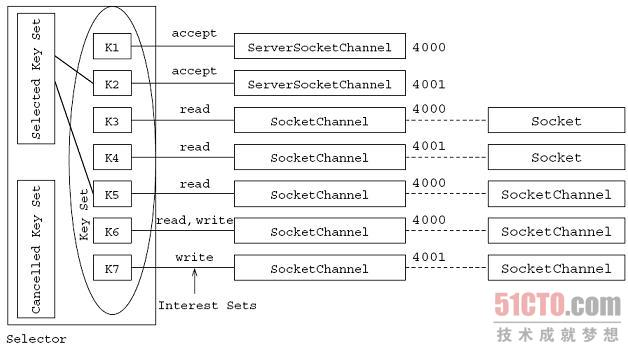
\includegraphics[scale=.6]{img/05.01.jpg}
			\caption{Selector与其关联的键集}
			\label{fig:selector.and.its.key.set}
		\end{figure}

		Selected Key Set: 选择键集;Cancelled Key Set:注销键集;Key Set:键集;Interest Sets:兴趣操作集 

	\subsection{选取和识别准备就绪的信道}

		在信道上注册了选择器,并由关联的键指定了感兴趣的I/O操作集后,我们就只需要坐下来等待I/O了。这要使用选择器来完成。

		Selector: 等待信道准备就绪

		\lstinputlisting[language=Java,firstline=301,lastline=304]{src/ch05/TCPEchoClientNonblocking.txt}

	select()方法用于从已经注册的信道中返回在感兴趣的I/O操作集上准备就绪的信道总数。(例如,兴趣操作集中包含\verb|OP_READ|的信道有数据可读,或包含\verb|OP_ACCEPT|的信道有连接请求待接受。)以上三个select方法的惟一区别在于它们的阻塞行为。无参数的select方法会阻塞等待,直到至少有一个注册信道中有感兴趣的操作准备就绪,或有别的线程调用了该选择器的wakeup()方法(这种情况下select方法将返回0)。以超时时长作为参数的select方法也会阻塞等待,直到至少有一个信道准备就绪,或等待时间超过了指定的毫秒数(正数),或者有另一个线程调用其wakeup()方法。selectNow()方法是一个非阻塞版本:它总是立即返回,如果没有信道准备就绪,则返回0。wakeup()方法可以使当前阻塞(也就是说在另一个线程中阻塞)的任何一种select方法立即返回;如果当前没有select方法阻塞,下一次调用这三种方法的任何一个都将立即返回。

	选择之后,我们需要知道哪些信道准备好了特定的I/O操作。每个选择器都维护了一个已选键集(selected-key set),与这些键关联的信道都有即将发生的特定I/O操作。通过调用selectedKeys()方法可以访问已选键集,该方法返回一组SelectionKey。我们可以在这组键上进行迭代,分别处理等待在每个键关联的信道上的I/O操作。

		\lstinputlisting[language=Java,firstline=307,lastline=312]{src/ch05/TCPEchoClientNonblocking.txt}

		图5.1中的选择器的已选键集中有两个键:K2和K5。

		Selector: 获取键集

		\lstinputlisting[language=Java,firstline=315,lastline=316]{src/ch05/TCPEchoClientNonblocking.txt}

		以上方法返回选择器的不同键集。keys()方法返回当前已注册的所有键。返回的键集是不可修改的:任何对其进行直接修改的尝试(如,调用其remove()方法)都将抛出UnsupportedOperationException异常。selectedKeys()方法用于返回上次调用select()方法时,被"选中"的已准备好进行I/O操作的键。重要提示:selectedKeys()方法返回的键集是可修改的,实际上在两次调用select()方法之间,都必须"手工"将其清空。换句话说,select方法只会在已有的所选键集上添加键,它们不会创建新的键集。

		所选键集指示了哪些信道当前可以进行I/O操作。对于选中的每个信道,我们需要知道它们各自准备好的特定I/O操作。除了兴趣操作集外,每个键还维护了一个即将进行的I/O操作集,称为就绪操作集(ready set)。

		SelectionKey: 查找就绪的I/O操作

		\lstinputlisting[language=Java,firstline=319,lastline=324]{src/ch05/TCPEchoClientNonblocking.txt}

		对于给定的键,可以使用readyOps()方法或其他指示方法来确定兴趣集中的哪些I/O操作可以执行。readyOps()方法以位图的形式返回所有准备就绪的操作集。其他方法用于分别检查各种操作是否可用。

		例如,查看键关联的信道上是否有正在等待的读操作,可以使用以下代码:

		\lstinputlisting[language=Java,firstline=328,lastline=328]{src/ch05/TCPEchoClientNonblocking.txt}

		或

		\lstinputlisting[language=Java,firstline=329,lastline=329]{src/ch05/TCPEchoClientNonblocking.txt}

		选择器的已选键集中的键,以及每个键中准备就绪的操作,都是由select()方法来确定的。随着时间的推进,这些信息可能会过时。其他线程可能会处理准备就绪的I/O操作。同时,键也不是永远存在的。当其关联的信道或选择器关闭时,键也将失效。通过调用其cancel()方法可以显示地将键设置为无效。调用其isValid()方法可以检测一个键的有效性。无效的键将添加到选择器的注销键集中,并在下次调用任一种形式的select()方法或close()方法时从键集中移除。(当然,从键集中移除键意味着与它关联的信道也不再受监听。)

	\subsection{信道附件附件}


		当一个信道准备好进行I/O操作时,通常还需要额外的信息来处理请求。例如,在前面的回显协议中,当客户端信道准备好写操作时,就需要有数据可写。当然,我们所需要的可写数据是由之前同一信道上的读操作收集的,但是在其可写之前,这些数据存放在什么地方呢?另一个例子是第3章中的成帧过程。如果一个消息一次传来了多个字节,我们需要保存已接收的部分消息,直到完整个消息接收完成。这两种情况都需要维护每个信道的状态信息。然而,我们非常幸运!SelectionKey通过使用附件使保存每个信道的状态变得容易。

		SelectionKey: 查找准备就绪的I/O操作

		\lstinputlisting[language=Java,firstline=331,lastline=332]{src/ch05/TCPEchoClientNonblocking.txt}

		每个键可以有一个附件,数据类型只能是Object类。附件可以在信道第一次调用register()方法时与之关联,或者后来再使用attach()方法直接添加到键上。通过SelectionKey的attachment()方法可以访问键的附件。 

	\subsection{Selector小结}

		总的来说,使用Selector的步骤如下:

		I.创建一个Selector实例。

		II.将其注册到各种信道,指定每个信道上感兴趣的I/O操作。

		III.重复执行:

		1.调用一种select方法。

		2.获取选取的键列表。

		3.对于已选键集中的每个键,

		a.获取信道,并从键中获取附件(如果合适的话)

		b.确定准备就绪的操作并执行。如果是accept操作,将接受的信道设置为非阻塞模式,并将其与选择器注册。

		c.如果需要,修改键的兴趣操作集

		d.从已选键集中移除键

		如果选择器告诉了你什么时候I/O操作准备就绪,你还需要非阻塞I/O吗?答案是肯定的。信道在已选键集中的键并不能确保非阻塞I/O,因为调用了select()方法后,键集信息可能会过时。另外,阻塞式写操作会阻塞等待直到写完所有的字节,而就绪集中的\verb|OP_WRITE|仅表示至少有一个字节可写。实际上,只有非阻塞模式的信道才能与选择器进行注册:如果信道在阻塞模式,SelectableChannel类的register()方法将抛出IllegalBlockingModeException异常。

\section{数据报(UDP)信道}

	Java的NIO包通过DatagramChannel类实现了数据报(UDP)信道。与我们之前看到的其他形式的SelectableChannel一样,DatagramChannel在DatagramSocket上添加了选择和非阻塞行为,以及基于缓冲区的I/O操作能力。

	DatagramChannel: 创建,连接和关闭

	\lstinputlisting[language=Java,firstline=336,lastline=338]{src/ch05/TCPEchoClientNonblocking.txt}

	需要调用DatagramChannel的open()工厂方法来创建一个DatagramChannel实例,该实例是未绑定的。DatagramChannel只是对基本DatagramSocket的一个包装器(wrapper)。使用其socket()方法可以直接访问内部的DatagramSocket实例。这就允许通过调用基本的DatagramSocket方法进行绑定、设置套接字选项等操作。用完DatagramChannel后,要调用它的close()方法将其关闭。

	只要创建了一个DatagramChannel实例,就可以非常直接地发送和接收数据。

	DatagramChannel: 发送和接收

	\lstinputlisting[language=Java,firstline=341,lastline=342]{src/ch05/TCPEchoClientNonblocking.txt}

	send()方法用于创建一个包含了给定ByteBuffer中的数据的数据报文,并将其发送到目的地址指定的SocketAddress上。receive()方法用于将接收到的数据报文存入指定缓冲区并返回发送者的地址。重要提示:如果缓冲区的剩余空间小于数据报文中的数据大小,多余的数据将毫无提示地丢弃。

	以下代码段用于创建一个DatagramChannel实例,并将UTF-16编码的字符串"Hello"发送到运行在同一主机的5000端口上的UDP服务器上。

	\lstinputlisting[language=Java,firstline=344,lastline=346]{src/ch05/TCPEchoClientNonblocking.txt}

	以下代码段用于创建一个DatagramChannel实例,将底层的套接字绑定到5000端口,接收最长为20字节的数据报文,并将字节转换成使用UTF-16编码的字符串。

	\lstinputlisting[language=Java,firstline=348,lastline=354]{src/ch05/TCPEchoClientNonblocking.txt}

	在上面的send()实例中,调用send()方法时并没有显式地绑定本地端口,因此将随机选择一个可用端口。相应的receive()方法用于返回一个SocketAddress,其中包含了端口号。

	如果总是向同一个远程终端发送或接收数据,我们可以选择调用connect()方法,并使用 SocketAddress指定远程终端的地址。

	DatagramChannel: 连接DatagramChannel

	\lstinputlisting[language=Java,firstline=358,lastline=366]{src/ch05/TCPEchoClientNonblocking.txt}

	这些方法限制我们只能通过指定的地址发送和接收数据。为什么要这样做呢?原因之一是调用connect()方法后,可以使用read()和write()方法来代替receive()和send()方法,并且不需要处理远程地址。read()和write()方法分别用于接收和发送一个数据报文。分散式读操作以一个ByteBuffer数组为参数,只接收一个数据报文,并按顺序将其填入缓冲区中。聚集式写操作将缓冲区数组中的所有字节连接起来创建一个要传输的数据报文。重要提示:现在能够发送的最大数据报文可以包含65507个字节,试图发送更多的数据将被无提示地截断。

	使用connect()方法的另一个好处是,已建立连接的数据报文信道可能只接收从指定终端发送来的数据,因此我们不需要测试接收端的有效性。注意,DatagramChannel的connect()方法只起到限制发送和接收终端的作用,连接时并没有数据包在SocketChannel上进行交换,而且也不需要像SocketChannel那样等待或测试连接是否完成。(见第6章)

	到目前为止DatagramChannel看起来与DatagramSocket非常相似。数据报文信道和套接字的主要区别是,信道可以进行非阻塞I/O操作和使用选择器。DatagramChannel中选择器的创建,信道的注册、选择等,与SocketChannel几乎一模一样。有一个区别是DatagramChannel不能注册连接I/O操作,不过也不需要这样做,因为DatagramChannel的connect()方法永远不会阻塞。

	DatagramChannel: 设置阻塞行为和使用选择器

	\lstinputlisting[language=Java,firstline=371,lastline=377]{src/ch05/TCPEchoClientNonblocking.txt}

	这些方法的功能与SocketChannel和ServerSocketChannel中的相应方法一样。

	下面使用DatagramChannel对第4章中的DatagramSocket UDP回显服务器进行重写。服务器侦听指定的端口,并将接收到的数据报文简单地回发给客户端。重写后的服务器与原来版本的主要区别是它不会在send()和receive()方法上阻塞等待。

	\lstinputlisting[language=Java,firstline=1]{src/ch05/UDPEchoServerSelector.java}

		\chapter{深入剖析} 

	如果不理解套接字的具体实现所关联的数据结构和底层协议的工作细节,就很难抓住网络编程的精妙之处,对于TCP套接字(即Socket的实例)来说更是如此。本章就对创建和使用Socket或ServerSocket实例时的底层细节进行了介绍。(本章开始的讨论以及第6.5节同样适用于DatagramSocket和MulticastSocket。而且,由于每个SocketChannel都有一个底层的Socket(其他类型的信道也类似),我们讨论的内容也同样适用于它们。然而,本章大部分内容都针对的是TCP套接字,即,Socket和ServerSocket。)请注意,这些内容仅仅涵盖了一些普通的事件序列,略去了很多细节。尽管如此,我们相信即使是这种基础的理解也是有用的。如果希望了解更详尽内容,可以参考TCP规范[ ],或关于该主题的其他更全面的著作。

	图6.1是一个Socket实例所关联的一些信息的简化视图。JVM和/或其运行的平台(即,主机操作系统中的"套接字层")为这些类的支持提供了底层实现。Java对象上的操作则转换成了在这种底层抽象上的操作。在本章中,"Socket"指的是图6.1中的类之一,而"套接字(socket)"指的是的底层抽象,这种抽象由操作系统提供或由JVM自己实现(例如在嵌入式系统中)。有重要一点需要注意,即运行在统一主机上的其他程序可能也会通过底层套接字抽象来使用网络,因此会与Java Socket实例竞争系统资源,如端口等。

	\clearpage

	\begin{figure}[htbp]%位置选项
		\centering
		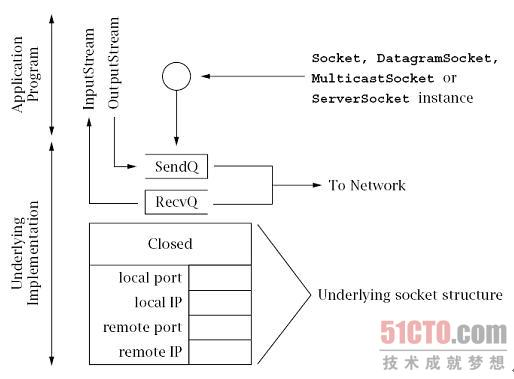
\includegraphics[scale=.6]{img/06.01.jpg}
		\caption{套接字关联的数据结构}
		\label{fig:data.struct.of.socket}
	\end{figure}

	Application Program:应用程序;Underlying Implementation:底层实现;To Network:到网络;Underlying socket structure:底层套接字结构;Socket, DatagramSocket, MulticastSocket or ServerSocket instance:Socket,DatagramSocket,MulticastSocket或ServerSocket实例;

	在此,"套接字结构"是指底层实现(包括JVM和TCP/IP,但通常是后者)的数据结构集,这些数据结构包含了特定Socket实例所关联的信息。例如,套接字结构除其他信息外还包含

	该套接字所关联的本地和远程互联网地址和端口号。本地互联网地址(图中标记为"Local IP")是赋值给本地主机的;本地端口号在Socket实例创建是设置。远程地址和端口号标识了与本地套接字连接的远程套接字(如果有连接的话)。不久,我们将对这些值确定的时间和方式作进一步介绍(第6.5节中有一个简明的概要)。

	一个FIFO(先进先出,First In First Out)队列用于存放接收到的等待分配的数据,以及一个用于存放等待传输的数据的队列。

	对于TCP套接字,还包含了与打开和关闭TCP握手相关的额外协议状态信息。图6.1中,状态是"关闭";所有套接字的起始状态都是关闭的。

	一些多用途操作系统为用户提供了获取底层数据结构"快照"的工具,netstat是其中之一,它在Unix(Linux)和Windows平台上都可用。只要给定适当的选项,netstat就能显示和图6.1中的那些信息:SendQ和RecvQ中的字节数,本地和远程IP地址和端口号,以及连接状态等。netstat的命令行选项有多种,但它的输出看起来是这样的:

	\lstinputlisting[language=Bash,firstline=1,lastline=10]{src/ch06/stp.txt}

	前四行和最后一行描述了正在侦听连接的服务器套接字。(最后一行是一个绑定到IPv6地址的侦听套接字。)第五行代表了到一个Web服务器(80端口)的连接,该服务器已经单方面关闭(见第6.4.2节)。倒数第二两行是现有的TCP连接。如果系统支持的话,你可能想要尝试一下netstat,来测试下文描述的场景的连接状态。然而要知道,这些图中描述的状态转换过程转瞬即逝,可能很难通过netstat提供的"快照"功能将其捕获。

	了解这些数据结构,以及底层协议如何对其进行影响是非常有用的,因为它们控制了各种Socket对象行为的各个方面。例如,由于TCP提供了一种可信赖的字节流服务,任何写入Socket的OutputStream的数据复本都必须保留,直到其在连接的另一端被成功接收。向输出流写数据并不意味着数据实际上已经被发送--它们只是被复制到了本地缓冲区。就算在Socket的OutputStream上进行flush()操作,也不能保证数据能够立即发送到信道。此外,字节流服务的自身属性决定了其无法保留输入流中消息的边界信息。如在第3.3节见到的,这使一些协议的接收和解析过程变得复杂。另一方面,对于DatagramSocket,数据包并没有为重传而进行缓存,任何时候调用send()方法返回后,数据就已经发送给了执行传输任务的网络子系统。如果网络子系统由于某种原因无法处理这些消息,该数据包将毫无提示地被丢弃(不过这种情况很少发生)。

	后面3节对使用TCP字节流服务发送和接收数据的一些微妙之处进行了介绍。然后,第6.4节专注于TCP协议连接的建立和终止。最后,第6.5节讨论了匹配传入的数据包到套接字的过程和绑定端口号的一些规则。

\section{缓冲和TCP}

	作为程序员,在使用TCP套接字时需要记住的最重要一点是:

	不能假设在连接的一端将数据写入输出流和在另一端从输入流读出数据之间有任何一致性。

	尤其是在发送端由单个输出流的write()方法传输的数据,可能会通过另一端的多个输入流的read()方法来获取;而一个read()方法可能会返回多个write()方法传输的数据。

	为了展示这种情况,考虑如下程序:

	\lstinputlisting[language=Java,firstline=15,lastline=28]{src/ch06/stp.txt}

	其中,圆点代表了设置缓冲区数据的代码,但不包含对out.write()方法的调用。在本节的讨论中,"in"代表接收端Socket的InputStream,"out"代表发送端Socket的OutputStream。

	这个TCP连接向接收端传输8000字节。在连接的接收端,这8000字节的分组方式取决于连接两端out.write()方法和in.read()方法的调用时间差,以及提供给in.read()方法的缓冲区大小。

	我们可以认为TCP连接上发送的所有字节序列在某一瞬间被分成了三个FIFO队列:

	1. SendQ:在发送端底层实现中缓存的字节,这些字节已经写入输出流,但还没在接收端主机上成功接收。

	2. RecvQ:在接收端底层实现中缓存的字节,等待分配到接收程序--即从输入流中读取。

	3. Delivered:接收者从输入流已经读取到的字节。

	调用out.write()方法将向SendQ追加字节。TCP协议负责将字节按顺序从SendQ移动到RecvQ。有重要的一点需要明确,这个转移过程无法由用户程序控制或直接观察到,并且在块中(chunks)发生,这些块的大小在一定程度上独立于传递给write()方法的缓冲区大小。

	接收程序从Socket的InputStream读取数据时,字节就从RecvQ移动到Delivered中,而转移的块的大小依赖于RecvQ中的数据量和传递给read()方法缓冲区大小。

	图6.2展示了上例中三次调用out.write()方法后,另一端调用in.read()方法前,以上3个队列的可能状态。不同的阴影效果分别代表了上文中三次调用write()方法传输的不同数据。

	图6.2描述的发送端主机的netstat输出瞬时状态中,会包含类似于以下一行的内容:

	\lstinputlisting[language=Bash,firstline=31,lastline=33]{src/ch06/stp.txt}

	在接收端主机,netstat会显示:

	\lstinputlisting[language=Bash,firstline=35,lastline=37]{src/ch06/stp.txt}

	现在假设接收者调用read()方法时使用的缓冲区数组大小为2000字节,read()调用则将把等待分配队列(RecvQ)中的1500字节全部移动到数组中,返回值为1500。注意,这些数据包括了第一次和第二次调用write()方法时传输的字节。再过一段时间,当TCP连接传完更多数据后,这三部分的状态可能如图6.3所示。

	如果接收者现在调用read()方法时使用4000字节的缓冲区数组,将有很多字节从等待分配队列(RecvQ)转移到已分配队列(Delivered)中。这包括第二次调用write()方法时剩下的1500字节加上第三次调用write()的前2500字节。此时队列的状态如图6.4所示。

	\clearpage

	\begin{figure}[htbp]%位置选项
		\centering
		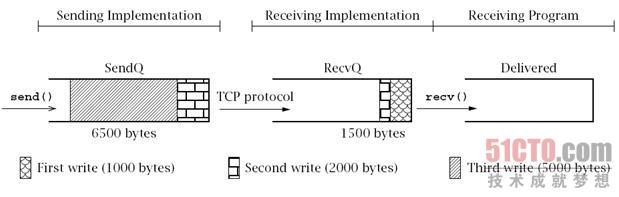
\includegraphics[scale=.6]{img/06.02.jpg}
		\caption{三次调用write()方法后三个队列的状态}
		\label{fig:tree.time.call.write.get.tree.query}
	\end{figure}

	Sending Implementation:发送实现,Receiving Implementation:接收实现,6500 bytes:6500字节,1500 bytes:1500字节,Receiving Program:接收程序,First write(1000 bytes):第一次写操作(1000字节),Second write(2000 bytes):第二次写操作(2000字节),Third write(5000 bytes):第三次写操作(5000字节),TCP protocol:TCP协议

	\clearpage

	\begin{figure}[htbp]%位置选项
		\centering
		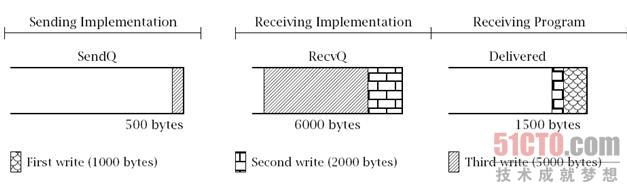
\includegraphics[scale=.6]{img/06.03.jpg}
		\caption{第一次调用read()方法}
		\label{fig:first.time.call.read.func}
	\end{figure}

	Sending Implementation:发送实现,Receiving Implementation:接收实现,500 bytes:500字节,6000 bytes:6000字节,1500 bytes:1500字节,First write(1000 bytes):第一次写操作(1000字节),Second write(2000 bytes):第二次写操作(2000字节),Third write(5000 bytes):第三次写操作(5000字节)

	\clearpage

	\begin{figure}[htbp]%位置选项
		\centering
		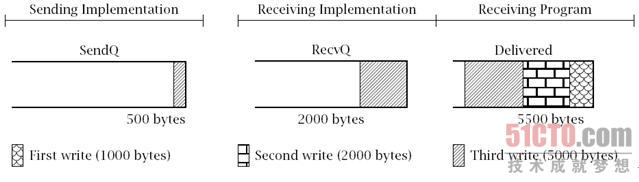
\includegraphics[scale=.6]{img/06.04.jpg}
		\caption{另一次调用read()方法}
		\label{fig:another.call.read.func}
	\end{figure}

	Sending Implementation:发送实现,Receiving Implementation:接收实现,500 bytes:500字节,2000 bytes:2000字节,5500 bytes:5500字节,First write(1000 bytes):第一次写操作(1000字节),Second write(2000 bytes):第二次写操作(2000字节),Third write(5000 bytes):第三次写操作(5000字节)

	下次调用read()方法返回的字节数,取决于缓冲区数组的大小,以及发送方套接字/TCP实现通过网络向接收方实现传输数据的时机。数据从SendQ到RecvQ缓冲区的移动过程对应用程序协议的设计有重要的指导性。我们已经遇到过需要对使用带内(in-band)分隔符成帧(见第3.3节),并通过Socket来接收的消息进行解析的情况。在下面的章节中,我们将考虑另外两个更加微妙的情况。

\section{死锁风险}

	应用程序协议必须设计得非常小心,以避免发生死锁--这种情况下,每个对等端都在阻塞等待其他端完成一些工作。例如,如果在连接建立后,客户端和服务器端都立即尝试接收数据,显然将导致死锁。死锁还可能发生在其他非即时的情况下。

	SendQ和RecvQ缓冲区的容量在具体实现时会受一定的限制。虽然它们使用的实际内存大小会动态地增长和收缩,还是需要有一个硬性的限制,以防止行为异常的程序所控制的单独一个TCP连接将系统的内存全部耗尽。由于这些缓冲区的容量有限,它们可能被填满,事实也的确如此。如果与TCP的流量控制(flow control)机制结合使用,则可能导致另一种形式的死锁。

	一旦RecvQ已满,TCP流控制机制就会产生作用。它将阻止传输发送端主机的SendQ中的任何数据,直到接收者调用输入流的read()方法后腾出了空间。(使用流控制机制的目的是为了保证发送者不会传输太多数据,而超出了接收系统的处理能力。)发送程序可以持续地写出数据,直到SendQ队列被填满,然而,如果在SendQ队列已满时调用out.write()方法,则将阻塞等待,直到有新的空间为止,也就是说直到一些字节传输到了接收到套接字的RecvQ队列中。如果此时RecvQ队列也已经被填满,所有操作都将停止,直到接收程序调用in.read()方法将一些字节传输到了Delivered队列中。

	假设SendQ队列和RecvQ队列的大小分别为SQS和RQS。将一个大小为n的字节数组传递给write()方法调用,其中n > SQS,直到有至少n- SQS字节传递到接收端主机的RecvQ队列后,该方法才会返回。如果n的大小超过了(SQS + RQS),write()方法则将在接收程序从输入流读取了至少n? (SQS + RQS)字节后才会返回。如果接收程序没有调用read()方法,大数据量的send()调用则无法成功。特别是当连接的两端同时分别调用它们输出流的write()方法,而它们的缓冲区大小又大于SQS + RQS时,将发生死锁:两个write操作都不能完成,两个程序都将永远保持阻塞状态。

	下面考虑一个具体的例子,即主机A上的程序和主机B上的程序之间的一个连接。假设A和B上的SQS和RQS都是500字节,图6.5展示了两个程序试图同时发送1500字节时的情况。主机A上的程序中的前500字节已经传输到了另一端,另外500字节已经复制到了主机A的SendQ队列中,余下的500字节则无法发送(因此out.write()方法将无法返回)直到主机B上的RecvQ队列有空间空出来。然而不幸的是主机B上的程序也遇到了同样的情况。因此两个程序的write()方法调用都永远无法完成。

	\clearpage

	\begin{figure}[htbp]%位置选项
		\centering
		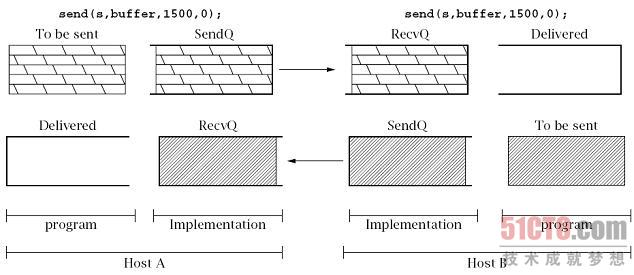
\includegraphics[scale=.6]{img/06.05.jpg}
		\caption{由于连接两端同时调用输出流的write()方法而导致了死锁}
		\label{fig:dead.lock.by.call.both.side}
	\end{figure}

	program:程序,Implementation:具体实现, To be sent:即将发送

	这个故事的寓意:要仔细设计协议,以避免在两个方向上传输大量数据时产生死锁。

	这种情况真的会发生吗?让我们回顾一下第4.5节中的压缩协议示例。尝试运行该压缩客户端并传递给它一个大文件,该文件压缩后仍然很大。在此,"大"的精确定义取决于你的系统,不过压缩后依然超过2MB的文件应该就可以了。每次read/write操作,压缩客户端都向控制台打印一个"R"或"W"。如果该文件的未压缩版本和压缩版本都足够大,你的客户端将在打印出一堆W后停止,并且不会打印任何R,程序也不过终止。

	为什么会发生这种情况呢?程序CompressClient.java在尝试从压缩流读取数据前,先要将所有未压缩的数据发送到压缩服务器。而另一方面,服务器只是简单地读取未压缩字节序列,并将压缩后的序列返回给客户端。(服务器在写回压缩数据前,其读取的字节数取决于所使用的压缩算法。)考虑这种情况:客户端和服务器端的SendQ队列和RecvQ队列中都有500字节的数据,而客户端发送了一个大小为10000字节(未压缩)的文件。同时假设对于这个文件,服务器读取1000字节并返回500字节,即压缩比为2:1。当客户端发送了2000字节后,服务器端将最终全部读取这些字节,并发回1000字节,此时客户端的RecvQ队列和服务器端的SendQ队列都将被填满。当客户端又发送了1000字节并且被服务器端全部读取后,服务器端后续的任何write操作尝试都将阻塞。当客户端又发送了另外1000字节后,客户端的SendQ队列和服务器端的RecvQ队列都将填满。后续的客户端write操作将阻塞,从而形成死锁。

	\lstinputlisting[language=Java,firstline=1]{src/ch06/CompressClient.java}

	如何解决这个问题?方案之一是在不同的线程中执行客户端的write循环和read循环。一个线程从文件中反复读取未压缩的字节并将其发送给服务器,直到到底文件的结尾,然后调用该套接字的shutdownOutput()方法。另一个线程从连接到服务器的输入流中反复读取压缩后的字节,并将其写入输出文件,直到到达了输入流的结尾(即服务器关闭了套接字)。如果一个线程阻塞了,另一个线程仍然可以独立执行。要实现这个功能,我们可以对客户端代码进行简单的修改,像下面这样将CompressClient.java中的SendBytes()方法调用放到一个线程中:

	\lstinputlisting[language=Java,firstline=41,lastline=48]{src/ch06/stp.txt}

	CompressClientNoDeadlock.java的完整版本请参见本书的网站。

	\lstinputlisting[language=Java,firstline=1]{src/ch06/CompressClientNoDeadlock.java}

	当然,解决这个问题也可以不使用多线程,而是使用第5章介绍的非阻塞Channel和Selector。

\section{性能相关}

	在TCP实现中,将用户数据复制到SendQ队列中不仅是因为可能重传数据,这还与性能有关。尤其是SendQ和RecvQ缓冲队列的大小,会对TCP连接的数据吞吐量产生影响。吞吐量是指用户数据字节从发送端发送到接收程序的频率。在要传输大量数据的程序中,我们希望能够最大化这个频率。在没有网络容量或其他限制的情况下,越大的缓冲区通常能够实现越高的吞吐量。

	这种情况发生的原因,与底层实现中将数据从缓冲区中存取时的系统耗费有关。如果要传输n字节的数据,使用大小为n的缓冲区调用一次write()方法,通常要比使用大小为1字节的缓冲区调用n次write()方法效率要高很多。[ ] 然而,如果调用write()方法时使用了比SQS(SendQ队列的大小)大很多的缓冲区,系统还需要将数据从用户地址转换为大小为SQS的块(chunks)。也就是说,套接字底层实现先将SendQ队列缓冲区填满,等待TCP协议将数据转移出去,再重新填满SendQ队列缓冲区,再等待数据转移,反复进行。套接字底层实现每次都要等待数据从SendQ队列中移出,这就以系统耗费的形式(系统需要进行上下文切换)浪费了一些时间。这种系统耗费与重新调用一次write()方法的情况相似。因此,调用write()方法时的实际有效缓冲区大小要受SQS的限制。从InputStream读取数据也是一样的道理:即使提供给read()方法的缓冲区很大,数据还是会被复制成RQS大小的块,在块之间又会产生新的系统耗费。

	如果程序的数据吞吐量是一个重要的性能参数,你可能希望通过Socket的setSendBufferSize()和setReceiveBufferSize()方法来改变发送和接收缓冲区的大小。虽然每个缓冲区都有系统指定的最大容量,但是在现代系统上缓冲区的容量通常要比系统的默认大小要大很多。要记住一点,只有当程序要一次发送比缓冲区容量大很多的数据时才需要考虑这些情况。同时还有注意,如果处理了一些从Socket的基本输入流继承而来的更高层次的流(例如,使用它来创建一个FilterOutputStream实例或PrintWriter实例),这些因素产生的效果就会略有不同,因为更高层次的流可能会执行它们字节的内部缓存或增加额外的系统开销。


	\subsection{TCP套接字的生存周期}

		新的Socket实例创建后(无论是通过公有的构造函数,或是通过调用ServerSocket类的accept()方法)立即就能用于发送和接收数据。也就是说,当Socket实例返回时,它已经连接到了一个远程终端,并通过协议的底层实现完成了TCP消息或握手信息的交换。

		下面,让我们进一步详细考虑底层的数据结构如何到达已连接或"已建立(Established)"状态。后面你将看到,这些细节会对可靠性的定义和创建一个绑定到特定端口的Socket或ServerSocket的能力产生影响。

		\subsection{连接}

		Socket构造函数的调用与客户端连接建立时所关联的协议事件之间的关系如图6.6所示。在本节所有的示意图中,大箭头都表示导致底层套接字数据结构发生状态改变的外部事件。在应用程序中发生的事件(即方法调用和返回)显示在图个上部;如消息到达等事件显示在图的下部。所有图的时间顺序都是从左到右的;客户端的互联网地址表示为A.B.C.D,服务器端的互联网地址表示为W.X.Y.Z; 服务器的端口号是Q。(我们描述的是IPv4地址,不过这里介绍的内容都适用于IPv4和IPv6。)

		当客户端以服务器端的互联网地址W.X.Y.Z和端口号Q作为参数,调用Socket的构造函数时,底层实现将创建一个套接字实例,该实例的初始状态是关闭状态(Closed)。如果在调用构造函数时客户端没有指定本地地址或端口号,底层实现将选择一个没有被其他TCP套接字使用的本地端口号(P)。同时还要指定本地的互联网地址,如果没有显式地指定,则将向服务器发送数据报文的网络接口地址作为本地地址。底层实现将本地和远程地址和端口复制到底层套接字的数据结构,并初始化TCP连接建立时的握手消息。

		\clearpage

		\begin{figure}[htbp]%位置选项
			\centering
			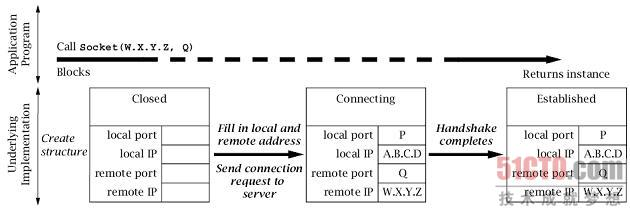
\includegraphics[scale=.6]{img/06.06.jpg}
			\caption{客户端连接建立}
			\label{fig:client.create.connection}
		\end{figure}

		Application Program:应用程序,Underlying Implementation:底层实现,Call Socket(W.X.Y.Z,Q):调用Socket(W.X.Y.Z,Q),Blocks:阻塞等待,Create structure:创建数据结构,local port:本地端口,local IP:本地IP地址,remote port:远程端口号,remote IP:远程IP地址,Fill in local and remote address:填入本地和远程地址,Send connection request to server:向服务器发送连接请求,Handshake completes:握手消息完成,Returns instance:返回实例,Connecting:正在连接,Established:连接建立完成

		TCP的开放握手也称为3次握手(3-way handshake),因为这通常包括3条消息:一条从客户端到服务器端的连接请求,一条从服务器端到客户端的确认消息,以及另一条从客户端到服务器端的确认消息。客户端一收到服务器端发来的确认消息,就立即认为连接已经成功建立。通常情况这个过程发生得很快。然而,互联网是一种尽力而为(best-effort)的网络,客户端的起始消息或服务器端的回复消息都可能在传输过程中丢失。出于这个原因,TCP协议实现将以递增的时间间隔重复发送几次握手消息。如果TCP客户端在一段时间后还没有收到服务器的回复消息,则发生超时并放弃连接。这种情况下,构造函数将抛出IOException异常。连接的超时通常比较长,因此要经过几分种的时间Socket的构造函数才会失败。

		在初始的握手消息发送之后,并在接收到服务器端的回复消息之前(即图6.6的中间部分),客户端主机上netstat的输出将类似于以下内容:

		\lstinputlisting[language=Java,firstline=51,lastline=53]{src/ch06/stp.txt}

		其中,"\verb|SYN_SENT|"是在第一条和第二条握手消息之间,客户端状态的专业名称。

		如果服务器并没有接收连接(比如,目标地址的给定端口上没有关联任何程序),服务器端的TCP将发送一条拒绝消息而不是确认消息,并且构造函数几乎立即会抛出一个IOException异常。否则,在客户端收到了服务器端的肯定回复后,其netstat的输出将类似于以下内容:

		\lstinputlisting[language=Java,firstline=56,lastline=58]{src/ch06/stp.txt}

		服务器端的事件序列则有所不同,我们在图6.7,6.8和6.9中对其进行描述。服务器首先创建一个ServerSocket实例,并将其与已知端口相关联(在此为Q)。套接字实现为新的ServerSocket实例创建了一个底层数据结构,并将Q赋给本地端口,将特定的通配符地址(图中的"*")赋给本地IP地址。(服务器也可能会在构造函数中指定一个本地IP地址,但是通常不这样做。对于服务器主机有多个IP地址的情况,不指定本地地址使套接能够接受发送到该服务器主机任何地址的连接请求。)套接字的状态设置为"LISTENING",指示该套接已经准备好接受传入该端口的连接请求。图6.7描述了这个过程。服务器端netstat的输出中会包含类似于如下一行的内容:

		\lstinputlisting[language=Java,firstline=61,lastline=63]{src/ch06/stp.txt}

		\clearpage

		\begin{figure}[htbp]%位置选项
			\centering
			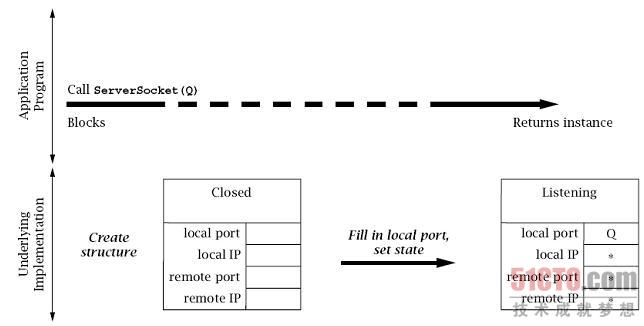
\includegraphics[scale=.6]{img/06.07.jpg}
			\caption{服务器端套接字设置}
			\label{fig:server.create.socket}
		\end{figure}

		Application Program:应用程序;Underlying Implementation:底层实现;Call ServerSocket(Q):调用ServerSocket(Q);Blocks:阻塞等待;Returns instance:返回实例;Create structure:创建数据结构;Closed:关闭;Listening:侦听;local port:本地端口;local IP:本地IP地址;remote port:远程端口号;remote IP:远程IP地址;Fill in local port,set stat:填入本地端口号,设置状态;

		现在服务器可以调用ServerSocket的accept()方法,该方法将阻塞等待,直到与某个客户端完成了开放握手信息交换,并成功建立了新的连接。因此我们关注于(见图6.8)当客户端连接请求到来时,TCP实现中发生的事件。注意,该图中描述的内容全都隐蔽地发生在TCP底层实现中。

		当客户端的连接请求到来时,将为该连接创建一个新的套接字数据结构。新套接字的地址根据到来的分组报文设置:分组报文的目标互联网地址和端口号(分别为W.X.Y.Z和Q)成为该套接字的本地互联网地址和端口号;而分组报文的源地址和端口号(分别为A.B.C.D和P)则成为该套接字的远程互联网地址和端口号。注意,新套接字的本地端口号总是与ServerSocket的端口号一致。新套接字的状态设置为指示"正在连接(Connecting)"(在服务器方,专业术语称其为\verb|SYN_RCVD|),并将其添加到ServerSocket套接字数据结构所关联的一个未完全连接的套接字列表中。注意,ServerSocket自己并不改变状态,其地址信息也不会有任何改变。此时,netstat的输出内容应该包括原始的侦听套接字和新创建的套接字:

		\lstinputlisting[language=Java,firstline=65,lastline=68]{src/ch06/stp.txt}

		除了要创建一个新的底层套接字数据结构外,服务器方的TCP实现还要向客户端发回一个TCP握手确认消息。

		\clearpage

		\begin{figure}[htbp]%位置选项
			\centering
			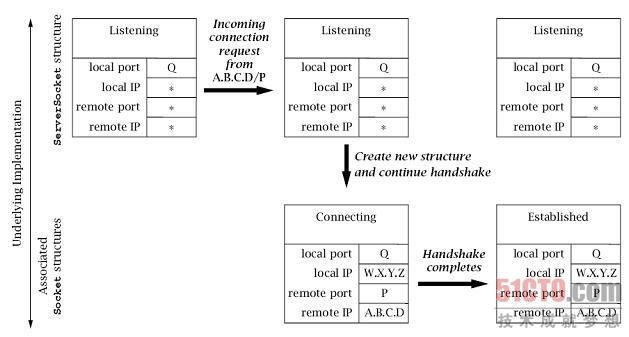
\includegraphics[scale=.6]{img/06.08.jpg}
			\caption{处理传入的连接请求}
			\label{fig:deal.income.connect.req}
		\end{figure}

		Underlying Implementation:底层实现;Associated Socket structures:关联的Socket数据结构;ServerSocket structure:ServerSocket数据结构;local port:本地端口;local IP:本地IP地址;remote port:远程端口号;remote IP:远程IP地址;Listening:侦听;Connecting:正在连接;Established:连接建立;Incoming connection request from A.B.C.D/P:从A.B.C.D/P传来的连接请求;Create new structure and continue handshake:创建新的数据结构并继续握手;Handshake completes:握手完成。

		然而,在接收到客户端发来的3次握手的第3条消息之前,服务器端TCP并不会认为握手消息已经完成。第3条握手消息到来后,新数据结构的状态则设置为"ESTABLISHED",并将其移动到ServerSocket数据结构关联的另一个套接字数据结构列表中,该列表代表了能够通过ServerSocket的accept()方法进行接收的已成功建立连接。(如果第3条握手消息接收失败,最终会将"Connecting"状态的数据结构删除。)此时netstat的输出将包含:

		\lstinputlisting[language=Java,firstline=71,lastline=74]{src/ch06/stp.txt}

		现在,我们来考虑(见图6.9)服务器程序调用了ServerSocket的accept()方法后发生的事情。只要其关联的套接字数据结构列表中有新的连接到来,该方法调用就立即停止阻塞。(注意,在调用accept()方法时,这个列表可能已经是非空状态。)此时,一个新的连接数据结构将从列表中移除,并为其创建一个Socket实例,作为accept()方法的返回值。

		有非常重要的一点需要注意,在ServerSocket关联的列表中的每个数据结构,都代表了一个与另一端的客户端已经完成建立的TCP连接。实际上,客户端只要接收到了开放握手的第2条消息,就可以立即发送数据--这可能比服务器调用accept()方法为其获取一个Socket实例要早很长时间。

		\clearpage

		\begin{figure}[htbp]%位置选项
			\centering
			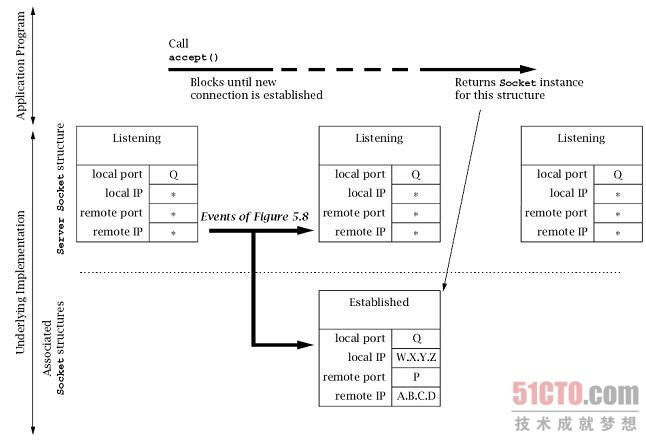
\includegraphics[scale=.6]{img/06.09.jpg}
			\caption{accept()处理}
			\label{fig:accept.process}
		\end{figure}

		Application Program:应用程序;Underlying Implementation:底层实现;Associated Socket structures:关联的Socket数据结构;ServerSocket structure:ServerSocket数据结构;Call accept():调用accept()方法;Blocks until new connection is established:阻塞等待,直到建立了新的连接;Return Socket instance for this structure:为此数据结构返回Socket实例;local port:本地端口;local IP:本地IP地址;remote port:远程端口号;remote IP:远程IP地址;Events of Figure 5.8:图5.8中的事件;Listening:侦听;Established:连接建立。

	\subsection{关闭TCP连接}

		TCP协议有一个优雅的关闭(graceful close)机制,以保证应用程序在关闭连接时不必担心正在传输的数据会丢失。如第4.5节的压缩示例程序所示,这个机制还设计为允许两个方向的数据传输相互独立地终止。关闭机制的工作流程是:应用程序通过调用连接套接字的close()方法或shutdownOutput()方法表明数据已经发送完毕。此刻,底层的TCP实现首先将留存在SendQ队列中的数据传输出去(还要依赖于另一端RecvQ队列的剩余空间),然后向另一端发送一个关闭TCP连接的握手消息。该关闭握手消息可以看作是流终止标志:它告诉接收端TCP不会再有新的数据传入RecvQ队列了。(注意,关闭握手消息本身并没有传递给接收端应用程序,而是通过read()方法返回-1来指示其在字节流中的位置。)正在关闭的TCP将等待其关闭握手消息的确认信息,该确认信息表明在连接上传输的所有数据已经安全地传输到了RecvQ中。只要收到了确认消息,该连接就变成"半关闭(Half closed)"状态。直到连接的另一个方向上收到了对称的握手消息后,连接才完全关闭--也就是说,连接的两端都表明它们再没有数据要发送了。

		TCP连接的关闭事件序列可能以两种方式发生:一种方式是先由一个应用程序调用close()方法(或shutdownOutput()方法),并在另一端调用close()方法之前完成其关闭握手消息;另一种方式是两端同时调用close()方法,它们的关闭握手消息在网络上交叉传输。图6.10展示了以第一种方式关闭连接时,底层实现中的事件序列。关闭握手消息已经发送,套接字数据结构的状态也已经设置为"Closing"(专业术语称为"\verb|FIN_WAIT_1|"),然后close()调用返回。完成这些工作后,将禁止在该Socket上的任何读写操作(会抛出异常)。当收到关闭握手确认消息后,套接字数据结构的状态则改变为"半关闭"(专业术语称为"\verb|FIN_WAIT_2|"),这种状态将一直持续,直到接收到另一端的关闭握手消息。此时,客户端netstat的输出内容将展示连接的状态为:

		\lstinputlisting[language=Java,firstline=77,lastline=79]{src/ch06/stp.txt}

		(在首先发起关闭的主机上,\verb|FIN_WAIT_2|是"半关闭"状态的专业术语。图中由"Closing"指示的状态的专业术语是\verb|FIN_WAIT_1|,不过该状态非常转瞬即逝,很难被netstat捕获到。)

		注意,如果连接处于半关闭状态时,远程终端已经离开,那么本地底层数据结构则将无限期地保持在该状态。当另一端的关闭握手消息到达后,则发回一条确认消息并将状态改变成"Time-Wait"。虽然应用程序中相应的Socket实例可能早已消失,与


		\clearpage

		\begin{figure}[htbp]%位置选项
			\centering
			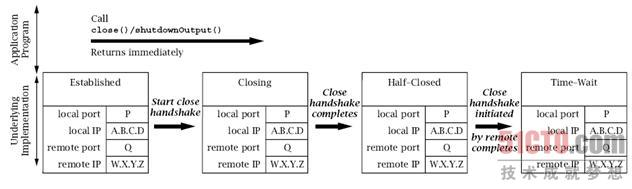
\includegraphics[scale=.6]{img/06.10.jpg}
			\caption{首先关闭一端的TCP连接}
			\label{fig:close.one.side.tcp}
		\end{figure}

		Application Program:应用程序;Underlying Implementation:底层实现;Call close()/shutdownOutput():调用close()/shutdownOutput()方法;Returns immediately:立即返回;Start close handshake:开始关闭握手;Close handshake completes:关闭握手完成;Close handshake initiated by remote completes:由远端发起的关闭握手完成;local port:本地端口;local IP:本地IP地址;remote port:远程端口号;remote IP:远程IP地址;

		在图6.10的右端时,netstat的输出内容包括:

		\lstinputlisting[language=Java,firstline=81,lastline=83]{src/ch06/stp.txt}

		图6.11简单展示了没有首先发起关闭的终端上的事件序列。关闭握手消息到达后,它立即发回一个确认消息,并将连接状态改变为"Close-Wait"。该主机上netstat的输出内容显示:

		\lstinputlisting[language=Java,firstline=85,lastline=87]{src/ch06/stp.txt}

		此时,只需要等待应用程序调用Socket的close()方法。调用该方法后,将发起最终的关闭握手消息,并释放底层套接字数据结构,虽然对原始Socket实例的引用仍然留存在Java程序中。

		注意这样一个事实:close()方法和shutdownOutput()方法都没有等待关闭握手的完成,而是调用后立即返回。你可能会问,发送者怎样能保证已发送的数据能够真正到底接收程序呢(即Delivered)?实际上,当应用程序调用close()或shutdownOutput()方法并成功关闭连接时,的确可能还有数据留存在SendQ队列中。如果连接的任何一端在数据传输到RecvQ队列之前崩溃,数据将丢失,而发送端应用程序却不会知道。

		最好的解决方案是设计一种应用程序协议,以使首先调用close()方法的一方在接收到了应用程序层的数据已接收保证后,才真正执行关闭操作。例如,当我们的TCPEchoClient程序接收到了它所发送的数据的完全拷贝后,它就能够知道此时在连接两个方向上都没有数据在传输,因此可以安全地关闭连接。


		\clearpage

		\begin{figure}[htbp]%位置选项
			\centering
			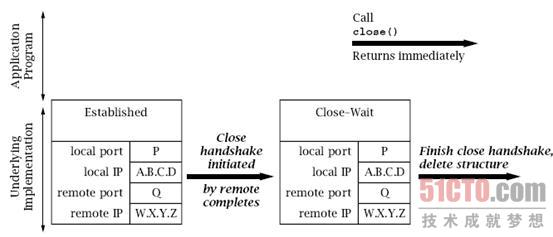
\includegraphics[scale=.6]{img/06.11.jpg}
			\caption{在另一端关闭后关闭TCP连接}
			\label{fig:close.other.side.side.tcp}
		\end{figure}

		Application Program:应用程序;Underlying Implementation:底层实现;Call close():调用close()方法;Return immediately:立即返回;Close handshake initiated by remote completes:远端发起的关闭握手完成;Finish close handshake, delete structure:完成关闭握手,删除数据结构;local port:本地端口;local IP:本地IP地址;remote port:远程端口号;remote IP:远程IP地址;

		Java的确提供了一种能够修改Socket的close()的行为的方法,即setSoLinger()方法。setSoLinger()用于控制close()方法在返回前是否等待关闭握手的完成。它有两个参数:一个布尔变量用来指示是否等待;一个整型变量用来指定放弃之前等待的时间(单位为秒)。也就是说,使用setSoLinger()设置了超时时间后,close()方法将阻塞等待,直到关闭握手完成或指定时间超时。然而,在本书的写作期间,即使在setSoLinger()设置的时间限制已经超过时,close()方法也没有提供任何信息来指示关闭握手的失败。换句话说,setSoLinger()方法没有为当前实现的应用程序提供任何额外担保。

		关闭TCP连接的最后微妙之处在于对Time-Wait状态的需要。TCP规范要求在终止连接时,两端的关闭握手都完成后,至少要有一个套接字在Time-Wait状态保持一段时间。这个要求的提出是由于消息在网络中传输时可能延迟。如果在连接两端都完成了关闭握手后,它们都移除了其底层数据结构,而此时在同样一对套接字地址之间又立即建立了新的连接,那么前一个连接在网络上传输时延迟的消息就可能在新连接建立后到达。由于其包含了相同的源地址和目的地址,旧消息就会被错误地认为是属于新连接的,其包含的数据就可能被错误地分配到应用程序中。

		虽然这种情形可能很少发生,TCP还是使用了包括Time-Wait状态在内的多种机制对其进行防范。Time-Wait状态用于保证每个TCP连接都在一段平静时间内结束,这期间不会有数据发送。平静时间的长度应该等于分组报文在网络上存留的最长时间的两倍。因此,当一个连接完全结束(即套接字数据结构离开Time-Wait状态并被删除),并为同样一对地址上的新连接清理道路后,就不会再有旧实例发送的消息还存留在网络中。实际上,平静时间的长度要依赖于具体实现,因为没有机制能真正限制分组报文在网络上能够延迟的时间。通常使用的时间范围是4分钟减到30秒,或更短。

		Time-Wait状态最重要的作用是,只要底层套接字数据结构还存在,就不允许在相同的本地端口上关联其他套接字。尤其是试图使用该端口创建新的Socket实例时,将抛出IOException异常。

\section{解调多路复用揭秘}

	在前面的讨论中已经隐含表明一个事实,即同一个机器上的不同套接字可以有相同的本地地址和端口号。例如,在只有一个IP地址的机器上,每个通过ServerSocket的accept()方法接收的新Socket实例都将使用与ServerSocket相同的本地端口号。显然,要确定传入的分组报文应该分配到那个套接字(即,解调多路复用)不仅仅是查看分组报文的目的地址和端口。


		\clearpage

	\begin{figure}[htbp]%位置选项
		\centering
		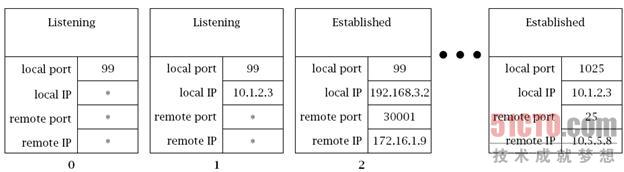
\includegraphics[scale=.6]{img/06.12.jpg}
		\caption{匹配了多个套接字的解调多路复用}
		\label{fig:match.muti.socket.ru}
	\end{figure}

	local port:本地端口;local IP:本地IP地址;remote port:远程端口号;remote IP:远程IP地址;

	否则传入的分组报文应该分配给哪个套接字就会含糊不清。对于TCP和UDP来说,将传入的分组报文匹配到某个套接字的过程是一样的,可以归纳为以下几点:

	套接字数据结构中的本地端口号必须与传入的分组报文的目的端口号相匹配。

	在套接字数据结构中,任何包含了通配符(*)的字段可以匹配分组报文中相应字段的任何值。

	如果有一个以上的套接字数据结构与传入的分组报文地址的四个字段匹配,那么谁使用的通配符少,谁就获得该分组报文。

	例如,考虑一个主机有两个IP地址的情况,10.1.2.3和192.168.3.2,还有如图6.12所示的活跃的TCP套接字数据结构子集。标记为0的数据结构与一个ServerSocket关联,有一个通配符本地地址,端口号为99。标记为1的套接字数据结构也关联了同一个端口号的ServerSocket,但其本地地址指定为10.1.2.3(因此它只接收发向这个地址的连接请求)。数据结构2代表了通过ServerSocket为数据结构0接收的一个连接,因此有相同的本地端口号,但也填入了本地和远程互联网地址。其他套接字则属于其他活跃的连接。现在考虑一个分组报文,其源IP地址是172.16.1.10,源端口号是56789,目的IP地址是10.1.2.3,目的端口号是99。该报文将分配到与数据结构1相关联的套接字上,因为该套接字匹配的通配符最少。

	当程序试图使用特定的本地端口号创建套接字时,要检查已有的套接字以确保没有其他套接字已经使用了那个本地端口。如果已经有套接字与构造函数中指定的本地端口和本地IP地址(如果有的话)相匹配,Socket的构造函数将抛出一个异常。这在如下情形中将导致一些问题:

	1.客户端程序用特定的本地端口号P创建了一个Socket实例,并通过它与服务器进行通信。

	2.客户端关闭了Socket,底层数据结构进入了Time-Wait状态。

	3.客户端程序终止后又立即重新启动。

	如果新的客户端化身试图使用同样的本地端口号,而由于其他数据结构正处于Time-Wait状态,Socket构造函数将抛出IOException异常。在写本书期间,解决这个问题的唯一途径是等待底层数据结构离开Time-Wait状态。

	那么怎么确定本地或远程的地址和端口号呢?对于ServerSocket,所有构造函数都要求传入本地端口号。本地地址可能会在构造函数中指定,否则,就使用通配符(*)地址。ServerSocket的远程地址和端口号始终是通配符。对于Socket,所有构造函数都要求传入特定的远程地址和端口号。本地地址或端口号可能会在构造函数中指定,否则,本地地址就使用用来建立到服务器的连接的网络接口地址,本地端口号就随机选择一个大于1023的未使用端口号。对于accept()方法返回的Socket实例,本地地址是从客户端发起的初始握手消息的目的地址,本地端口号是SeverSocket的本地端口,远程地址和端口号则是客户端的本地地址和端口号。对于DatagramSocket,本地地址和端口可能会在构造函数中指定,否则,本地地址将使用通配符地址,本地端口则随机选择一个大于1023的未使用端口号,远程地址和端口号都初始化为通配符并一直保持下去,除非调用connect()方法指定了特定的值。



	\part{其他扩展}

\end{document}
